\documentclass[DIV=14,headsepline,footsepline]{scrbook}
% header_phys.tex
% ----------------------------------------------------
% Lädt alle Header-Dateien für physikalische Dokumente
% ====================================================
%
% (Reihenfolge nicht ändern -> Führt sonst zu Fehlern)
%
% package.tex
% --------------------------------------------
% Headerdatei, die alle nötigen Packages lädt.
% ============================================
%
%
%  		Festlegen der Zeichencodierung des Dokuments und des Zeichensatzes.
%     Wir verwenden 'uft8' für das Dokument, da wir seit TxC standardmäßig UTF8-Dokumente erzeugen. Als Legacy-Option kann auch 'Latin1' 
%			(ISO-8859-1) für das Dokument gesetzt werden, wenn die Dateien in ANSI-Codierunge gespeichert werden.
%     Außerdem 'T1' Codierung für die Schrift.
%
\usepackage[utf8]{inputenc}
\usepackage[T1]{fontenc}
%
%  		Paket für die Lokalisierung ins Deutsche laden.
%     Wir verwenden neue deutsche Rechtschreibung mit 'ngerman'.
%
\usepackage[ngerman]{babel}
%
% 		Paket für Farben an verschieden Stellen. 
%     Wir definieren zusätzliche benannte Farben im 'style-header'.
%
\usepackage{color}
%
%			Paket für das Layout der Literaturangabe und 'Deutsche' Literaturangaben.
%
\usepackage[sort&compress, numbers]{natbib}
%
%			Paket für die \subfloat[]{}-Umgebung.
%
\usepackage[margin=1em, indention=1em]{subfig}
%
% 		Das Hyperref-Package verwenden. Spezielle Optionen werden gesondert erläutert.
%
\usepackage[
	pdfauthor={cand. phys. Erik Hänel},%				     											Autor des PDF Dokuments.
	pdfcreator={MiKTeX, LaTeX with hyperref and KOMA-Script},% 								Erzeuger/Kompiler des PDF Dokuments.
	bookmarksopenlevel={sections},%															 								PDF-Lesezeichen bis zu Sections öffnen.
	pdfpagemode={UseOutlines},%                                  								PDF-Lesezeichen beim Öffnen anzeigen.
	pdfdisplaydoctitle={true},%                                  								Dokumenttitel statt Dateiname in der Titelzeile anzeigen.
	pdfstartview={FitH}%																			 								Größe an Fensterbreite anpassen
]{hyperref}
%
%			Das Caption-Paket erlaubt, die Bildunterschriften der \subfloat[]{}-Umgebung zu formatieren.
%
\usepackage{caption}
\usepackage{array}		
\usepackage{graphicx}
\usepackage{tikz}
\usetikzlibrary{snakes}
\usepackage{epsfig}
%
%			AMS-MATH-Package mit der Option, die Grenzen bei Summen, Integralen und anderen Operatoren immer über und unter dem Symbol anzuzeigen.
%
\usepackage[sumlimits,intlimits,namelimits]{amsmath}
%
%			AMS-Packages für spezielle Symbole und Kommutative Diagramme
%
\usepackage{amssymb,amscd}
%
%			Symbole für Körper und Mengen (C,R,N,Q,etc.)
%
\usepackage{dsfont}
%
%			Schriftartensetup: Palatino für Textsatz und Pazomath für Mathesatz
%
\usepackage{mathpazo}
%
%			Schriftartensetup: Helvetica als serifenlose Schriftart und Courier für \texttt{}
%
\usepackage[scaled = 0.95]{helvet}
\usepackage{courier}
%
%			Spezialpackage: Erlaubt es, sich eigene Mathe-Akzente zu definieren. Findet hier bei dem Befehl \vhat{} Anwendung, der ein Hütchen mit 
%			einem Pfeil kombiniert.
%
\usepackage{accents}
%
%			Erweitert die Darstellung von Tabellen mit den Befehlen \toprule, \midrule & \bottomrule
%
\usepackage{booktabs}
%
%			Ermöglicht das direkte Tippen von Kommas ',' als Dezimaltrennzeichen. Erkennt dann aber keine Aufzählungen à la 1, 2, 3, ... mehr.
%
\usepackage{ziffer}
%
%			Dieses Package wird für den Befehl \mum verwendet, der 'µm' als Einheit definiert.
%
\usepackage{textcomp}
\usepackage{epstopdf}
%
% ========================================================
% EOF
%
% style_phys.tex
% -------------------------------------------------------------------
% Headerdatei, die das Aussehen und das Layout der Dokumente steuert.
% ===================================================================

%
%  1. Definieren von eigenen benannten Farben.
%     Für spätere Verwendung in dem Dokument, definieren wir einzelne
%     benannte Farben. Sie finden bei den Links, den Überschriften und die spezielle
%			'shadecolor' bei den farbigen Boxen (mit '\begin{shaded}\end{shaded}' gesetzt) Verwendung.
%
\definecolor{LinkColor}{rgb}{0,0,0.6}
\definecolor{HeadColor}{rgb}{0,0,0.5}
\definecolor{shadecolor}{rgb}{0.85,0.95,1}

%
%  2. KOMA-Script Option, Zeilenumbruch bei Bildbeschreibungen.
%
\setcapindent{1em}

%
%  3. Stil der Kopf- und Fusszeilen.
%     Wir aktivieren mit 'headings' laufende Seiten- /Kolumnentitel.
%
\pagestyle{headings}

%
%  4. Definieren der Schriftarten/Schiftfamilien der einzelnen Bereiche.
%
\setkomafont{chapter}{\huge\scshape\color{HeadColor}}       				% Kapitel farbig, Groß und als Kapitälchen
\setkomafont{section}{\Large\color{HeadColor}}											% Sections farbig und größer als normal
\setkomafont{captionlabel}{\sffamily\bfseries\color{HeadColor}}     % Fette Beschriftungstitel, farbig und serifenlos 
\setkomafont{caption}{\sffamily}																		% serifenlose Beschriftungen (tables/figures)
\setkomafont{pagehead}{\sffamily\bfseries\color{HeadColor}}         % Kolumnentitel serifenlos, farbig und fett
\setkomafont{descriptionlabel}{\sffamily\bfseries} 									% Fette und serifenlose Beschreibungstitel
\setkomafont{pagenumber}{\sffamily\bfseries}												% Fette, serifenlose Seitenzahlen
\setkomafont{part}{\Huge\scshape\color{HeadColor}}									% 'Part'-Titel Riesig, Kapitälchen und farbig

% Layouteinstellungen für "Subfloats": \subfloat[Titel]{\includegraphics[width=0.5\textwidth]{Pfad/zur/bilddatei.endung}}
\captionsetup[subfigure]{font={sf,footnotesize}, labelformat=simple, labelsep=colon}

%
%  5. Farbeinstellungen für die Links im PDF Dokument.
%
\hypersetup{%
	colorlinks=true,%        Aktivieren von farbigen Links im Dokument (keine Rahmen)
	linkcolor=LinkColor,%    Farbe festlegen.
	citecolor=LinkColor,%    Farbe festlegen.
	filecolor=linkColor,%    Farbe festlegen.
	menucolor=LinkColor,%    Farbe festlegen.
	urlcolor=LinkColor,%     Farbe von URL's im Dokument.
	bookmarksnumbered=true%  Überschriftsnummerierung im PDF Inhalt anzeigen.
}

%%%%%%%%%%%%%%%%%%%%%%%%%%%%%%%%%%%%%%%%%%%%%%%%%%%%%%%%%%%%
%
%  6. Die Besondere Formatierung der Kapitelüberschriften (Linien drüber und drunter)
%
 
% 1st get a new command
\newcommand*{\ORIGchapterheadstartvskip}{}%
% 2nd save the original definition to the new command
\let\ORIGchapterheadstartvskip=\chapterheadstartvskip
% 3rd redefine the command using the saved original command
\renewcommand*{\chapterheadstartvskip}{%
  \ORIGchapterheadstartvskip
  {%
    \setlength{\parskip}{0pt}%
    \noindent\rule[.3\baselineskip]{\linewidth}{1pt}\par
  }%
}
 
% see above
\newcommand*{\ORIGchapterheadendvskip}{}%
\let\ORIGchapterheadendvskip=\chapterheadendvskip
\renewcommand*{\chapterheadendvskip}{%
  {%
    \setlength{\parskip}{0pt}%
    \noindent\rule[.3\baselineskip]{\linewidth}{1pt}\par
  }%
  \ORIGchapterheadendvskip
}
%
%  End of chapter head change
%
%%%%%%%%%%%%%%%%%%%%%%%%%%%%%%%%%%%%%%%%%%%%%%%%%%%%%%%%%%%%
%
% ===========================================================================
% EOF
%
%	command.tex
% -------------------------------------------
%	Headerdatei, die alle nötigen Befehle lädt.
% ===========================================
%
% QM-spezifische Befehle: \bra{} (\tbra{}), \ket{} (\tket{}), \skal{}{} (\tskal{}{}) [Skalarprodukt], \EW{}, \ew{} [Erwartungswert]
%
\newcommand{\bra}[1]{\left\langle #1 \right|}
\newcommand{\tbra}[1]{\langle #1|}
\newcommand{\ket}[1]{\left| #1\right\rangle}					
\newcommand{\tket}[1]{| #1 \rangle}										
\newcommand{\skal}[2]{\left\langle #1 | #2 \right\rangle}
\newcommand{\tskal}[2]{\langle #1|#2\rangle}					
\newcommand{\EW}[1]{\left\langle #1 \right\rangle}		
\newcommand{\ew}[1]{\langle #1\rangle}
\newcommand{\vhat}[1]{\accentset{\hspace{1.6pt}\text{\fontsize{4.5pt}{4pt}{$\boldsymbol\wedge$}}\hspace{-3.9pt}\text{\fontsize{5pt}{4pt}{$\boldsymbol{\rightarrow}$}}}{#1}\hspace{0.4pt}}
%
% Allg. mathematische Befehle: \msakl [Skalarprodukt: <*,*>], \dx, \e, \eps, \prt{}{}, \Diff{}, \diff{}{}, \svec{}, \abs{}, \norm{}, \rot, 
%	\laplace
%
\newcommand{\mskal}[2]{\left\langle #1 , #2 \right\rangle}
\newcommand{\dx}{\:\mathrm{\normalfont{d}}}
\newcommand{\e}[1]{\:\mathrm{\normalfont{e}}^{#1}}
\newcommand{\eps}{\varepsilon}
\newcommand{\prt}[2]{\frac{\partial #1}{\partial #2}}
\newcommand{\diff}[2]{\frac{\mathrm{d} #1}{\mathrm{d} #2}} 
\newcommand{\Diff}[1]{\diff{}{#1}}									
\newcommand{\svec}[1]{\begin{pmatrix} #1 \end{pmatrix}} 
\newcommand{\detm}[1]{\begin{vmatrix} #1 \end{vmatrix}}
\newcommand{\abs}[1]{\left|#1\right|}									
\newcommand{\norm}[1]{\left\|#1\right\|}
\DeclareMathOperator{\rot}{rot}
\DeclareMathOperator{\divergence}{div}
\DeclareMathOperator{\erfc}{erfc}
\DeclareMathOperator{\erf}{erf}
\newcommand{\laplace}{{}\hspace{-0.3em}\mathrel{\rotatebox[origin=c]{180}{$\nabla$}}\hspace{-0.3em}}
%
% Abkürzungen für Mathematische Körper und Mengen
%
\newcommand{\N}{\mathds N}
\newcommand{\Z}{\mathds Z}
\newcommand{\R}{\mathds R}
\newcommand{\Q}{\mathds Q}
\newcommand{\C}{\mathds C}
\newcommand{\K}{\mathds K}
\newcommand{\V}{\mathds V}
\newcommand{\I}{\Im}
%
% Definition für µm
%
\newcommand{\mum}{\textmu m}
%
% Für Isotopenschreibweise von Elementen/Nukliden z.B. \chem{12}{6}C (Im gewöhnlichen Text)
% 
\newcommand{\chem}[2]{\shortstack[r]{\tiny{${#1}$}\\\scriptsize{$_{#2}$}}}
\newcommand{\sufo}[1]{\ensuremath{\mathrm{#1}}}
%
% Aufrecht gesetzter Indextext
%
\newcommand{\tx}[1]{_{\mathrm{#1}}}
%
% Der \vldt{} Befehl: Zeichet eine Linie, die das Argument als eine Marginalie auf dem Rand und über dem Strich darstellt. Spezialbefehl zum 
%	Datums-Ordnen von Vorlesungskripten
%
\newcommand{\vldt}[1]{\rule{0mm}{8mm}\textsf{\small{\textcolor{HeadColor}{$\blacktriangledown$ \textbf{Vorlesung vom #1}}}}
\marginline{\fbox{\textsf{\textbf{\small{\textcolor{HeadColor}{#1}}}}}}\newline\rule[.75\baselineskip]{\linewidth}{0.5pt}}
%
% Der \helpidx{} Befehl: Zeichet eine Linie, die das Argument als eine Marginalie auf dem Rand und über dem Strich darstellt. Spezialbefehl zum 
%	Datums-Ordnen von Vorlesungskripten
%
\newcommand{\helpidx}[1]{\noindent\rule{0mm}{5mm}\textsf{{\footnotesize\textcolor{HeadColor}{$\blacktriangleright$ \textbf{In the \textsc{NumeRe} documentation at:}}}} {\footnotesize\texttt{help #1}}
\marginline{\fbox{\texttt{\scriptsize{\textcolor{HeadColor}{#1}}}}}\newline\rule[.75\baselineskip]{\linewidth}{0.5pt}}
%
% Der \cmd{} Befehl: Zeichet eine Linie, die das Argument als eine Marginalie auf dem Rand und über dem Strich darstellt. Spezialbefehl zum 
%	Datums-Ordnen von Vorlesungskripten
%
\newcommand{\cmd}[1]{\marginline{\scriptsize\textsf{Syntax element}\\\texttt{\textbf{\scriptsize{\textcolor{red}{#1}}}}}}
%
%  Abkürzung für den \displaybreak[1]. Mit diesem Befehl kann man 'align'-Umgebungen beim Seitenende gezielt umbrechen.
%
\newcommand{\br}{\displaybreak[1]}
%
% Eine Erweiterung des \ref{label}-Befehls: Generiert einen Link, der Aus Objekttyp, Objektidentifikator und Objektcaption zusammengesetzt ist. 
% Bietet sich für Bezüge auf Abschnitte an: \fullref{sec:abschnitt} produziert z.B. 'Abschnitt 1.1 Abschnittstitel'
%
\newcommand{\fullref}[1]{\autoref{#1}: \nameref{#1}}
%
% Umgebung für eine alphabetisch nummerierte Liste
%
\newcounter{ale}
\newcommand{\abc}{\item[\alph{ale})]\stepcounter{ale}}
\newenvironment{liste}{\begin{itemize}}{\end{itemize}}
\newcommand{\aliste}{\begin{liste} \setcounter{ale}{1}}
\newcommand{\zliste}{\end{liste}}
\newenvironment{abcliste}{\aliste}{\zliste}
%	Setzen mit '\aliste\abc Text \zliste'
%
% ============================================
% EOF
%


% ====================================================
% EOF
%
\usepackage{xcolor}

\hypersetup{
	pdftitle={NumeRe Dokumentation},
	pdfsubject={NumeRe Dokumentation}
	}

\usepackage{listings}

\lstdefinelanguage{nscr}
{
	keywordsprefix=$,
	alsoletter={~\#},
	keywords=[2]{help,plot,mesh,copy,set,list,find,quit,load,show,stats,hist,fit,fitw,plot3d,dens,vect,vect3d,surf,new,remove,rename,delete,smooth,resample,edit,random,start,define,redefine,ifndefined,undefine,if,elseif,else,endif,while,endwhile,for,endfor,continue,break,matop,zeroes,extrema,integrate,diff,taylor,eval,datagrid,fft,odesolve,procedure,endprocedure,explicit,private,inline,var,str,return,namespace,throw,compose,endcompose,subplot,install,endinstall,uninstall,save},
	keywords={sin,cos,sqrt,avg,cmp,cnt,max,med,min,norm,num,prd,std,sum,to_char,sinc,to_value,to_cmd,valtostr,to_string,string_cast,matfc,zero,exp},
	sensitive=true
	morecomment=[l]{\#\#},
	morecomment=[s]{\#*}{*\#},
	string=[b]"
}
\newcommand\realnumberstyle[1]{\tiny}
\makeatletter
\newcommand{\zebra}[3]{%
    {\realnumberstyle{#3}}%
    \begingroup
    \lst@basicstyle
    \ifodd\value{lstnumber}%
        \color{#1}%
    \else
        \color{#2}%
    \fi
        \rlap{\hspace*{\lst@numbersep}%
        \color@block{\linewidth}{\ht\strutbox}{\dp\strutbox}%
        }%
    \endgroup
}
\makeatother

\definecolor{CommandStyle}{RGB}{0,128,255}
\definecolor{StringStyle}{RGB}{128,128,255}
\definecolor{BGColorTwo}{RGB}{245,245,245}
\definecolor{BGColorOne}{RGB}{230,230,230}
\definecolor{CommentStyle}{RGB}{0,128,0}
\lstset{
	language=nscr,
	basicstyle={\small\ttfamily},
	extendedchars=true,
	tabsize=4,
	columns=fixed,
	keepspaces=false,
	breaklines=true,
	showstringspaces=false,
	numbers=left, numberstyle=\tiny, stepnumber=2, numbersep=5pt,
	commentstyle=\color{CommentStyle},
	ndkeywordstyle={\color{CommandStyle}\bfseries\underbar},
	keywordstyle={\color{blue}\bfseries},
	stringstyle=\color{StringStyle},
	backgroundcolor=\color{BGColorTwo},
}





\newcommand{\NR}{\textsc{Nu\-me\-Re}}

\begin{document}
	\subject{Dokumentation}
	\title{\textsc{\textcolor{HeadColor}{NumeRe: Framework für Numerische Rechnungen}}}
	\subtitle{1.0.x-Serie\\Freie numerische Software unter der GNU GPL v3}
	\author{Erik Hänel et al.}
	\publishers{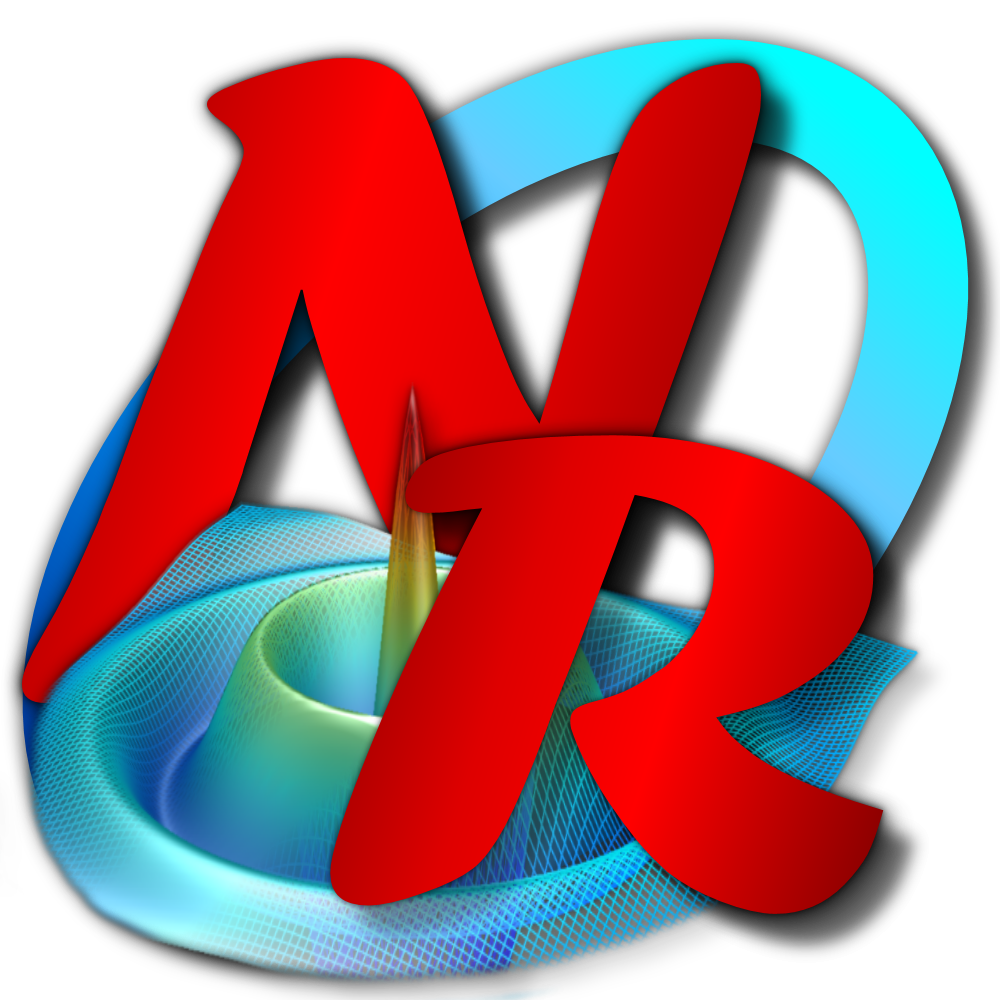
\includegraphics[width=0.5\textwidth]{_graphics/folder.png}}
	\dedication{\emph{Für die Freunde der Wissenschaft}}
	\maketitle
	\tableofcontents
	
	\addchap{Rechtliche Informationen}
		\addsec{GNU Free Documentation Licence v1.2}
			{\scriptsize--- Lizenz dieser Dokumentation ---}\smallskip\\
			\textbf{Copyright \copyright\ 2016, Erik Hänel.}
			
			Kopieren, Verbreiten und/oder Modifizieren ist unter den Bedingungen der GNU Free Documentation Licence, Version 1.2 oder einer späteren Version, veröffentlicht von der Free Software Foundation, erlaubt. Es gibt keine unveränderlichen Abschnitte, keinen vorderen Umschlagtext und keinen hinteren Umschlagtext. Eine Kopie des Lizenztextes ist unter \href{http://www.gnu.org/copyleft/fdl.html}{GNU Free Documentation Licence} zu finden.
		\addsec{GNU General Public Licence v3}
			{\scriptsize--- Lizenz des Programms und der gezeigten Codefragmente ---}\smallskip\\
			\textbf{Copyright \copyright\ 2016, Erik Hänel et al.}
			
			Das beschriebene Programm und die hier gezeigten Codefragmente sind freie Software. Sie können es unter den Bedingungen der GNU General Public License, wie von der Free Software Foundation veröffentlicht, weitergeben und/oder modifizieren, entweder gemäß Version 3 der Lizenz, oder (nach Ihrer Option) jeder späteren Version.
			
			Die Veröffentlichung dieses Programms erfolgt in der Hoffnung, dass es Ihnen von Nutzen sein wird, aber OHNE IRGENDEINE GARANTIE, sogar ohne die implizite Garantie der MARKTREIFE oder der VERWENDBARKEIT FÜR EINEN BESTIMMTEN ZWECK. Details stehen in der GNU General Public Licence.
			
			Sie sollten ein Exemplar der GNU GPL zusammen mit diesem Programm erhalten haben. Falls nicht, siehe \href{http://www.gnu.org/licenses/}{www.gnu.org/licenses/}.
		\addsec{Mitwirkende}
			\begin{itemize}
				\item \textbf{Konzept/UI:} Erik \textsc{Hänel}
				\item \textbf{Mathe-Parser:} Ingo \textsc{Berg}, Erik \textsc{Hänel} (muParser)
				\item \textbf{Plotting:} Alexey \textsc{Balakin} (MathGL)
				\item \textbf{numerische Algorithmen:} GNU Scientific Library
				\item \textbf{Tokenizer:} Boost-Library
				\item \textbf{Matrix-Algorithmen:} Eigen-Library
				\item \textbf{XML-Parser:} Lee \textsc{Thomason} (TinyXML-2)
				\item \textbf{Excel-(97-2003)-Funktionalität:} \textsc{Yap Chun} Wei (BasicExcel)
				\item \textbf{Testing:} D.~\textsc{Bammert}, J.~\textsc{Hänel}, R.~\textsc{Hutt}, K.~\textsc{Kilgus}, E.~\textsc{Kloster}, K.~\textsc{Kurz}, M.~\textsc{Löchner}, L.~\textsc{Sahinov\'c}, D.~\textsc{Schmid}, V.~\textsc{Sehra}, G.~\textsc{Stadelmann}, R.~\textsc{Wanner}, F.~\textsc{Wunder}, J.~\textsc{Zinßer}
			\end{itemize}
	\addchap{Installation}
		Seit Version v1.0.7 ">Bose"< wird \NR\ in Form eines Installers auf \href{https://sourceforge.net/projects/numere/files/latest/download}{SourceForge} veröffentlicht. Um \NR\ auf dem eigenen Rechner zu installieren, muss der Installer heruntergeladen und ausgeführt werden. Nachdem man den entsprechenden Schritten gefolgt ist, ist \NR\ auf dem eigenen Rechner installiert und kann ausgeführt werden.
		
		Um eine neuere Version von \NR\ zu installieren, muss (und sollte) die vorherige Version \emph{nicht} deinstalliert werden. Die neuere Version kann direkt über die bereits existierende installiert werden.
		\paragraph{Anmerkung}
			Der Installer gibt als Standardpfad ">C:/Software/NumeRe"< vor. Dieser Pfad kann geändert werden, jedoch sollte auf ">C:/Programme/\ldots"< bzw. ">C:/Programme (x86)/\ldots"< verzichtet werden. An diesen Orten kann \NR\ unter Umständen nicht korrekt ausgeführt werden.
		\addsec{Systemvoraussetzungen}
			\NR\ kann auf allen Desktop-Windowsversionen von XP bis 10 ausgeführt werden. Für Windows 8.1 und 10 muss die zusätzliche Komponenten-Kompatibilität installiert werden, da es anderenfalls zu Abstürzen während des Plotvorgangs kommen kann.
			
			Außerdem erfordert \NR\ eine Tastatur zur korrekten Ausführung. Die Bildschirmtastatur kann ggf. auch verwendet werden, ist aber weniger komfortabel.
		\addsec{Portable und Stable Version}
			Standardmäßig wird die Installation der Stable Version empfohlen, welche die Dateiverknüpfungen für \NR\ vornimmt. Dabei werden Administratorrechte vorausgesetzt. Die Portable Version kann auch ohne Administratorrechte ausgeführt werden, legt dabei aber keine Dateiverknüpfungen an. \NR-Portable kann aber (prinzipiell) von jedem Verzeichnis aus gestartet, beliebig verschoben und zum Deinstallieren einfach gelöscht werden.
			\paragraph{Anmerkung}
				Der ">Stable Version"<-Installer schreibt lediglich die Dateiverküpfungen und den Link zum Uninstaller in die Windows-Registry. Es werden keine Konfigurationen oder andere für die Programmausführung relevante Daten in die Registry geschrieben.
	\part{Grundlegende Bedienung}
		\chapter{Erste Schritte}
			Aller Anfang ist schwer. Das ist uns sehr wohl bewusst, daher haben wir hier die wesentlichen ersten Dinge zusammengetragen, die den Einstieg in \NR\ leichter gestalten sollen. Allerdings erhebt diese Dokumentation natürlich keinen Anspruch auf Vollständigkeit. Die Feinheiten aller Optionswerte werden hier ebenfalls nicht beschrieben. Eine Beschreibung derselben findet man in der integrierten Dokumentation.
			\paragraph{Anmerkung}
				Diese Dokumentation ist mit Marginalien ausgestattet, die auf Aktionen in \NR\ verweisen sollen. Marginalien in rot sind Syntaxelemente, die in die \NR-Konsole eingegeben werden können. Gerahmte Marginalien in dunkelblau bezeichnen Artikel der integrierten \NR-Hilfe.
			\section{Das User Interface}
				\textbf{Hilfe!}
				
				Das werden die meisten denken, sobald sie \NR\ zum ersten Mal starten werden, denn \NR\ besteht nahezu vollständig aus Textkommandos. Und die Benutzeroberfläche -- hier auch \emph{User Interface} genannt -- ist die standardmäßige Windowskonsole (\autoref{fig:ui_0}), die man auch mittels Start $\Rightarrow$ Ausführen $\Rightarrow$ ">cmd.exe"< erreichen kann. Hier ist nichts mit Klicken und Mausbedienung. Was jetzt erst mal wie ein Nachteil wirkt, wird sich im Laufe der Verwendung alsbald relativieren.
				
				Jetzt heißt es erst mal
				\begin{quotation}
					\noindent\emph{Tief durchatmen, den Schreck überwinden und das Programm genauer unter die Lupe nehmen.}
				\end{quotation}
				\begin{figure}[p]%
					\centering
					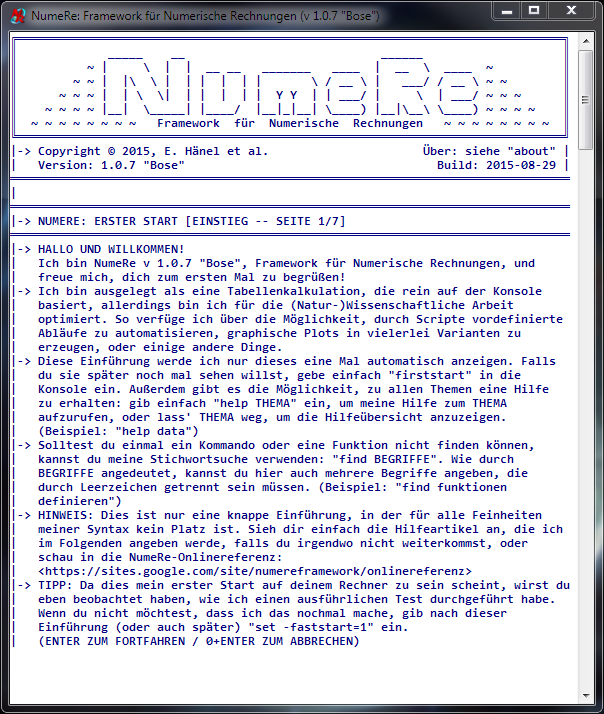
\includegraphics[width=0.9\textwidth]{_graphics/ui_0.png}
					\caption{\NR's erster Start zeigt eine Einführung. Die Schriftart lässt sich mittels Rechtsklick auf die Titelleiste des Fensters zu z.B. ">Consolas"< ändern}
					\label{fig:ui_0}
				\end{figure}
				
				\NR\ zeigt beim ersten Start automatisch eine kurze Einführung in das Programm an, die im Wesentlichen eine Zusammenfassung dieser Dokumentation ist (\autoref{fig:ui_0}). Die Feinheiten und Fähigkeiten von \NR\ können hierin aber allerhöchstens kurz angeschnitten werden. Die Einführung richtet sich daher eher an diejenigen, die schon einmal mit einem zu \NR\ ähnlichen Programm zu tun hatten.
				
				Um die nächsten Seiten aufzurufen, bestätigt man wiederholt mit [ENTER]. Um die Einführung hingegen abzubrechen, gibt man \verb+0+ ein und bestätigt mit [ENTER]. Um die Einführung später aufzurufen, kann \verb+firststart+ in die Konsole eingegeben werden.
				
				Nach der Einführung kann \NR\ wie in dieser Dokumentation aufgeführt bedient werden. Dabei erscheint am Anfang der Zeile ein Pfeil \verb+<-+, der verdeutlichen soll, dass hier eine Eingabe erwartet wird (\autoref{fig:ui_1}). Ausgaben, die das Programm tätigt, werden alle durch den entgegen gerichteten Pfeil \verb+->+ begonnen. Es können \emph{nur dann} Eingaben getätigt werden, wenn ein solcher Pfeil (oder die explizite Aufforderung) erscheint.
				
				\paragraph{Anmerkung}
					In einem späteren Kapitel werden Verzweigungen und Schleifen beschrieben. In diesen Fällen ändert sich der Pfeil am Anfang der Zeile zu einem spezielleren Symbol. Dies soll an dieser Stelle aber nicht weiter von Bedeutung sein.
				\bigskip\\
				In die \NR-Konsole können an dieser Stelle sowohl mathematisch-numerische Ausdrücke als auch Kommandos eingegeben werden. Die Syntax der mathematisch-numerischen Ausdrücke ist recht intuitiv und wird im übernächsten Abschnitt nochmals erläutert. Die Syntax der Kommandos bedarf hingegen einer kurzen Erläuterung.
				
				Es wurde versucht, \NR\ so intuitiv wie irgend möglich zu gestalten. Diese Prämisse war auch für die Kommandosyntax vorgegeben, ist aber aufgrund der Tatsache, dass \NR\ ein ">gewachsenes"< Programm ist, an ein paar Stellen vielleicht nicht wirklich erfüllt. Dennoch halten sich die Kommandos alle an dasselbe Schema:
				\begin{verbatim}
					KOMMANDO [AUSDRUCK] [-PARAMETER[=WERT] [OPTIONEN[=WERT]]]
				\end{verbatim}
				Syntaxelemente in eckigen Klammern sind teils optional teils nicht bei jedem Kommando vorhanden. Beispiele für die Kommandosyntax sind
				\begin{lstlisting}
help
help expression
plot sin(x)
mesh sin(x)+cos(y) -set box
copy <>/samples/data* -target=<loadpath>/*
				\end{lstlisting}
				Hier ist zu sehen, dass (manche) Kommandos nicht zwangsläufig einen Ausdruck oder einen Parameter benötigen.
				
				Die erst einmal gewöhnungsbedürftige Kommandosyntax wird durch den ">Merksatz"< 
				\begin{quotation}
					\noindent\emph{">Führe eine Aktion [auf etwas] aus und verwende dabei die folgenden Parameter."<}
				\end{quotation}
				vermutlich etwas eingängiger. Auf die obigen Beispiele ausgeführt, könnte dies zum Beispiel
				\begin{quotation}
					\noindent\emph{">Öffne die Hilfe, die sich mit ">expression"< befasst."<}
				\end{quotation}
				oder
				\begin{quotation}
					\noindent\emph{">Generiere einen Gitterplot der Funktion ">sin(x)+cos(y)"< und verwende eine umfassende Box."<}
				\end{quotation}
				lauten.
				\begin{figure}[p]%
					\centering
					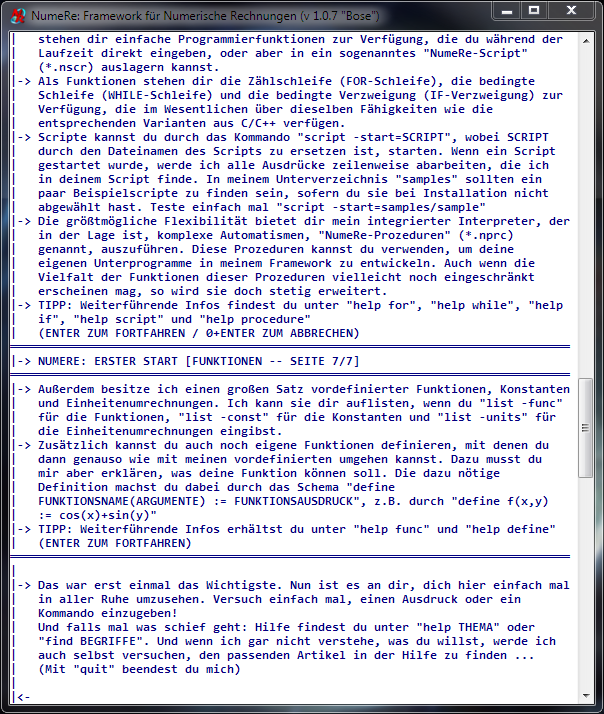
\includegraphics[width=0.9\textwidth]{_graphics/ui_1.png}
					\caption{Nach den 7 Seiten der Einführung kann \NR\ wie in dieser Dokumentation beschrieben bedient werden. Durch den Pfeil am Anfang der Zeile wird angedeutet, dass eine Eingabe erwartet wird}
					\label{fig:ui_1}
				\end{figure}
				
				\helpidx{syntax}
				\cmd{list}Verwendet man das Auflistungskommando mit dem Parameter \verb+cmd+
				\begin{lstlisting}
list -cmd
				\end{lstlisting}
				so wird eine Liste aller Kommandos zuzüglich einer schematischen Syntax angezeigt. Sollte auch dies nicht weiterhelfen, so kann der zum Kommando gehörende Artikel der \NR-Hilfe aufgerufen werden, z.B. durch\cmd{help}
				\begin{lstlisting}
help plot
				\end{lstlisting}
				In diesen Artikeln finden sich alle Parameter und Syntaxinformationen, sowie ein Beispiel der Syntax, die für die korrekte Ausführung nötig sind.
				
				\helpidx{numere}
				Sollte einmal eine Eingabe fehlerhaft sein, wird \NR\ eine entsprechende Meldung auf die Konsole ausgeben. Wenn eine mathematisch-numerischer Ausdruck fehlerhaft ist, wird die Position des Fehlers -- sofern zutreffend -- mit ausgegeben. Bei Fehlern in der Verwendung der Kommandosyntax gibt \NR\ neben der Meldung auch eine Referenz auf den entsprechenden Hilfeartikel zurück.
				
				Ausdrucks- und Kommandofehler werden sämtliche Auswertungen abbrechen. Demzufolge werden auch \NR-Scripte und \NR-Prozeduren mit Ausgabe der entsprechenden Meldung abgebrochen.
			\section{Einstellungen}
				Alle Einstellungen in \NR\ werden mit dem Kommando \verb+set+ durchgeführt. Als Parameter muss dabei die Bezeichnung der Einstellung und der gewünschte Wert folgen:\cmd{set}
				\begin{lstlisting}
set -EINSTELLUNG=WERT
				\end{lstlisting}
				Falls der Wert der Einstellung Leerzeichen enthält (z.B. in einem Dateipfad), muss dieser mit umschließenden Anführungszeichen angegeben werden:
				\begin{lstlisting}
set -EINSTELLUNG="WERT MIT LEERZEICHEN"
				\end{lstlisting}
				Das \verb+list+-Kommando kann eine Auflistung aller Einstellungen anzeigen:\cmd{list}
				\begin{lstlisting}
list -settings
				\end{lstlisting}
				Eigentlich sind alle Einstellungen, die \NR\ mitbringt, bereits sinnvoll.
				
				\helpidx{set}
				Die erste Einstellung, die man tätigen sollte, ist die Verknüpfung von \NR\ mit einem externen Bildbetrachter (in diesem Kontext auch \emph{viewer} genannt). Hierbei bietet sich vor allem \href{http://www.irfanview.net}{IrfanView} an. Falls man diesen installiert hat, kann man ihn mit \NR\ verknüpfen:
				\begin{lstlisting}
set -viewer="C:/Program Files/IrfanView/i_view32.exe"
				\end{lstlisting}
				Hierbei sei angemerkt, dass auf 64-Bit-Systemen der Dateipfad zu ">C:/Program Files (x86)/\ldots"< geändert werden muss. Als Texteditor ist der Windows-Editor vorgegeben. Aber auch dieser kann zum Beispiel zu \href{https://notepad-plus-plus.org/}{Notepad++} geändert werden:
				\begin{lstlisting}
set -editor="C:/Program Files/Notepad++/notepad++.exe"
				\end{lstlisting}
				
				Die Angabe eines eigenen Viewers und eines Editors kann die Arbeit mit \NR\ deutlich vereinfachen, da die erzeugten Graphen dann automatisch angezeigt werden und speziell für Notepad++ eine eigene Syntaxhervorhebung vorhanden ist.
				
				\helpidx{viewer}
				Die geänderten Einstellungen werden zum Programmende hin gespeichert und sind bei einem Neustart wieder verfügbar.
			\section{Einfache Rechnungen}
				\NR\ kann als Framework für numerische Rechnungen natürlich numerisch rechnen. Die zu berechnenden Gleichungen können ähnlich wie in einen Taschenrechner eingegeben werden. Abstände zwischen Operatoren und Werten spielen natürlich keine Rolle, allerdings dürfen zwischen Funktionsnamen und ihren Argumentklammern (ebenso bei den späteren Tabellenobjekten) \emph{keine} Leerzeichen sein. Daneben wird zwischen Groß- und Kleinschreibung unterschieden und der Malpunkt \verb+*+ muss stets mit eingegeben werden:
				\begin{lstlisting}
5*cos(_2pi)
				\end{lstlisting}
				multipliziert $\cos2\pi$ mit 5 und gibt das Ergebnis direkt aus (\autoref{fig:first_calc_0}). Als Dezimaltrennzeichen wird der Punkt \verb+.+ verwendet: die Zahl \verb+5.2+ ist in deutscher Dezimalschreibweise folglich identisch zu 5,2. \verb+_2pi+ ist dabei eine vordefinierte Konstante für $2\pi$ und \verb+cos()+ ist natürlich die Kosinus-Funktion.
				\begin{figure}[p]%
					\centering
					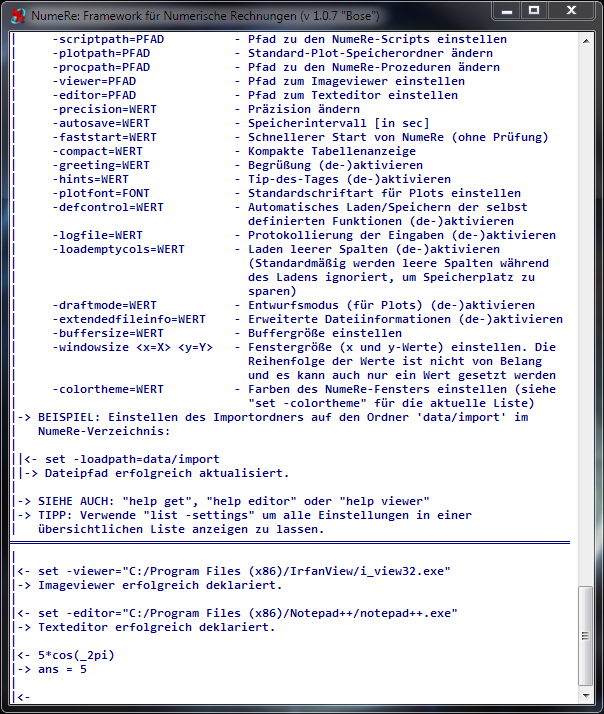
\includegraphics[width=0.9\textwidth]{_graphics/first_calc_0.png}
					\caption{\NR\ nach Eingabe der ersten Rechnung}
					\label{fig:first_calc_0}
				\end{figure}
				Die vordefinierten Konstanten und Funktionen können mittels 
				\begin{lstlisting}
list -const
list -func
				\end{lstlisting}
				aufgelistet werden. \verb+list -func+ kann noch weiter eingeschränkt werden.
				
				\helpidx{list}
				\NR\ kann aber nicht nur mit Zahlen umgehen, sondern auch mit Variablen. Die Variablen \verb+x+, \verb+y+, \verb+z+, \verb+t+ und \verb+ans+ sind bereits vordefiniert. Es können aber auch weitere Variablen definiert werden. Das geschieht entweder automatisch (sobald \NR\ auf eine unbekannte Variable stößt) oder durch eine direkte Zuweisung:
				\begin{lstlisting}
neue_variable = 5
				\end{lstlisting}
				Hier wird die neue Variable \verb+neue_variable+ mit dem Wert 5 definiert. Die obige Gleichung kann damit auch auf folgende Art geschrieben werden:
				\begin{lstlisting}
neue_variable*cos(_2pi)
				\end{lstlisting}
				
				\NR\ kann auch mehrere Ausdrücke zugleich auswerten. Die Ausdrücke müssen dabei durch jeweils ein Komma \verb+,+ getrennt sein. Innerhalb dieser Ausdrücke wird von links nach rechts vorgegangen. Die Zeile 
				\begin{lstlisting}
neue_variable = 5, neue_variable*cos(_2pi), neue_variable = 1
				\end{lstlisting}
				setzt \verb+neue_variable+ auf 5, berechnet $5\cos2\pi$ und setzt \verb+neue_variable+ anschließend auf 1 (\autoref{fig:first_calc_1}). In Schleifen kann diese Schreibweise erhebliche Geschwindigkeitsvorteile bringen.
				
				\helpidx{expression}
				\begin{figure}[p]%
					\centering
					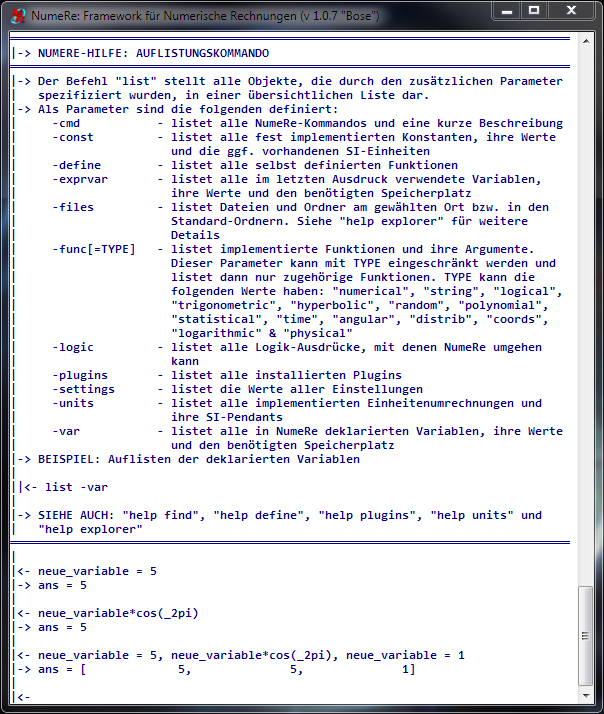
\includegraphics[width=0.9\textwidth]{_graphics/first_calc_1.png}
					\caption{\NR\ nach Eingabe der letzten Rechnung}
					\label{fig:first_calc_1}
				\end{figure}
			\section{Wichtige Kommandos}
				\NR\ wird nur durch Kommandos bedient. Die wichtigsten Kommandos sind hierbei\cmd{help\\find\\list\\quit}
					\begin{lstlisting}
help
help THEMA
find BEGRIFFE
list -OBJEKT
quit
					\end{lstlisting}
					Diese Kommandos rufen die integrierte Dokumentation (\verb+help+ bzw. \verb+help THEMA+ zum THEMA), die Stichwortsuche (\verb+find BEGRIFFE+) auf, listen OBJEKTE (\verb+list -OBJEKT+) und beenden \NR\ (\verb+quit+). Sie werden bei jedem Programmstart am Anfang nochmals angezeigt (\autoref{fig:ui}).
					\begin{figure}[p]%
						\centering
						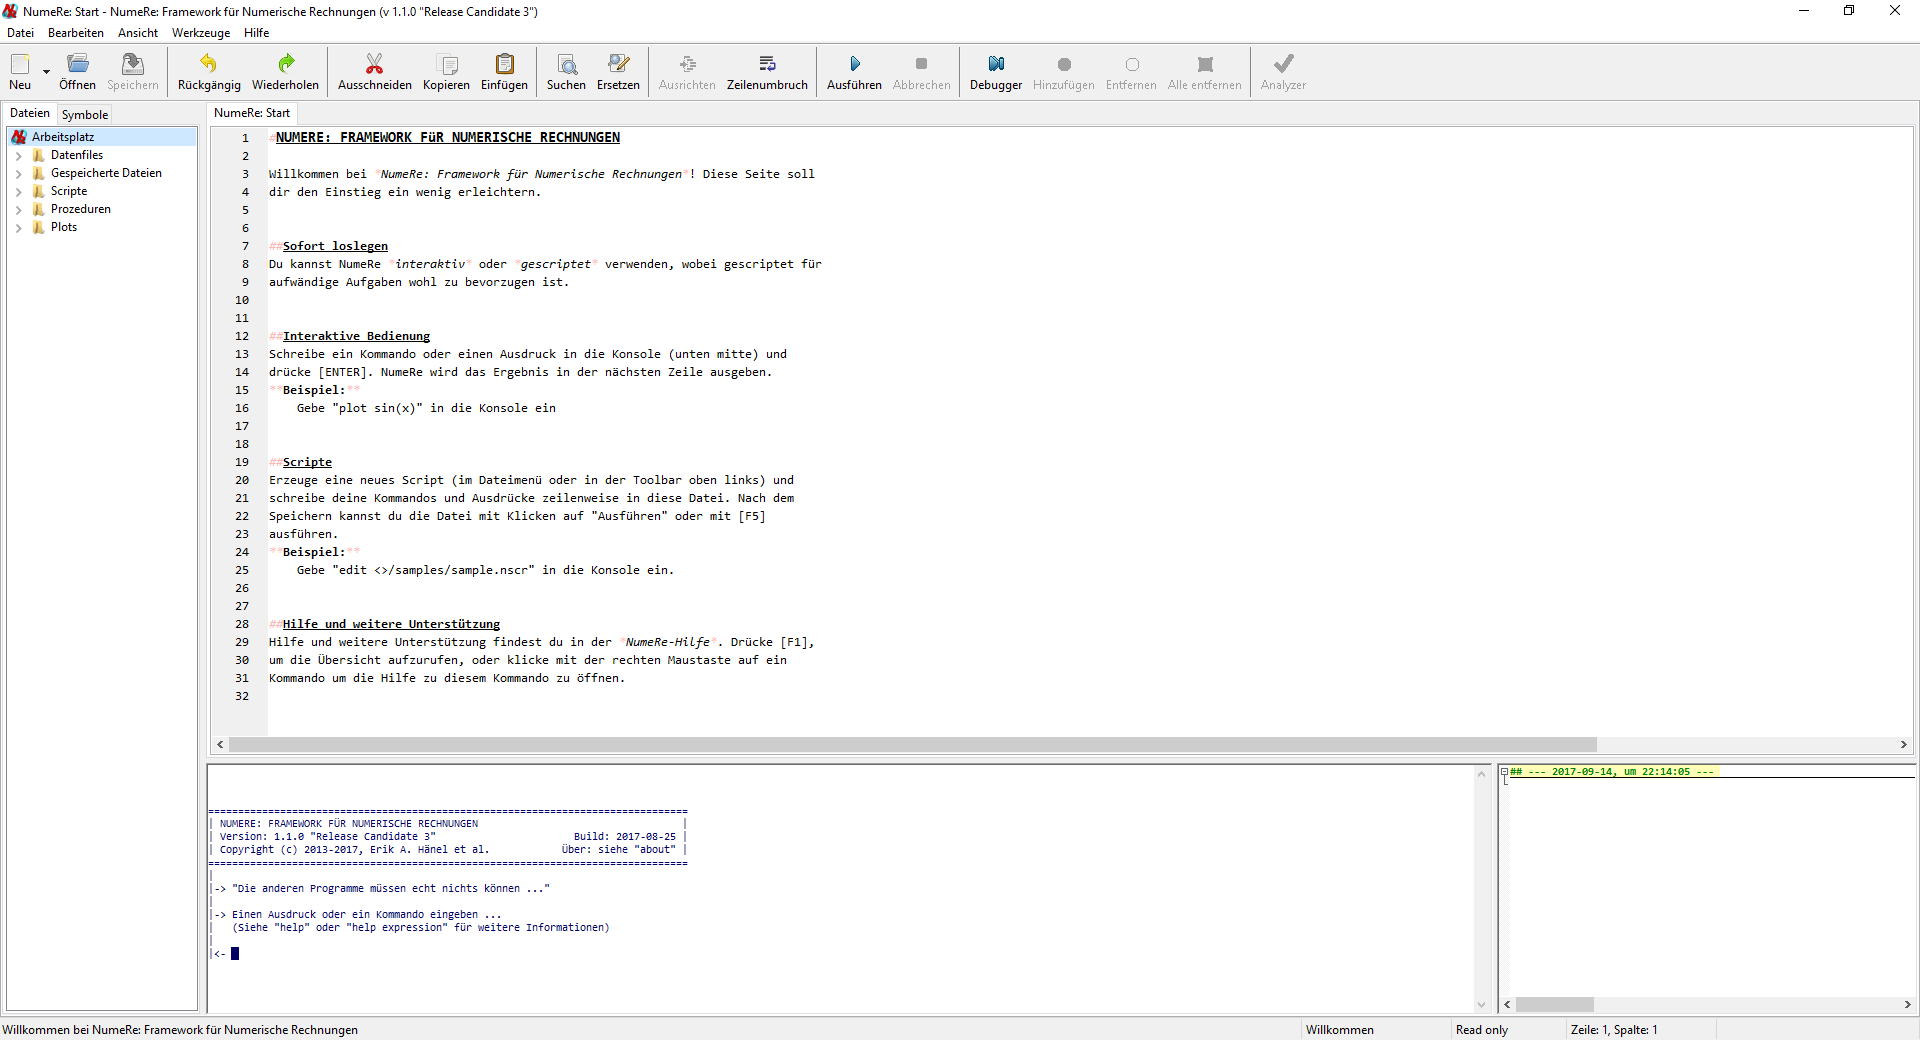
\includegraphics[width=0.9\textwidth]{_graphics/ui.png}
						\caption{Die Startansicht von \NR\ mit der Auflistung der wichtigsten Kommandos}
						\label{fig:ui}
					\end{figure}
					
					Eine komplette Liste aller Kommandos erhält man durch 
					\begin{lstlisting}
list -cmd
					\end{lstlisting}
					Diese Auflistung enthält auch eine knappe Beschreibung sowie eine symbolische Syntax der Kommandos.
					
					Alle Kommandos haben einen Eintrag in der \NR-Hilfe. Dieser Artikel kann durch die Eingabe von \verb+help KOMMANDO+ angezeigt werden und enthält alle Informationen zu einem Kommando und ggf. noch Referenzen auf weitere wichtige Dokumentationsartikel. Im Falle, dass eine Information einmal nicht direkt in der \NR-Hilfe gefunden werden kann, kann die Stichwortsuche (\verb+find+) große Dienste erweisen, da selbige auch direkt passende Artikel der \NR-Hilfe liefert.
					\paragraph{Anmerkung}
						Mittels Semikola ">\verb+;+"< können auch mehrere Kommandos und mehrere Ausdrücke, die nacheinander auszuwerten sind, gemeinsam in einer Zeile angegeben werden:
						\begin{lstlisting}
KOMMANDO1; KOMMANDO2; AUSDRUCK1; KOMMANDO3; AUSDRUCK2; ...
						\end{lstlisting}
		\chapter{Daten laden und verwenden}
			Da ein großer Teil der wissenschaftlichen Arbeit auf der Datenanalyse beruht, ist es notwendig, Programme zu verwenden, die entsprechende Datenmengen in einem vernünftige Zeitrahmen laden und verarbeiten können. \NR\ interpretiert alle gelesen Daten in einer tabellarischen Darstellung und kann Statistiken, Histogramme und fortgeschrittenere Auswertungen durchführen.
			\section{Dateitypen}
				Neben reinen Textdateien im ANSI-Format (Dateiendungen *.txt und *.dat) kann \NR\ die folgenden Dateiformaten lesen:
				\begin{itemize}
					\item \textbf{CassyLab-Datei (*.labx).} Dieser Datentyp wird nur von CassyLab verwendet und enthält ein komplettes CassyLab-Experiment. \NR\ wird jedoch nur die tabellarischen Daten extrahieren.
					\item \textbf{CSV-Datei (*.csv).} Comma-Separated-Values-Dateien sind ein Quasi-Standard zum Austauschen von Daten. Allerdings existiert kein ">CSV-Standard"<, so dass es trotz umfassenden Tests vorkommen kann, dass eine CSV-Datei nicht korrekt interpretiert werden kann. (Der Programmierer freut sich über eine entsprechende Bugmeldung inkl. der angehängten Datei.)
					\item \textbf{JCAMP-DX-Datei (*.dx, *.jdx und *.jcm).} JCAMP-DX-Dateien (von \emph{Joint Committee on Atomic and Molecular Physical data -- Data eXchange}) sind ein Dateistandard für den Austausch von Spek\-tro\-sko\-pie-Daten. \NR\ wird auch aus diesen Dateien nur die tabellarischen Daten extrahieren.
					\item \textbf{OpenDocument-Spreadsheet (*.ods).} Tabellarische Daten, die z.B. von OpenOffice Calc erzeugt wurden. \NR\ wird hier nur die numerischen Werte und die Zeichenketten, jedoch nicht die Gleichungen lesen. Zu beachten ist, dass OpenOffice Calc geöffnete Dateien \emph{lockt}: Spreadsheets, die in OpenOffice Calc geöffnet sind, können \emph{nicht} von \NR\ gelesen werden.
					\item \textbf{Excel-Workbooks (*.xls und *.xlsx).} Tabellarische Daten, die z.B. von Excel erzeugt wurden. \NR\ wird hier nur die numerischen Werte und die Zeichenketten, jedoch nicht die Gleichungen lesen. Eine Einschränkung des alten Excelformates ist zusätzlich, dass Ergebnisse, die durch Gleichungen berechnet wurden, ebenfalls nicht gelesen werden können. Zu beachten ist außerdem, dass Excel wie OpenOffice Calc geöffnete Dateien \emph{lockt}: Workbooks, die in Excel geöffnet sind, können \emph{nicht} von \NR\ gelesen werden.
					\item \textbf{IGOR Binary Waves (*.ibw).} IGOR Binary Waves enthalten die Daten einer (1-, 2- oder 3-dimensionalen) IGOR-Welle.
					\item \textbf{NumeRe-Datenfile (*.ndat).} NumeRe-Datenfiles sind ein \NR-eigenes, binäres Dateiformat zum schnellen Speichern und Lesen der Datensätze.
				\end{itemize}
				
				\helpidx{load}
				\NR\ kann jedoch nicht alle Formate schreiben. Als Ausgabeformate stehen die folgenden zur Verfügung:
				\begin{itemize}
					\item \textbf{Textdatei (*.dat oder *.txt).} \NR\ erzeugt eine Textdatei in ANSI-Codierung, die dem Formatierungsstandard des folgenden Abschnitts genügt. Diese Textdateien sollten von den meisten anderen Programmen gelesen werden können
					\item \textbf{NumeRe-Datenfile (*.ndat).} Dieses Dateiformat kann (nur) von \NR\ gelesen werden. Das Dateiformat ist jedoch online dokumentiert und kann in andere Programme implementiert werden.
					\item \textbf{CSV-Datei (*.csv).} \NR\ erstellt eine CSV-Datei mit Kommata \verb+,+ als Spalten- und Punkten \verb+.+ als Dezimaltrennzeichen. (Möglicherweise kann dies von gewöhnlichen Tabellenkalkulationen nicht korrekt gelesen werden: das Ersetzen der Kommata durch Semikola \verb+;+ und der Punkte durch Kommata behebt dieses Problem gegebenenfalls. Der Grund hierfür entzieht sich dem Programmierer.)
					\item \textbf{Excel Workbook (*.xls).} \NR\ kann die Daten im alten Excel-(97-2003)-Format (*.xls) exportieren, so dass sie in Excel und Konsorten weiterverarbeitet werden können.
					\item \textbf{\TeX-Datei (*.tex).} \NR\ schreibt eine Tabelle im \TeX-Format. In den Kommentaren der erzeugten Datei finden sich die Voraussetzungen, um die erzeugte Tabelle in ein \TeX-Do\-ku\-ment einzubinden (\emph{booktabs}- und \emph{longtable}-Packages). Es werden ebenfalls Punkte als Dezimaltrennzeichen verwendet.
				\end{itemize}
				
				\helpidx{save}
			\section{Formatierung von Textdateien}
				Obwohl \NR\ in der Konsole den Punkt \verb+.+ als Dezimaltrennzeichen erfordert, ist dies bei Dateien nicht erforderlich. \NR\ kann sogar Dateien laden, die den Punkt und das Komma gemischt verwenden. Intern werden die Kommata in einen Punkt umgewandelt.
				
				Textdateien müssen allerdings auf jeden Fall tabellarisch formatiert sein. Es spielt hier jedoch keine Rolle, ob die Spalten durch Leerzeichen, Tabulatoren oder einer Mischung derselben getrennt sind.
				
				Text innerhalb von tabellarischen Daten wird ignoriert. Soll eine Spaltenüberschrift angegeben werden, muss dies in der letzten Zeile vor den eigentlichen Daten geschehen. Leerzeichen in einem einzelnen Spaltenkopf müssen durch einen Unterstrich \verb+_+ ersetzt werden. Text, der als Kommentar dienen soll, sollte durch ein \verb+#+ am Anfang der Zeile auskommentiert werden. (Auch Spaltenüberschriften können so auskommentiert werden. Sie werden trotzdem gefunden.) Zwischen der Kopfzeile und den tabellarischen Werten kann auch noch eine trennende Linie aus Gleichheitszeichen \verb+=+ verwendet werden.
				\begin{verbatim}
					# KOMMENTAR
					# KOMMENTAR
					# KOPF_1  KOPF_2  KOPF_3 [...]
					# =======================[...]
					   0,225      12       0 [...]
					   0,245    12.5      .5 [...]
				\end{verbatim}
				
				\helpidx{data}
			\section{Laden und Verwenden}
				Dateien in den oben genannten Dateiformaten können geladen werden durch\cmd{load}
				\begin{lstlisting}
load DATEIPFAD/DATEI.EXT
				\end{lstlisting}
				Dateipfade und -Namen mit Leerzeichen müssen von Anführungzeichen umgeben sein. Der hier gezeigte \verb+DATEIPFAD+ kann dabei auch weggelassen werden, wenn die Datei sich im Standardordner \verb+<loadpath>+ (Standardmäßig der Unterordner ">data"< im \NR-Stammverzeichnis) befindet. Wird die Dateierweiterung \verb+.EXT+ weggelassen, interpretiert \NR\ dies als eine Textdatei mit der Endung *.dat. In der \NR-Hilfe finden sich unter \verb+help load+ noch weitere Informationen.
				
				In einer Standard-\NR-Installation befinden sich Beispieldateien im Unterordner ">samples"<. Diese können durch z.B.
				\begin{lstlisting}
load <>/samples/data
				\end{lstlisting}
				geladen werden. \verb+<>+ ist der Pfadplatzhalter, der auf das \NR-Stammverzeichnis weist. Diese Zeile lädt die Datei ">data.dat"< in \NR's Speicher. Die Daten dieser Datei sind nun in tabellarischer Form im Datenobjekt \verb+data()+ abgelegt und können nun verwendet werden (Es ist reiner Zufall, dass die Datei und das Datenobjekt denselben Namen haben. Geladene Daten befinden sich immer in \verb+data()+).
				
				Die tabellarische Darstellung der geladenen Daten kann man mittels des Kommandos \verb+show+\cmd{show} erhalten:
				\begin{lstlisting}
show data()
				\end{lstlisting}
				hierbei wird entweder die gesamte Tabelle oder nur die ersten und die letzten Zeilen angezeigt, abhängig davon, ob die Einstellung \verb+compact+ aktiv ist oder nicht. Die Kommandovariante \verb+showf+ umgeht diese Einstellung.
				
				Der Zugriff auf die Daten in \verb+data()+ geschieht mittels der \emph{Bereichs- oder Intervallsyntax} \verb+a:b+ (für Werte von \verb+a+ bis einschl. \verb+b+). Dabei werden die Zeilen- und Spaltenbereiche angegeben, aus denen die Werte entnommen werden sollen und den Argumentklammern von \verb+data()+ übergeben:\cmd{data()}
				\begin{lstlisting}
data(3,1)
data(:,1)
data(4:55,4)
data(3,3:)
				\end{lstlisting}
				In diesen Beispielen wird ein einzelnes Element (\verb+data(3,1)+ für dritte Zeile, erste Spalte), eine ganze Spalte (\verb+data(:,1)+ für alle Zeilen, erste Spalte), ein Spaltenausschnitt (\verb+data(4:55,4)+ für vierte bis fünfundfünfzigste Zeile, vierte Spalte) oder ein Zeilenausschnitt (\verb+data(3,3:)+ für dritte Zeile, dritte bis letzte Spalte) referenziert.
				
				In Rechnungen können die Daten entweder nur zeilen- oder nur spaltenweise extrahiert werden, d.h., die Bereichssyntax darf entweder für in Zeilen oder nur für Spalten verwendet werden. Die Rechnung mit Untertabellen ist hier nicht, jedoch mittels Matrix-Operationen möglich, die aber in einem späteren Kapitel besprochen werden. Aber natürlich kann ein Ausdruck mehrmals Elemente aus \verb+data()+ verwenden:
				\begin{lstlisting}
(cos(data(:,1)) + sin(data(:,2))) * sqrt(data(1,3:))
				\end{lstlisting}
				Bei dieser Rechnung werden nun so viele Ergebnisse zurückgegeben, wie der längste Bereich Elemente umfasst. Es gibt aber auch ein paar Funktionen, die beliebig viele Elemente aufnehmen können und nur einen einzelnen Wert als Ergebnis ausgeben:
				\begin{lstlisting}
avg(), cmp(), cnt(), max(), med(), min(), norm(), num(), prd(), std(), sum(), to_char()
				\end{lstlisting}
				Diese Funktionen berechnen Statistiken der Elemente (Mittelwert, Median, Standardabweichung, Minimum und Maximum), Summieren oder Multiplizieren alle Elemente, suchen Elemente, zählen Elemente oder wandeln die Werte in ASCII-Zeichencodes um (die Verwendung von Zeichenketten wird im Abschnitt ">Fortgeschrittene Bedienung"< erläutert und soll hier nicht weiter von Belang sein).
				
				\paragraph{Anmerkung}
					Nutzer, die von Matlab oder Octave kommen, werden die Unterscheidung zwischen \verb+OPERATOR+ und \verb+.OPERATOR+ kennen. Dies existiert in \NR\ nicht, da \NR\ vollständig als Tabellenkalkulation ausgelegt ist. Elemente aus verschiedenen Spalten/Zeilen werden also immer elementweise verarbeitet und nicht gemäß einer Matrix-/Vektoralgebra (eine Matrix-Matrix- oder Matrix-Vektor-Multiplikation wird in diesem Framework im Rahmen des \verb+matop+-Kommandos durch den Operator \verb+**+ dargestellt).\bigskip\\
				Manche Kommandos, wie \verb+fit+, \verb+fft+ und \verb+plot+ (sowie Konsorten) können auch mit Untertabellen umgehen. Bei diesen Kommandos darf die Bereichssyntax sowohl in Spalten als auch Zeilen auftreten.
				
				Die Tabelle in \verb+data()+ ist ein sogenannter \emph{Read-Only}-Datensatz. Dies bedeutet, dass die Daten in dieser Tabelle nicht beschrieben oder anderweitig geändert werden können. In einem späteren Kapitel werden Caches als manipulierbare Tabellen besprochen.
				
				\helpidx{data}
			\section{Datenanalyse}
				Die Datenanalyse ist wohl einer der Hauptgründe, sich nach einem schnell und einfach zu bedienenden Numerikprogramm umzusehen. \NR\ bietet viele vordefinierte Analysefunktionen, die schnell und größtenteils unkompliziert eingesetzt werden können. Die Bedürfnisse des gewöhnlichen Statistikers sollten damit hinreichend erfüllt sein.
				
				Statistiken können entweder kompakt durch das Kommando \verb+stats+\cmd{stats}
				\begin{lstlisting}
stats data(i1:i2,j1:j2)
				\end{lstlisting}
				oder einzeln durch die im vorherigen Abschnitt genannten Statistikfunktionen bestimmt werden:
				\begin{lstlisting}
std(data(i1:i2,j1))
avg(data(i1:i2,j1))
[...]
				\end{lstlisting}
				Das Kommando \verb+stats+ gibt dabei nahezu alle sinnvollen Statistikwerte der Tabelle aus, u.A. Mittelwert, Standardabweichung und -fehler, RMS, Schiefe, Exzess und Student-Faktor (für einen zweiseitigen, 95 \%-Konfidenzbereich). Die meisten darunter können auch als einzelne Funktionen aufgerufen werden.
				
				\helpidx{stats}
				Eine weitere verbreitete Analysemethode ist die Erzeugung eines Histogramms. Histogramme sind eine Visualisierung der Häufigkeiten einer gemessenen Größe. Dies kann die Periodendauer einer Schwingung, die Lebensdauern von Elementarteilchen oder eine andere Größe sein.
				\begin{figure}[htb]%
					\centering
					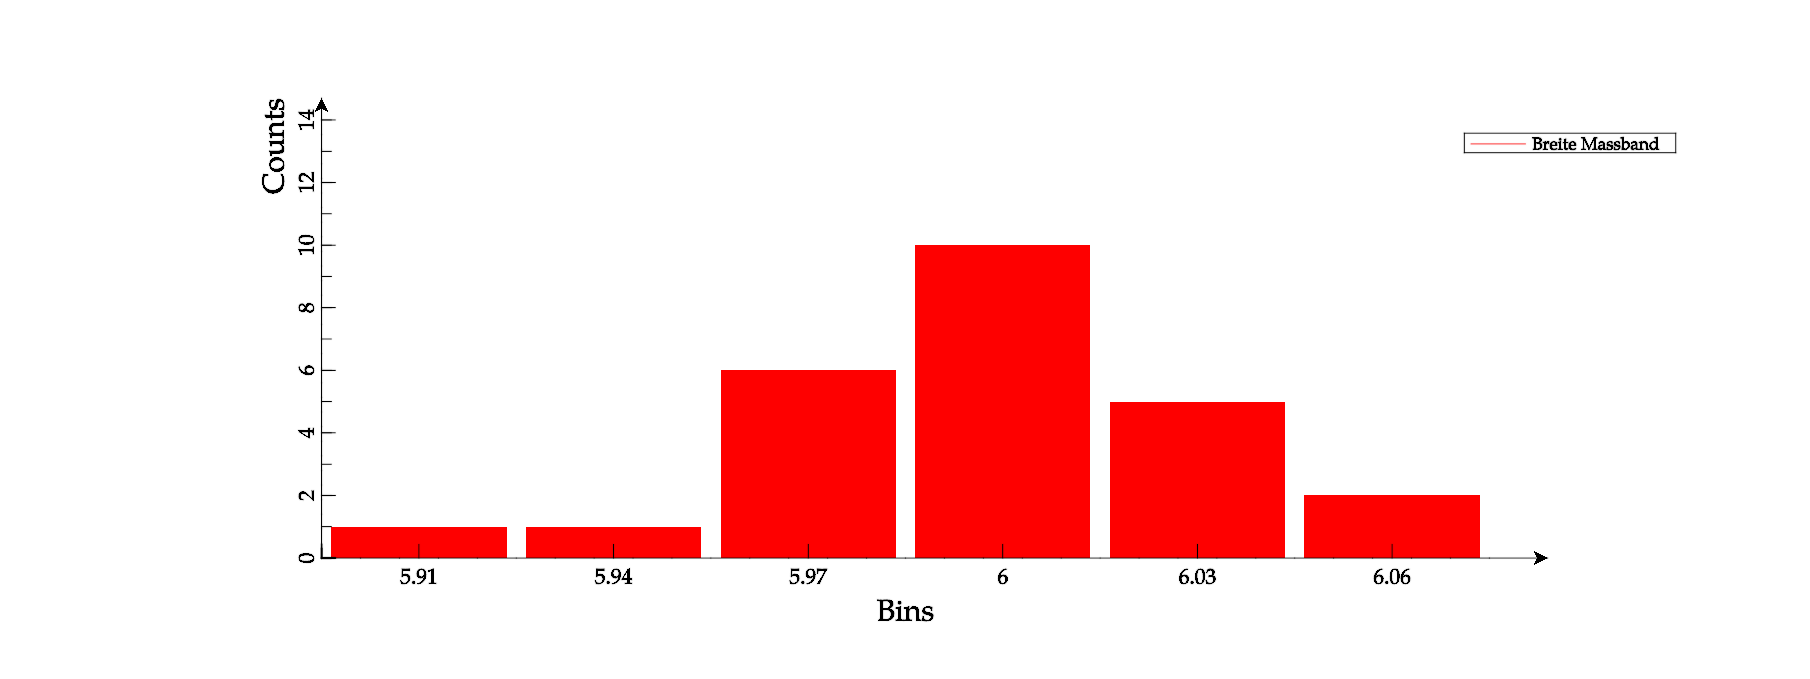
\includegraphics[width=\textwidth]{_graphics/histogramm.png}
					\caption{Histogramm eines Datensatzes erzeugt durch \texttt{hist}}
					\label{fig:histogramm}
				\end{figure}
				
				Histogramme der geladenen Daten erhält man durch \cmd{hist}
				\begin{lstlisting}
hist data(i1:i2,j1:j2)
				\end{lstlisting}
				Das Kommando \verb+hist+ unterstützt dabei eine große Zahl an Parametern, die das erzeugte Histogramm noch weiter beeinflussen können, aber bereits ohne Parameter werden gute Ergebnisse erzielt (\autoref{fig:histogramm}). Die Zahl der verwendeten Rubriken (auch \emph{bins}) wird durch die \emph{Sturges-Regel} bestimmt, kann aber auch direkt oder durch die \emph{Scott}- oder die \emph{Freedman-Diaconis-Regel} festgelegt werden.
				
				Es wird für jede Spalte eine Häufigkeitsanalyse durchgeführt und das Ergebnis in einem gemeinsamen Diagramm dargestellt. Spalten, die keine für eine Häufigkeitsanalyse sinnvollen Daten enthalten, sollten durch die Bereichssyntax ausgeschlossen werden.
				
				\NR\ kann auch Histogramme von zweidimensionalen Datensätzen anfertigen. Hierzu sind entweder die Option \verb+grid+ für ein einzelnes Histogramm oder das Kommando \cmd{hist2d}\verb+hist2d+ für Histogramme in zwei Raumrichtungen nötig. Details finden sich in dem entsprechenden Hilfeartikel.
				
				\helpidx{hist}
				Neben den Histogrammen und der Berechnung der Statistiken ist eine weitere, übliche Analysemethode durch das Anpassen einer Funktion (auch \emph{Modellkurve} oder \emph{Regressionsfunktion} genannt) an die gemessen (und ggf. zusätzlich aufbereiteten) Daten gegeben.
				
				Um eine Funktion \verb+FUNCTION()+ an Daten in \verb+data()+ anzupassen kann \verb+fit+ verwendet werden:\cmd{fit}
				\begin{lstlisting}
fit data(:,j1:j2) -with=FUNCTION(x,PARAMS) params=[PARAMS=INITIALW.]
fit data(:,1:2) -with=A*sin(B*x+C) params=[A=1,B=1,C=0]
				\end{lstlisting}
				\NR\ wird nun versuchen, die Parameter \verb+PARAMS+ so zu variieren, dass \verb+FUNCTION()+ die Datenpunkte möglichst treffend beschreibt. Die angepassten Werte werden in den Parametern hinterlegt, so dass mit diesen direkt weiter gerechnet werden kann. (In neueren \NR-Versionen ist \verb+params+ nicht mehr zwingend erforderlich, da die Parameter auch automatisch erkannt werden können.)
				
				Sobald \NR\ ein Minimum erreicht hat, bricht es den Algorithmus ab und gibt eine Übersicht aller Parameter aus, die im Folgenden beispielhaft dargestellt ist:
				\begin{verbatim}
					Funktion: 0.646875*sin(3.00223*x+0.00837336)
					Datenpunkte:                            101 ohne Gewichtungsfaktoren
					Freiheitsgrade:                         98
					Algorithmusparameter:                   TOL=0.0001, MAXITER=500
					Iterationen:                            7
					Gewichtete Summe der Residuen (chi^2):  2.33825
					Varianz der Residuen (red. chi^2):      0.0238597
					Standardabweichung der Residuen:        0.1544658

					Parameter  Initialwert      Anpassung    Asymptotischer Standardfehler
					----------------------------------------------------------------------
					A                    1      0.6468754    ± 0.02188576         (3.383%)
					B                    3       3.002228   ± 0.005649476        (0.1882%)
					C                    0    0.008373364    ± 0.06579646         (785.8%)
					----------------------------------------------------------------------

					Korrelationsmatrix der angepassten Parameter:

					/          1     0.0159    -0.0164 \
					|     0.0159          1     -0.862 |
					\    -0.0164     -0.862          1 /

					Fitanalyse:
					Die angepasste Funktion kann den Verlauf der Datenpunkte beschreiben,
					jedoch ist noch Raum für Optimierungen.
				\end{verbatim}
				Diese Übersicht enthält den bedeutenden $\chi^2$-Wert, der die Summe der quadratischen Abweichungen der Datenpunkten von der angepassten Funktion beschreibt. Außerdem finden sich hier die Ergebniswerte der Parameter und die berechneten Fehlerwerte, die in eine daraus erfolgende Fehlerfortpflanzung eingefügt werden können. Die Korrelationsmatrix der Parameter beschreibt, wie sehr die Parameter voneinander abhängen und die Fitanalyse fasst in Worte, was aus $\chi^2$ bzw. dem reduzierten $\chi^2$ herausgelesen werden kann. Diese Übersicht wird des Weiteren in \verb+<savepath>/numerefit.log+ protokolliert.
				\begin{figure}[htb]%
					\centering
					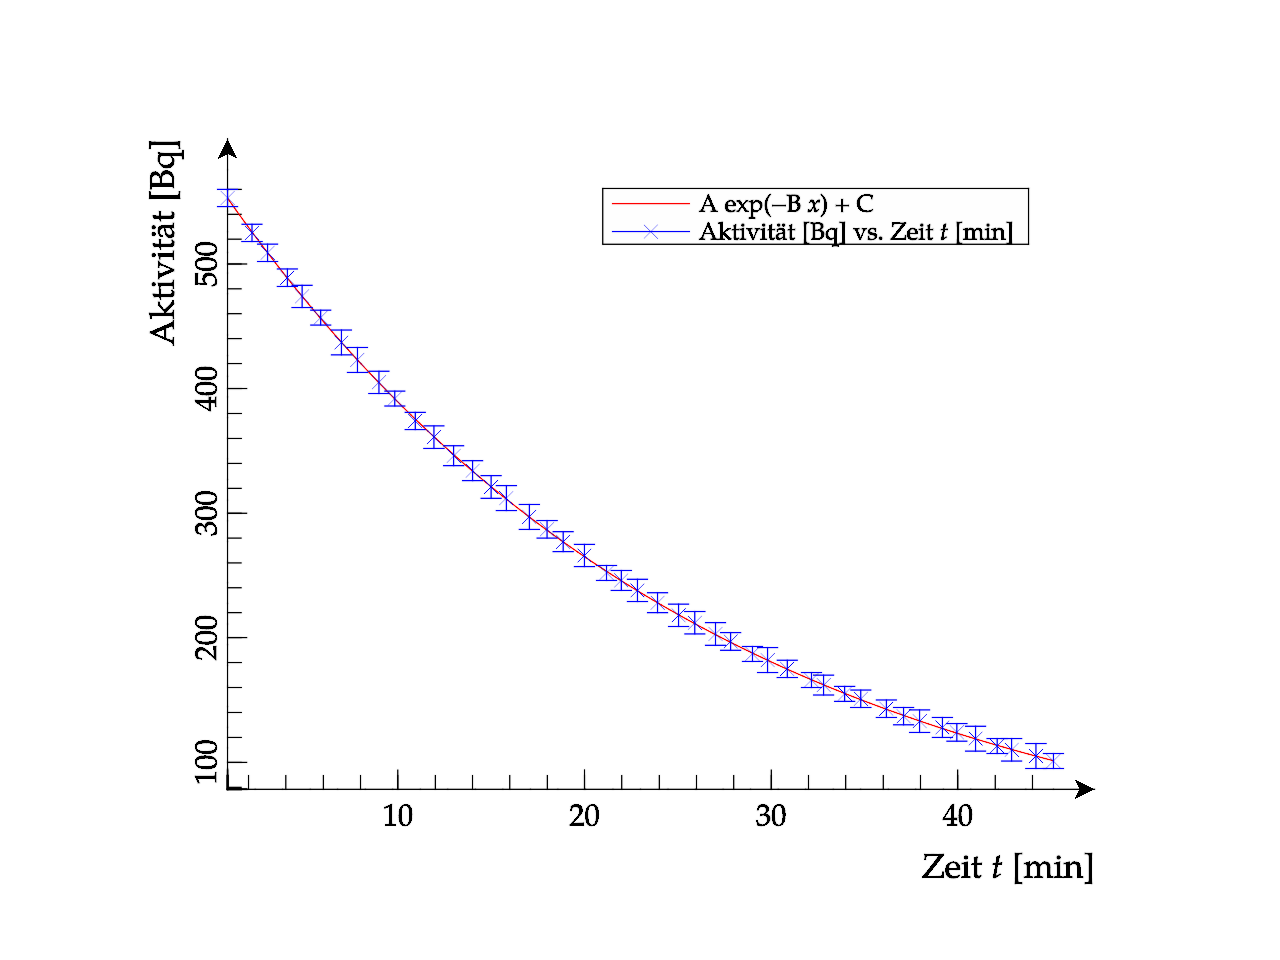
\includegraphics[width=\textwidth]{_graphics/plot.png}
					\caption{Anpassung des Modells eines exponentiellen Zerfalls an Messpunkte mittels \texttt{fitw}}
					\label{fig:fit}
				\end{figure}
				
				\paragraph{Anmerkung}
					Inwiefern der $\chi^2$-Wert eine Aussage über die Qualität einer Anpassung ist, ist eine Streitfrage. Im Allgemeinen nimmt man an, dass ein Fit mit einem möglichst kleinen $\chi^2$-Wert besonders gut ist. Genauer betrachtet ist die aussagekräftigere Größe der reduzierte $\chi^2$-Wert: für ihn gilt, dass wenn er deutlich kleiner als 1 ist, scheint die Anpassung gut zu treffen. Bei einem Fit, der Fehlerwerte berücksichtigt (s.u.), sollte dieser Wert jedoch möglichst nahe an 1 liegen. \NR\ berücksichtigt dies und liefert eine entsprechende Fitanalyse. Die Fitanalyse kann allerdings den optischen Vergleich von angepasster Funktion und Datenpunkten (siehe nächstes Kapitel) nicht ersetzen.\bigskip\\
				Im Anschluss an die Anpassung kann die angepasste Funktion zusammen mit den Daten mittels des Kommandos \verb+plot+ (siehe nächstes Kapitel) graphisch dargestellt werden (\autoref{fig:fit}). Dies bietet eine gute Möglichkeit, das Ergebnis der Anpassung zu überprüfen (und sollte eigentlich auch stets ausgeführt werden).
				
				Eine Anpassung an Datenpunkte, die mit Fehlern versehen sind, kann diese berücksichtigen. Dazu verwendet man\cmd{fitw}
				\begin{lstlisting}
fitw data(:,1:2:3) -with=A*sin(B*x+C) params=[A=1,B=1,C=0]
				\end{lstlisting}
				\verb+fitw+ (für \emph{weighted fit}) verwendet die Fehlerwerte in der dritten Spalte um die Datenpunkte entsprechend zu gewichten: Datenpunkte mit hohen Fehlern werden schwächer gewichtet als Datenpunkte mit geringen Fehlern.
				
				Sollte ein Fit mal nicht konvergieren, kann es helfen, die Initialwerte der Parameter (die stets angegeben werden sollten) selbst zu variieren. Ebenfalls kann es hilfreich sein, den Fitbereich einzugrenzen. Dies kann entweder durch eine Einschränkung der Zeilen in \verb+data()+ oder durch Übergabe der Option \verb+x=a:b+ erreicht werden:
				\begin{lstlisting}
fit data(:,1:2) -with=A*sin(B*x+C) params=[A=1,B=1,C=0] x=0:4
				\end{lstlisting}
				Zusätzlich können die Zahl der maximalen Iterationen, die Genauigkeit und einzuhaltende Bedingungen für die angegebenen Parameter vorgegeben werden. Letztere Option kann die Stabilität des Algorithmus allerdings drastisch beeinflussen.
				
				\helpidx{fit}
				Alle erwähnten Kommandos agieren spaltenweise. Falls die Daten zeilenweise vorliegen, muss man die folgende Zeile ausführen\cmd{copy}
				\begin{lstlisting}
copy data(:,:) -target=cache(:,:) transpose
				\end{lstlisting}
				und alle \verb+data+ in den vorherigen Beispielen durch \verb+cache+ ersetzen.
		\chapter{Erzeugen von Graphen}
			Eine besonders wichtige Funktionalität von \NR\ ist die Erzeugung von Funktions- und Datengraphen. Hiermit können die Verläufe von Funktionen und Daten visualisiert und damit einfacher analysiert werden. \NR\ gibt alle generierten Darstellungen automatisch als Bildatei aus. Wenn \NR\ mit einem Bildbetrachter verknüpft ist, wird dieser im Anschluss an den \emph{Plotvorgang} automatisch mit der Bilddatei gestartet.
			\section{Typen von Graphen}
				\NR\ kennt eine große Zahl unterschiedlicher Plotarten, die durch die Angabe weiterer Plotoptionen noch auf unzählige weitere Arten modifiziert werden können. Hier sollen nur die wichtigsten aufgezählt werden, der komplette Satz an Plottypen ist unter \verb+list -cmd+ zu finden:
				\begin{lstlisting}
plot
plot3d
mesh
dens
vect
vect3d
...
				\end{lstlisting}
				\begin{itemize}
					\item \verb+plot+: dies erzeugt einen Standardgraphen, bei dem $y$ gegen $x$ aufgetragen ist. Dieses Kommando wird verwendet, um z.B. $\sin x$ oder $x^2$ graphisch darzustellen.
					\item \verb+plot3d+: dieses Kommando generiert einen Graphen auf Basis einer 3D-Trajektorie. Aus drei Funktionen mit der Variable $t$ wird eine Bahnkurve berechnet und diese dreidimensional dargestellt.
					\item \verb+mesh+: eine Funktion $z = f(x,y)$ kann mit diesem Kommando dargestellt werden. Es wird ein Gitterplot berechnet und dreidimensional dargestellt.
					\item \verb+dens+: im Gegensatz zu \verb+mesh+ stellt dieses Kommando die Funktion $z = f(x,y)$ nur durch reine Farbwerte als Projektion auf die $x$-$y$-Ebene dar.
					\item \verb+vect+: dieser Plotstil berechnet einen Vektorplot eines 2D-Vektorfeldes: $\vec A(x,y) = A_x(x,y)\,\hat e_x + A_y(x,y)\,\hat e_y$.
					\item \verb+vect3d+: ähnlich wie \verb+vect+ berechnet dies einen Vektorplot, allerdings den eines dreidimensionalen Vektorfeldes: $\vec A(x,y,z) = A_x(x,y,z)\,\hat e_x + A_y(x,y,z)\,\hat e_y + A_z(x,y,z)\,\hat e_z$.
				\end{itemize}
			\section{Ausgabeformate}
				Das standardmäßige Ausgabeformat für Plots ist eine Bilddatei im PNG-Format im Verzeichnis \verb+<plotpath>+ (Dies ist standardmäßig der Unterorder ">plots"< im \NR-Stammverzeichnis). Die Bilddatei wird dabei automatisch entsprechend des Plotkommandos benannt. Mit den Plotoptionen \verb+opng+, \verb+oeps+, \verb+ogif+, \verb+osvg+ und \verb+otex+ sind auch weitere Ausgabeformate und andere Dateinamen möglich.
				
				Um einen einfachen Plot in z.B. ">graph\_der\_messung.png"< zu erzeugen, ist die Option
				\begin{lstlisting}
opng=graph_der_messung
				\end{lstlisting}
				zu übergeben. Sollte der Dateiname Leerzeichen enthalten, muss dieser in Anführungszeichen angegeben werden.
				
				\helpidx{plotoptions}
			\section{Verwendung}
				Alle Plotbefehle folgen in ihrer Syntax dem folgenden Schema:
				\begin{lstlisting}
KOMMANDO FUNKTIONEN/DATEN -set OPTIONEN
				\end{lstlisting}
				wobei die \verb+OPTIONEN+ optional sind und nicht angegeben werden müssen.
				
				Standardvariablen sind $x, y, z$ und $t$. Je nach Plotkommando wird eine, zwei, drei oder alle vier dieser Variablen als Variablen verwendet und die restlichen als Parameter betrachtet. \verb+plot+ verwendet nur $x$, \verb+plot3d+ nur $t$, \verb+mesh+, \verb+dens+ und \verb+vect+ $x$ und $y$ und \verb+vect3d+ $x,y$ und $z$. Alle anderen Variablen werden als Parameter betrachtet.
				
				Ein einfacher Sinus-Plot wird durch\cmd{plot}
				\begin{lstlisting}
plot sin(x)
				\end{lstlisting}
				erreicht. Hier wird automatisch ein Achsenkreuz und ein Sinus von $-10$ bis 10 berechnet, wobei die $y$-Achse passend, jedoch ein kleines Stück größer gewählt wird. Die Achsenbeschriftung und die Legende wird ebenfalls selbstständig bestimmt (\autoref{fig:sinusplots}a)
				\begin{figure}[p]%
					\centering
					\subfloat[ohne Optionen]{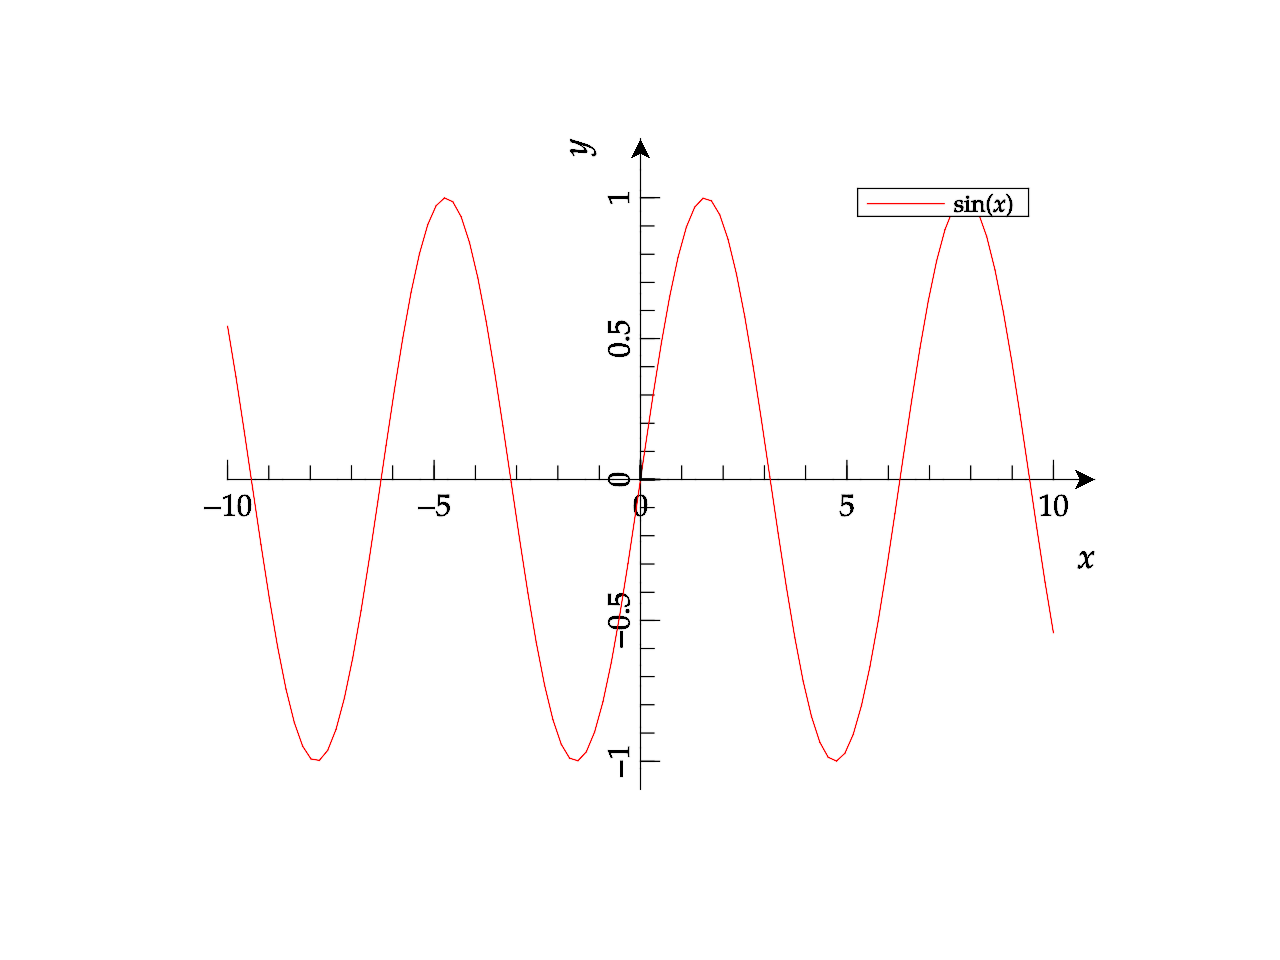
\includegraphics[width=0.45\textwidth]{_graphics/plot_0.png}}
					\subfloat[mit \texttt{box} und \texttt{grid}]{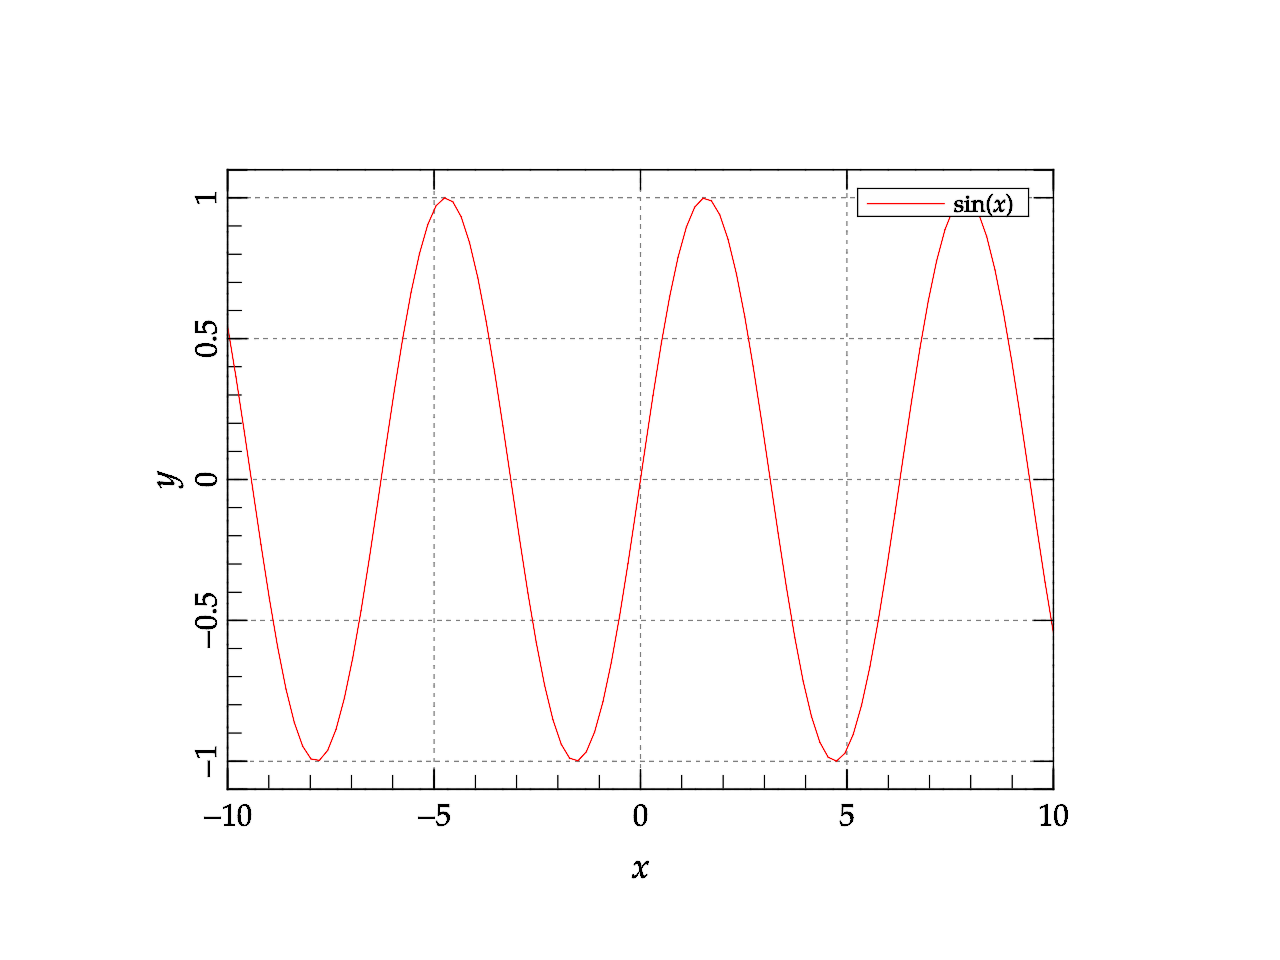
\includegraphics[width=0.45\textwidth]{_graphics/plot_1.png}}\\
					\subfloat[mit eigener Legende]{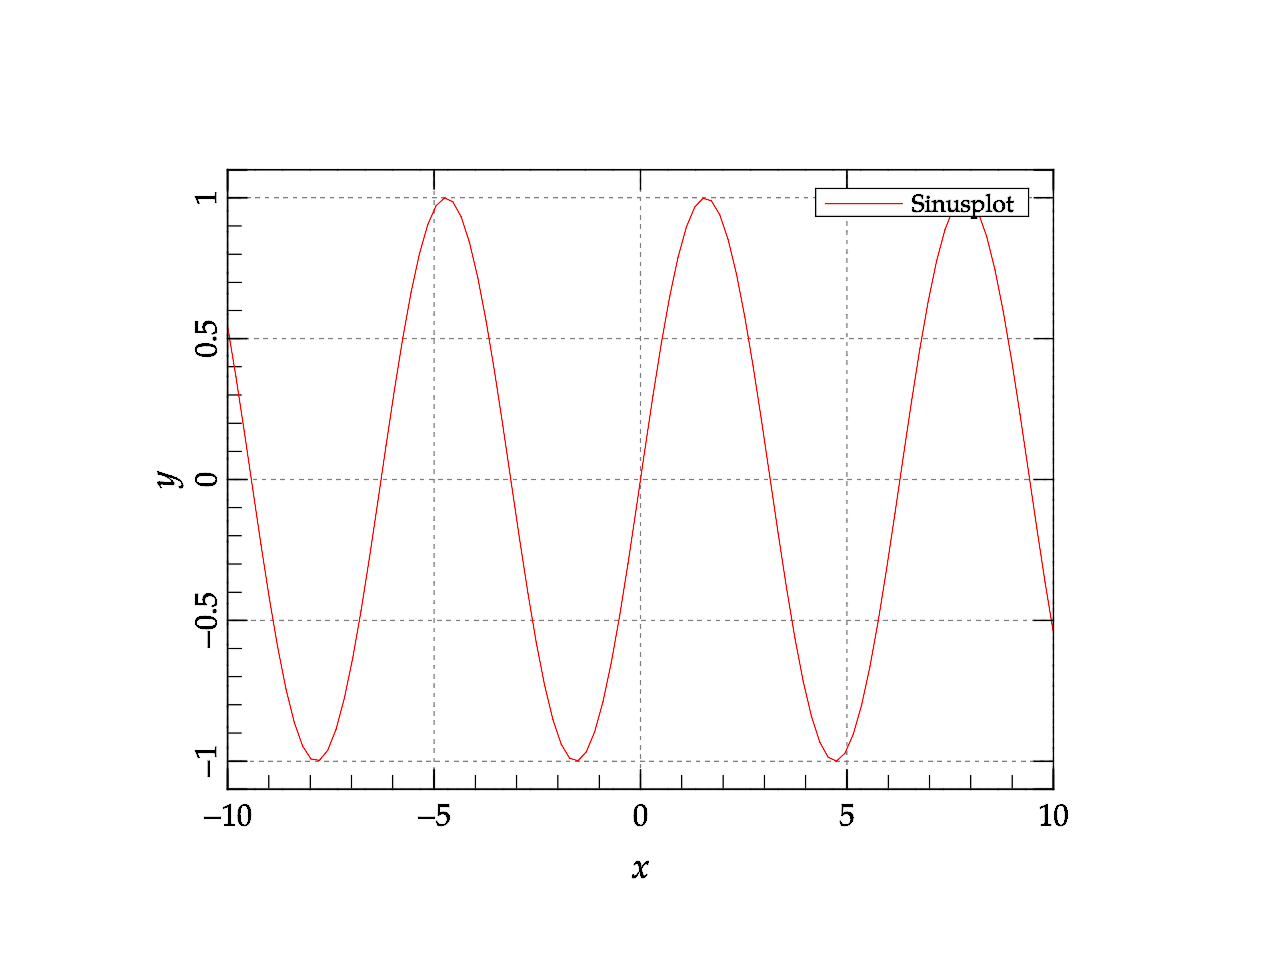
\includegraphics[width=0.45\textwidth]{_graphics/plot_2.png}}
					\subfloat[mit Datensatz]{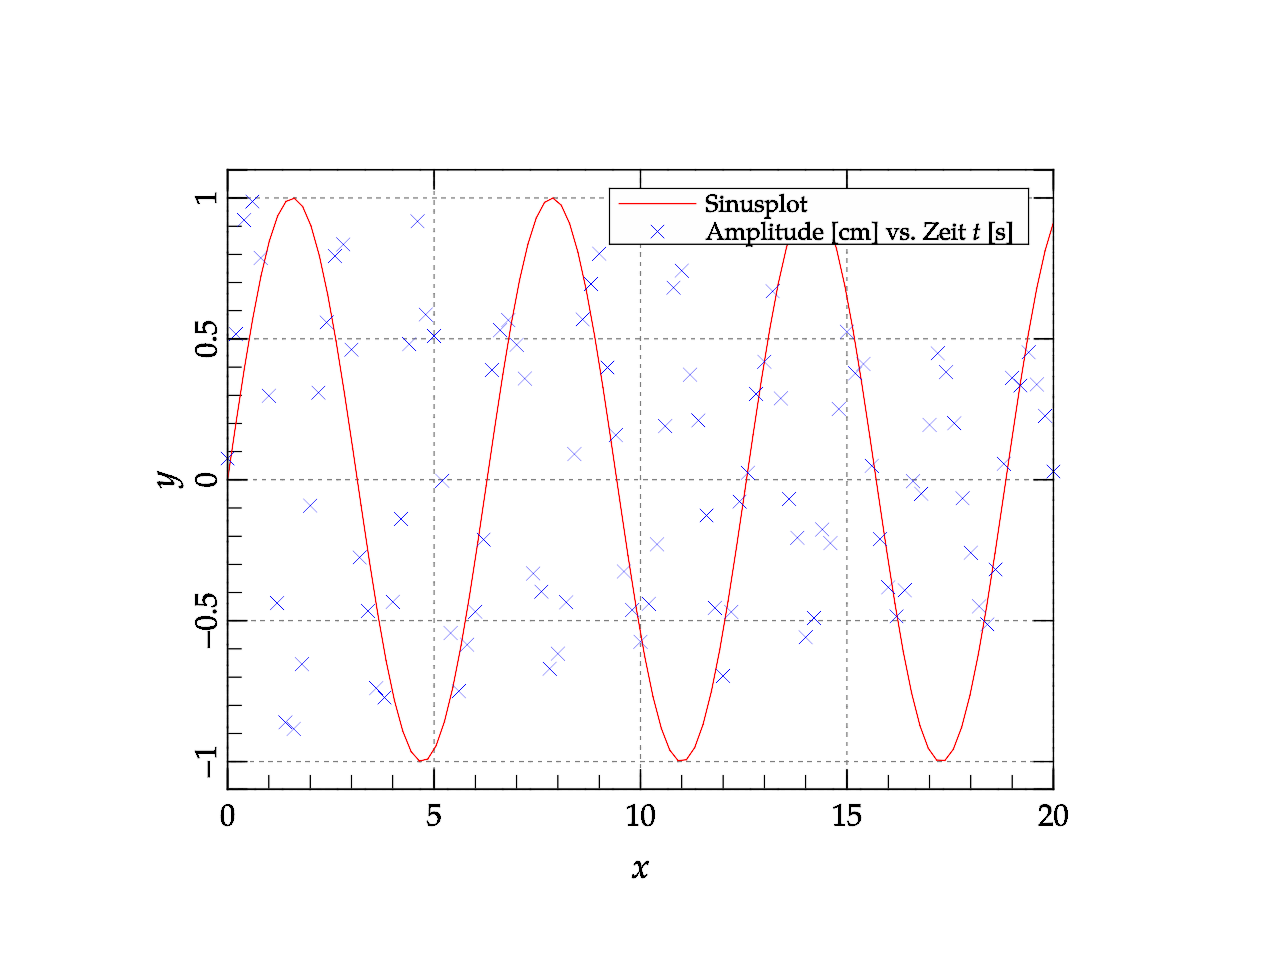
\includegraphics[width=0.45\textwidth]{_graphics/plot_3.png}}\\
					\subfloat[mit eigenen Intervallgrenzen]{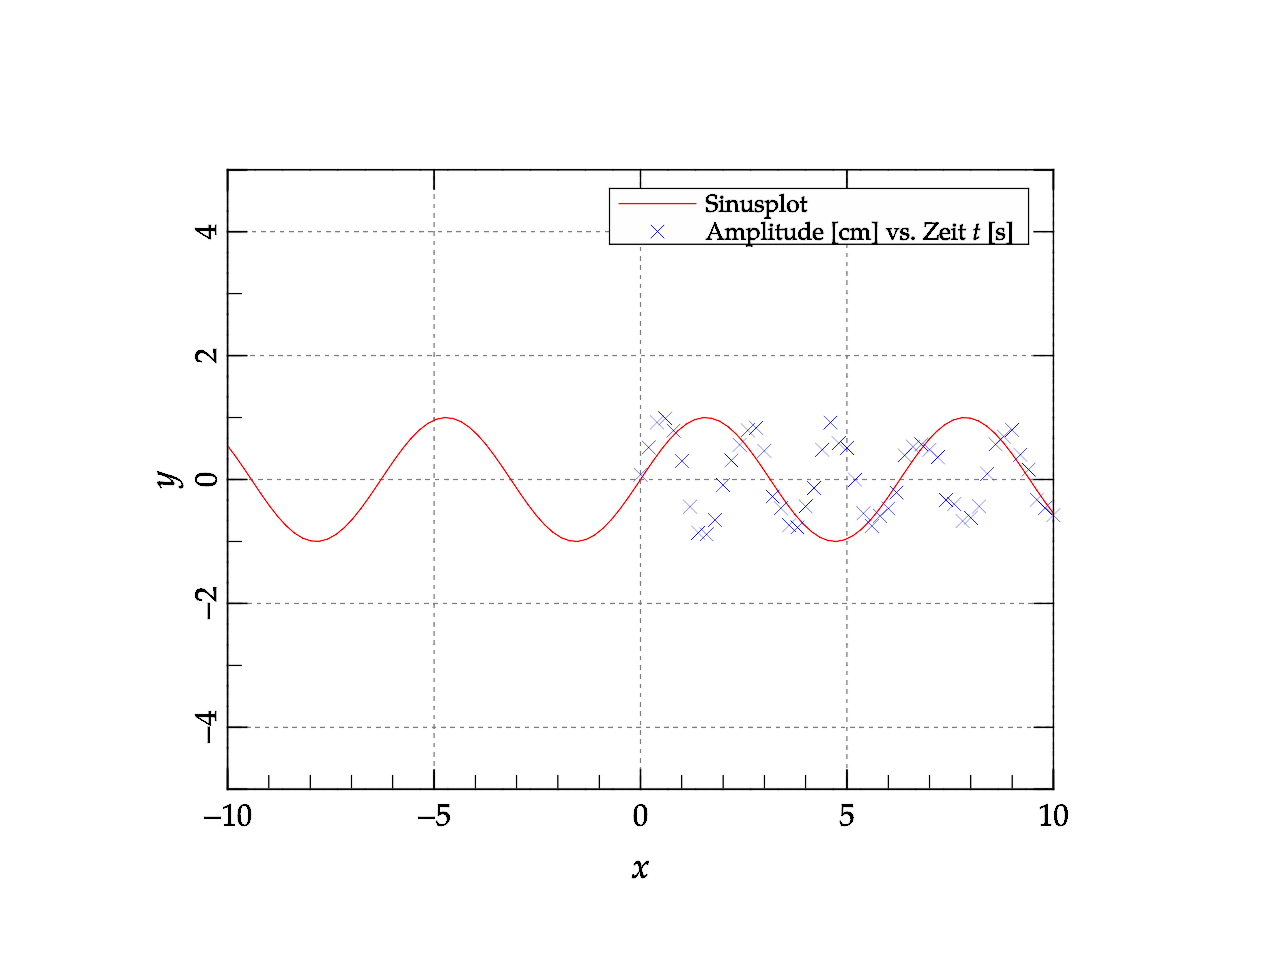
\includegraphics[width=0.45\textwidth]{_graphics/plot_4.png}}
					\subfloat[mit Fehlerbalken]{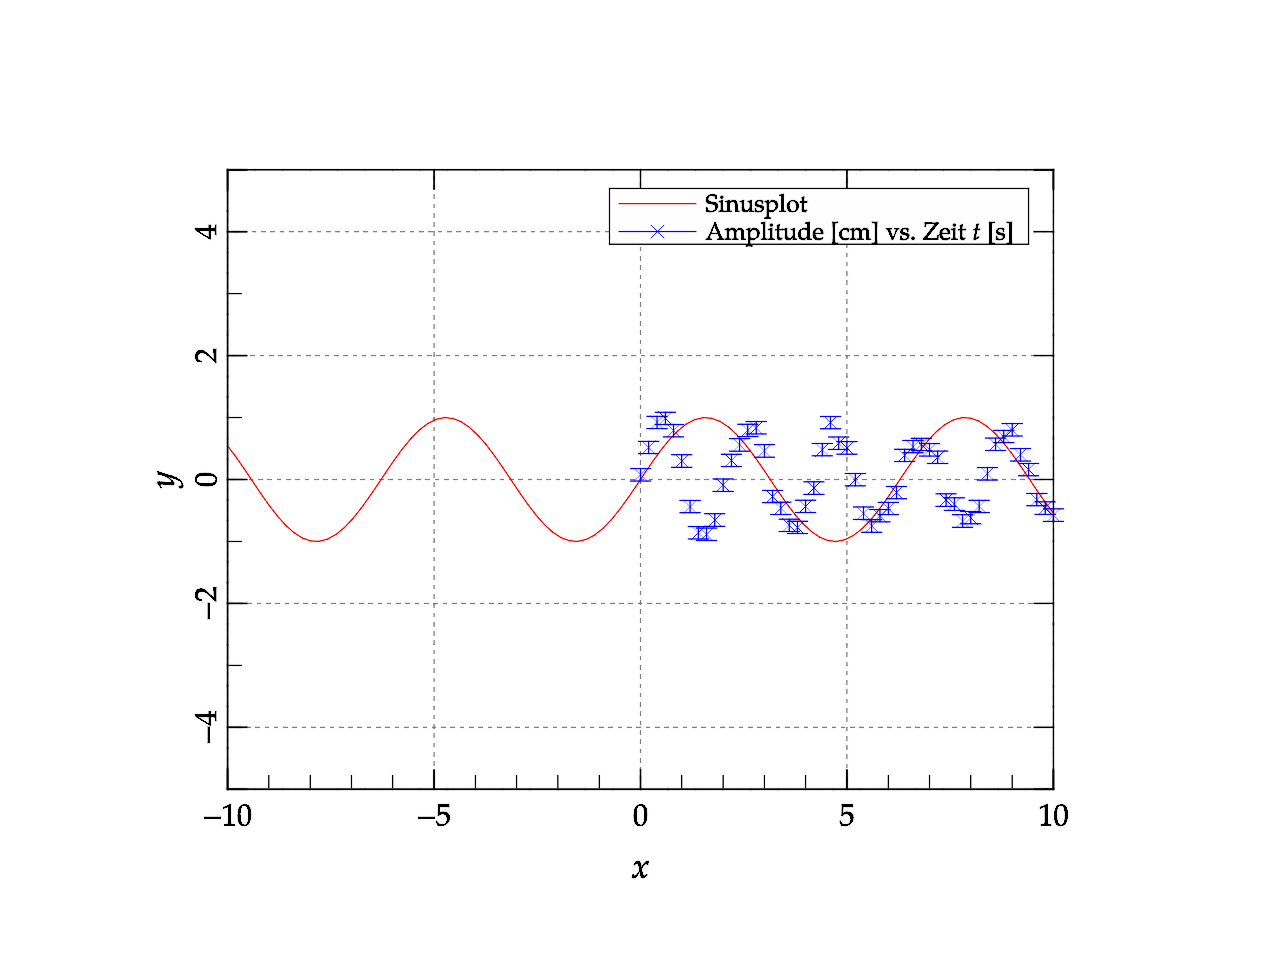
\includegraphics[width=0.45\textwidth]{_graphics/plot_5.png}}
					\caption{Die Ergebnisgraphen unter Verwendung der gezeigten Optionen}
					\label{fig:sinusplots}
				\end{figure}
				
				\helpidx{plot}
				Eine umfassende Box und ein Koordinatengitter wird erreicht durch
				\begin{lstlisting}
plot sin(x) -set box grid
				\end{lstlisting}
				Ab diesem Plot werden alle folgenden Plots ebenfalls mit Gitter und umfassender Box ausgestattet (\autoref{fig:sinusplots}b und c).
				
				Möchte man außerdem noch ">Sinusfunktion"< statt ">$\sin(x)$"< als Legende haben, gibt man folgendes an:
				\begin{lstlisting}
plot sin(x) "Sinusfunktion" -set box grid
				\end{lstlisting}
				(\autoref{fig:sinusplots}c; Eine leere Legende erreicht man durch Angabe einer leeren Zeichenkette \verb+""+)
				
				\NR\ kann auch Datensätze graphisch darstellen. Dazu gibt man den Datensatz in \verb+data()+ analog zu einer Funktion an. Bleibt die Argumentklammer leer, wird dies automatisch durch \verb+data(:,:)+ ersetzt. Es können aber auch direkt die nötigen Spalten angegeben werden, z.B. \verb+data(:,1:4)+. Dies verwendet entweder Spalte 1 und 4 oder Spalte 1 bis 4, falls der entsprechende Plotstil mehr als zwei Spalten benötigt. Es können hierbei bis zu 6 einzelne Spalten in beliebiger Reihenfolge angegeben werden: \verb+data(:,4:2:6:1:3:8)+.
				
				In Verbindung mit dem vorherigen Beispiel könnte man Spalten 1 und 2 und den Sinus zusammen durch
				\begin{lstlisting}
plot sin(x) "Sinusfunktion", data() -set box grid
				\end{lstlisting}
				darstellen (\autoref{fig:sinusplots}d). Auch für \verb+data()+ kann eine eigene Legende angegeben werden. Anderenfalls wird eine Kombination aus den Spaltentiteln verwendet. Interessant ist des Weiteren, dass mit Einbringen des Datensatzes die $x$-Achse passend zum Datensatz gewählt wird und nicht mehr zwangsläufig von $-10$ bis 10 verläuft. Dazu wird auffallen, dass die \NR\ Datenpunkte als einzelne Punkte darstellt und sie nicht durch eine (unphysikalische) Linie verbindet.
				
				Die Plotintervalle können für einen Plot global überschrieben werden, wenn sie explizit angegeben werden:
				\begin{lstlisting}
plot sin(x) "Sinusfunktion", data() -set box grid [-10:10,-5:5]
				\end{lstlisting}
				Dies erzeugt einen Graphen mit dem $x$-Intervall $[-10;10]$ und dem $y$-Intervall $[-5;5]$ (\autoref{fig:sinusplots}e). Diese Option wird \emph{nicht} für alle folgenden Plots übernommen.
				
				Messungen von Datenpunkten sind in vielen Fällen mit Fehlern belastet. Sind diese bekannt, so kann \NR\ diese auch darstellen. Sind nur die $y$-Werte mit Fehlern behaftet, so benötigt \NR\ drei Spalten ($x,y,\Delta y$), bei Fehlern in beide Richtungen sind es vier ($x,y,\Delta x, \Delta y$). Die dazu nötige Plotoption heißt \verb+errorbars+ bzw. \verb+yerrorbars+, wenn nur $y$-Fehler vorhanden sind.
				
				Nehmen wir nun an, dass die Datenpunkte in obigem Beispiel mit $y$-Fehlern behaftet sind:
				\begin{lstlisting}
plot sin(x) "Sinusfunktion", data() -set box grid [-10:10,-5:5] yerrorbars
				\end{lstlisting}
				Es erscheinen Fehlerbalken in $y$-Richtung, obwohl die Angabe der Spaltenzahl nicht geändert wurde! \NR\ interpretiert die leere Argumentklammer nun automatisch um und verwendet die ersten drei Spalten (\autoref{fig:sinusplots}f).
				
				\helpidx{plotoptions}
				\cmd{mesh}In einem anderen Fall soll eine zweidimensionale Funktion durch ein Gitterplot dargestellt werden: ein Sinus Cardinalis von $\varrho$ ($\text{sinc}\,\varrho$):
				\begin{lstlisting}
mesh sinc(norm(x,y))
				\end{lstlisting}
				\begin{figure}[p]%
					\centering
					\subfloat[nur \texttt{mesh}]{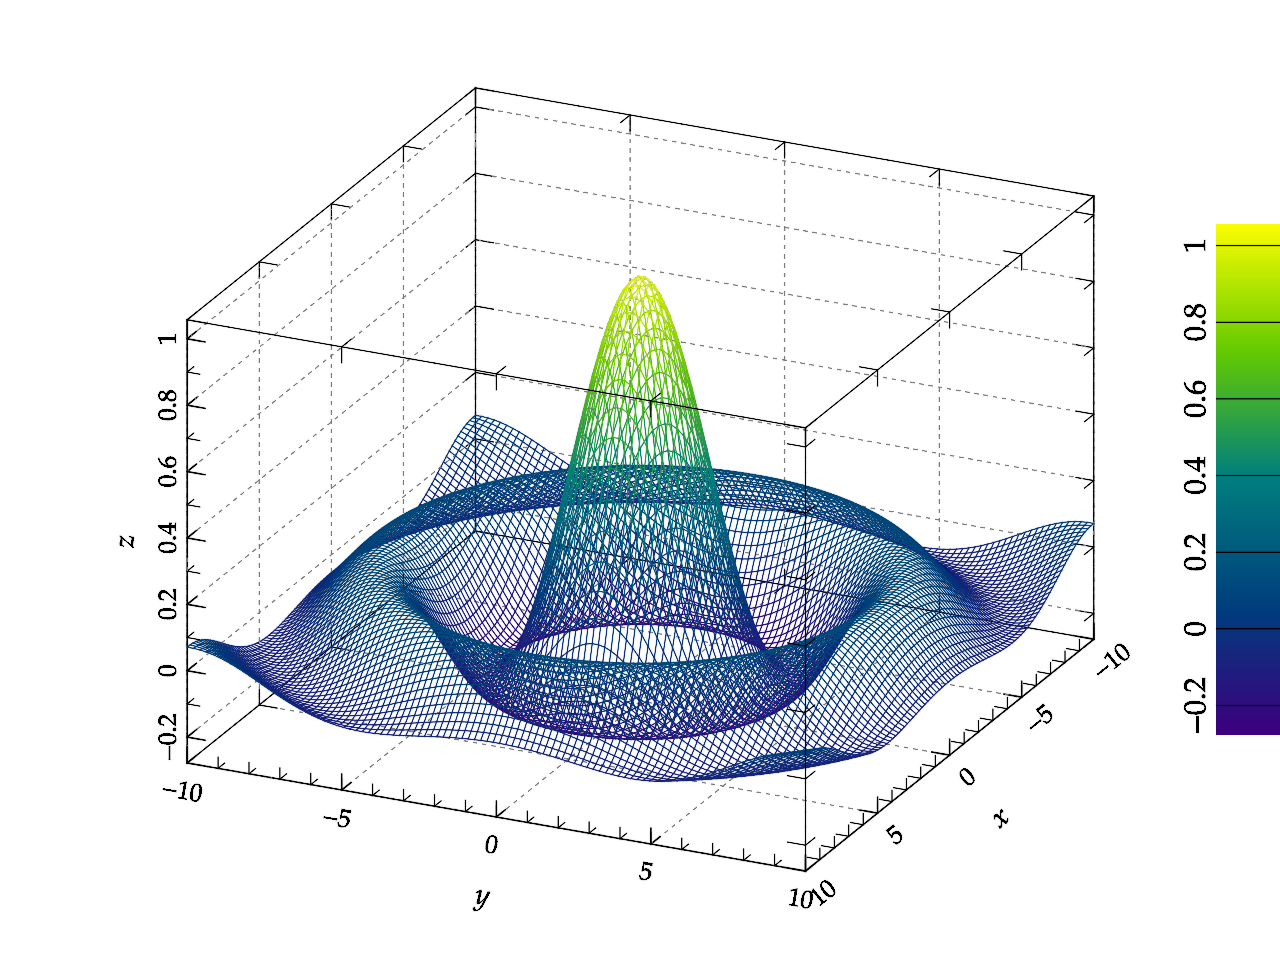
\includegraphics[width=0.45\textwidth]{_graphics/mesh_0.png}}
					\subfloat[mit \texttt{nobox}]{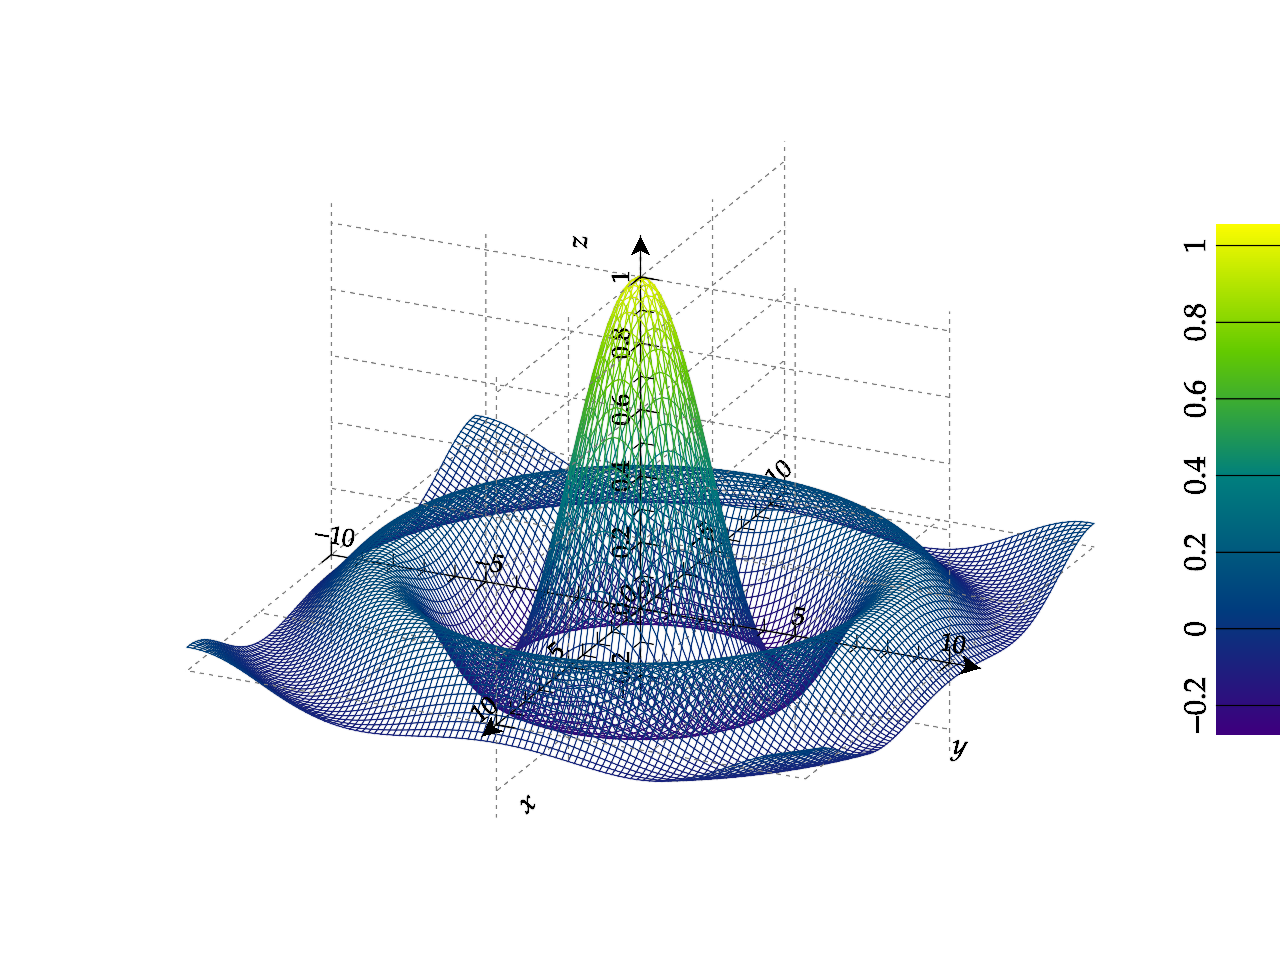
\includegraphics[width=0.45\textwidth]{_graphics/mesh_1.png}}\\
					\subfloat[mit \texttt{rotate}]{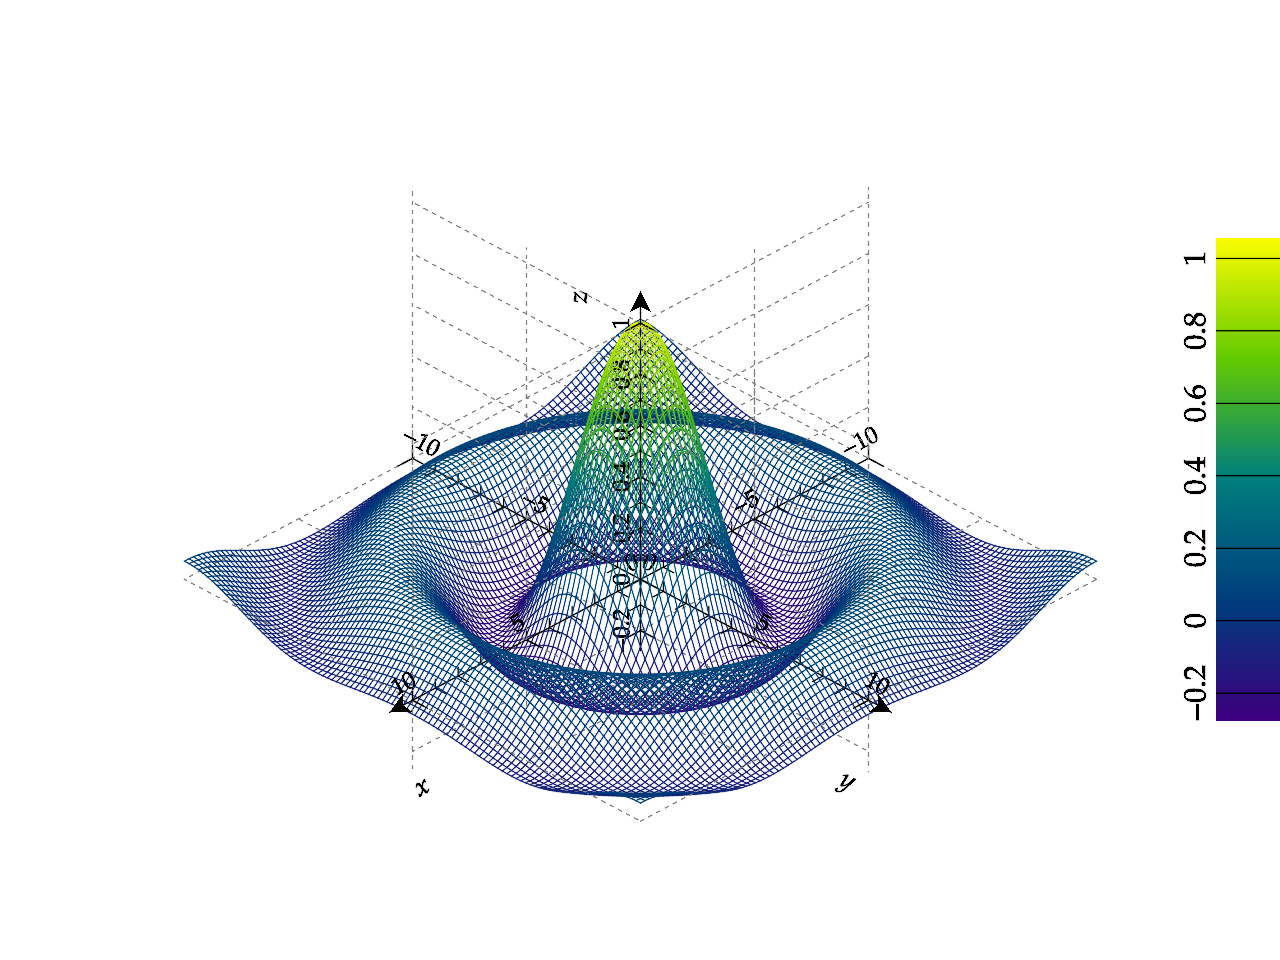
\includegraphics[width=0.45\textwidth]{_graphics/mesh_2.png}}\\
					\subfloat[nur \texttt{vect}]{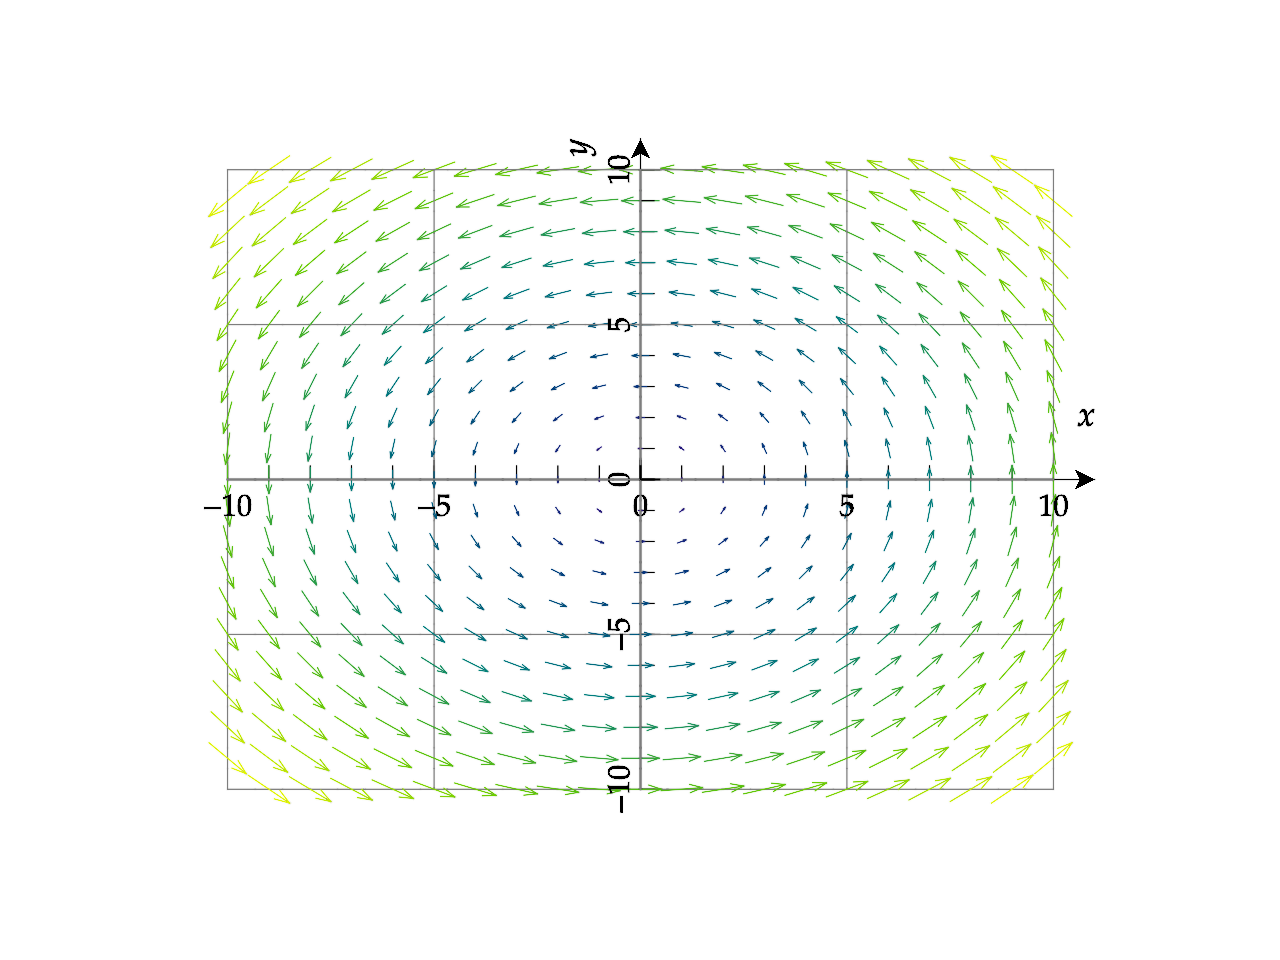
\includegraphics[width=0.45\textwidth]{_graphics/vect_0.png}}
					\subfloat[mit \texttt{flength}]{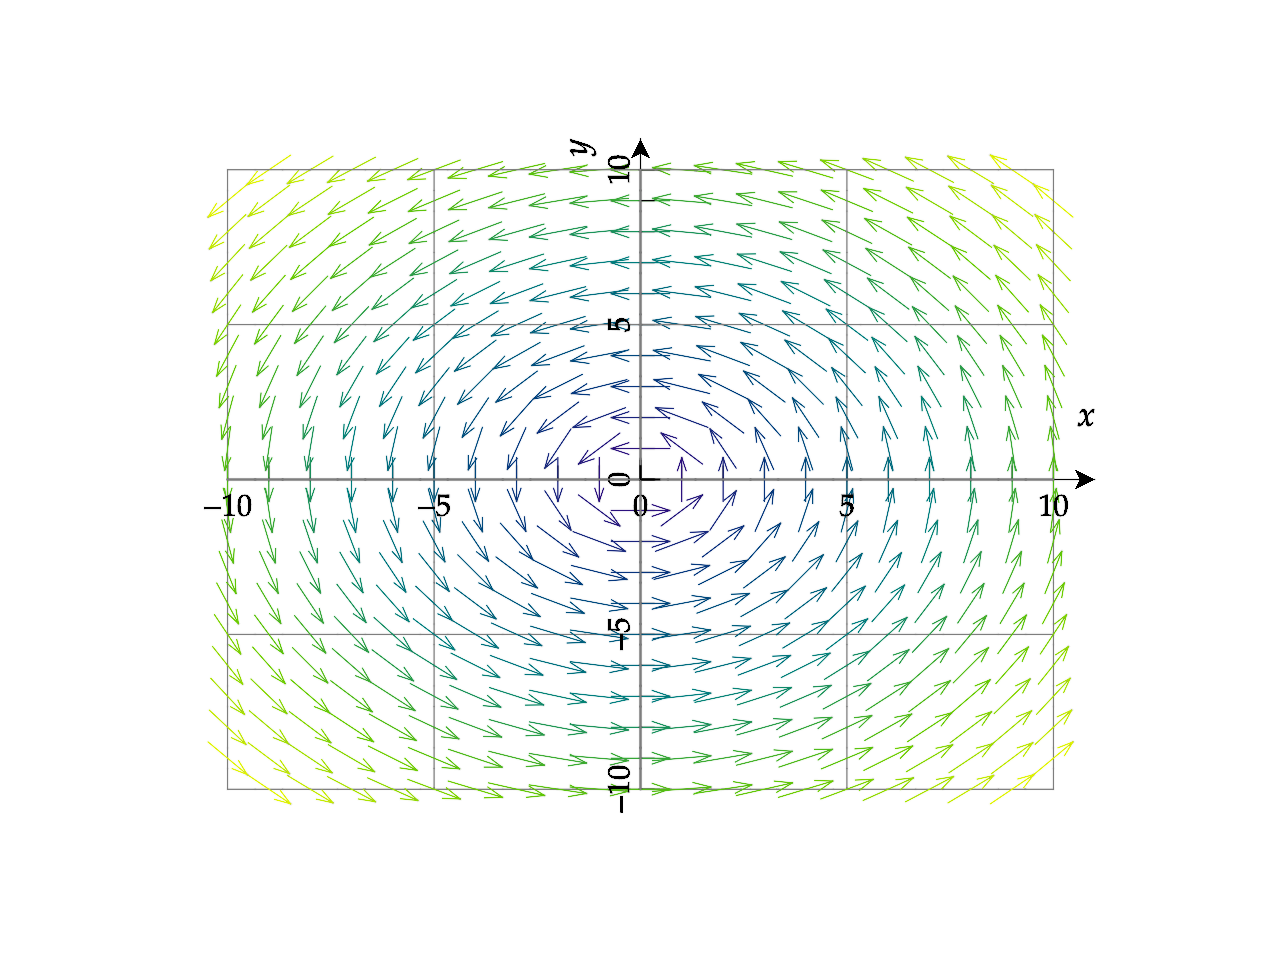
\includegraphics[width=0.45\textwidth]{_graphics/vect_1.png}}
					\caption{Ergebnisse der Gitter- und Vektorplots}
					\label{fig:mesh_vect}
				\end{figure}
				\verb+mesh+ erzeugt den gewünschten Gitterplot (\autoref{fig:mesh_vect}a). Die Funktion \verb+norm()+ ist die $n$-dimensionale, euklidische Vektornorm (diese Funktion kann beliebig viele Argumente aufnehmen):
				\begin{equation*}
					\text{norm}(x,y,z,\ldots) := \sqrt{x^2+y^2+z^2+\ldots}
				\end{equation*}
				Für diesen Fall beschreibt $\text{norm}(x,y) = \varrho$. Direkt im Anschluss an den vorherigen Plot ausgeführt sollte auffallen, dass auch der Gitterplot von einer umfassenden Box umgeben und ein Gitter im Hintergrund zeigt. Um die Box zu entfernen, gibt man \verb+nobox+ an (\autoref{fig:mesh_vect}b):
				\begin{lstlisting}
mesh sinc(norm(x,y)) -set nobox
				\end{lstlisting}
				
				Der Gitterplot ist automatisch auf eine bestimmte Ausrichtung gedreht. Dies kann auch geändert werden:
				\begin{lstlisting}
mesh sinc(norm(x,y)) -set rotate=45,135
				\end{lstlisting}
				Der Graph erscheint nun etwas mehr gekippt und auch die $x$- und $y$-Achsen erscheinen symmetrisch zu beiden Seiten (\autoref{fig:mesh_vect}c). Tatsächlich wurde der Graph mit diesen Werten in Richtung der ersten Raumdiagonale gedreht. Die Winkelwerte von \verb+rotate+ sind in Grad angegeben und zwar in der Reihenfolge $\vartheta,\varphi$, wobei $\vartheta$ den Graphen kippt und $\varphi$ ihn rotiert.
				
				\helpidx{mesh}
				Ein weiteres Beispiel soll der Vektorplot eines 2D-Rotationsfeldes sein:
				\[\vec A(x,y) = 2\svec{-y\\x}\]
				Dies erreicht man durch\cmd{vect}
				\begin{lstlisting}
vect -2*y,2*x
				\end{lstlisting}
				Hier wird die erste Funktion als Amplitude in $\hat e_x$-Richtung und die zweite Funktion in $\hat e_y$-Richtung interpretiert (\autoref{fig:mesh_vect}d). Zwecks der Übersicht akzeptiert \verb+vect+ (und \verb+vect3d+) nur ein Vektorfeld.
				
				Die Länge der Vektorpfeile entspricht der lokalen Amplitude des Vektorfeldes. Um diesen Effekt zu deaktivieren, kann 
				\begin{lstlisting}
vect -2*y,2*x -set flength
				\end{lstlisting}
				angegeben werden (\autoref{fig:mesh_vect}e).
				
				\helpidx{vect}
			\section{Koordinatensysteme}
				Zuletzt soll an dieser Stelle noch auf die unterschiedlichen Koordinatensysteme eingegangen werden. \NR\ unterstützt drei verschiedene Koordinatensysteme: das \emph{kartesische}, das \emph{polare} oder \emph{zylindrische} und das \emph{sphärische}.
				\begin{figure}[htb]%
					\centering
					\subfloat[\texttt{plot} mit \texttt{coords=polar}]{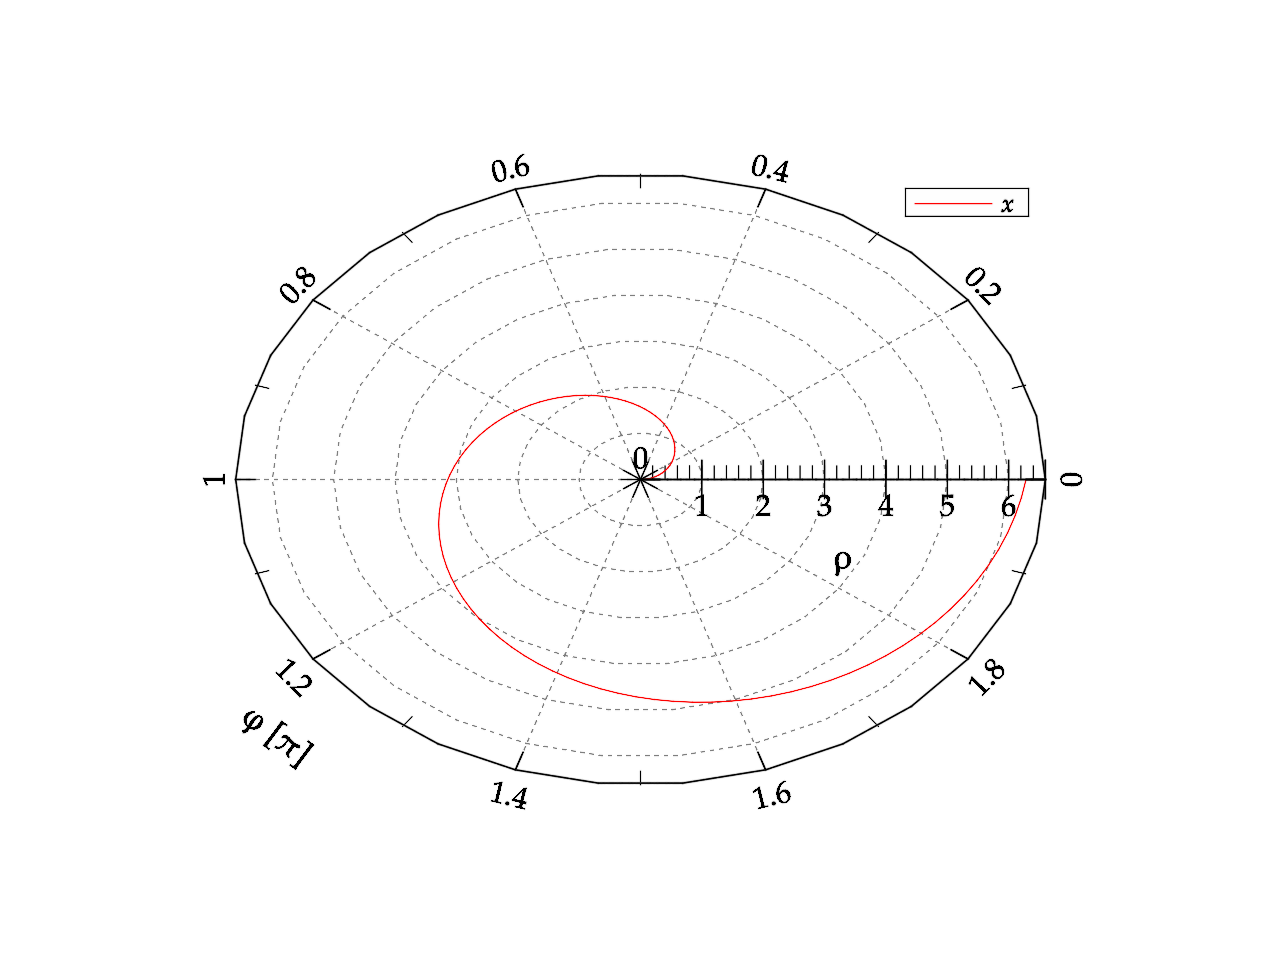
\includegraphics[width=0.45\textwidth]{_graphics/plot_6.png}}
					\subfloat[mit größerem Intervall]{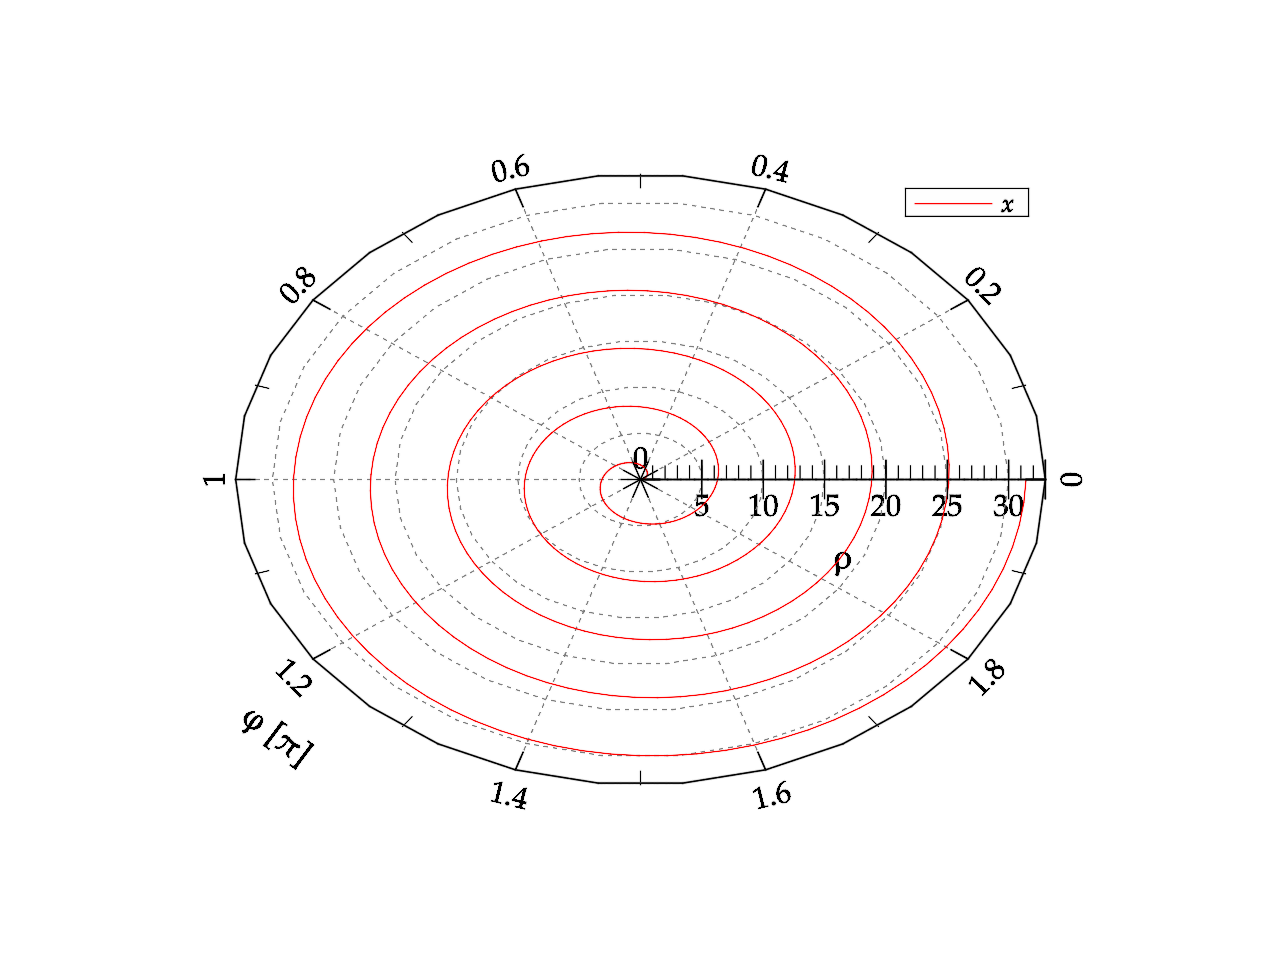
\includegraphics[width=0.45\textwidth]{_graphics/plot_7.png}}\\
					\subfloat[\texttt{surf} mit \texttt{light}]{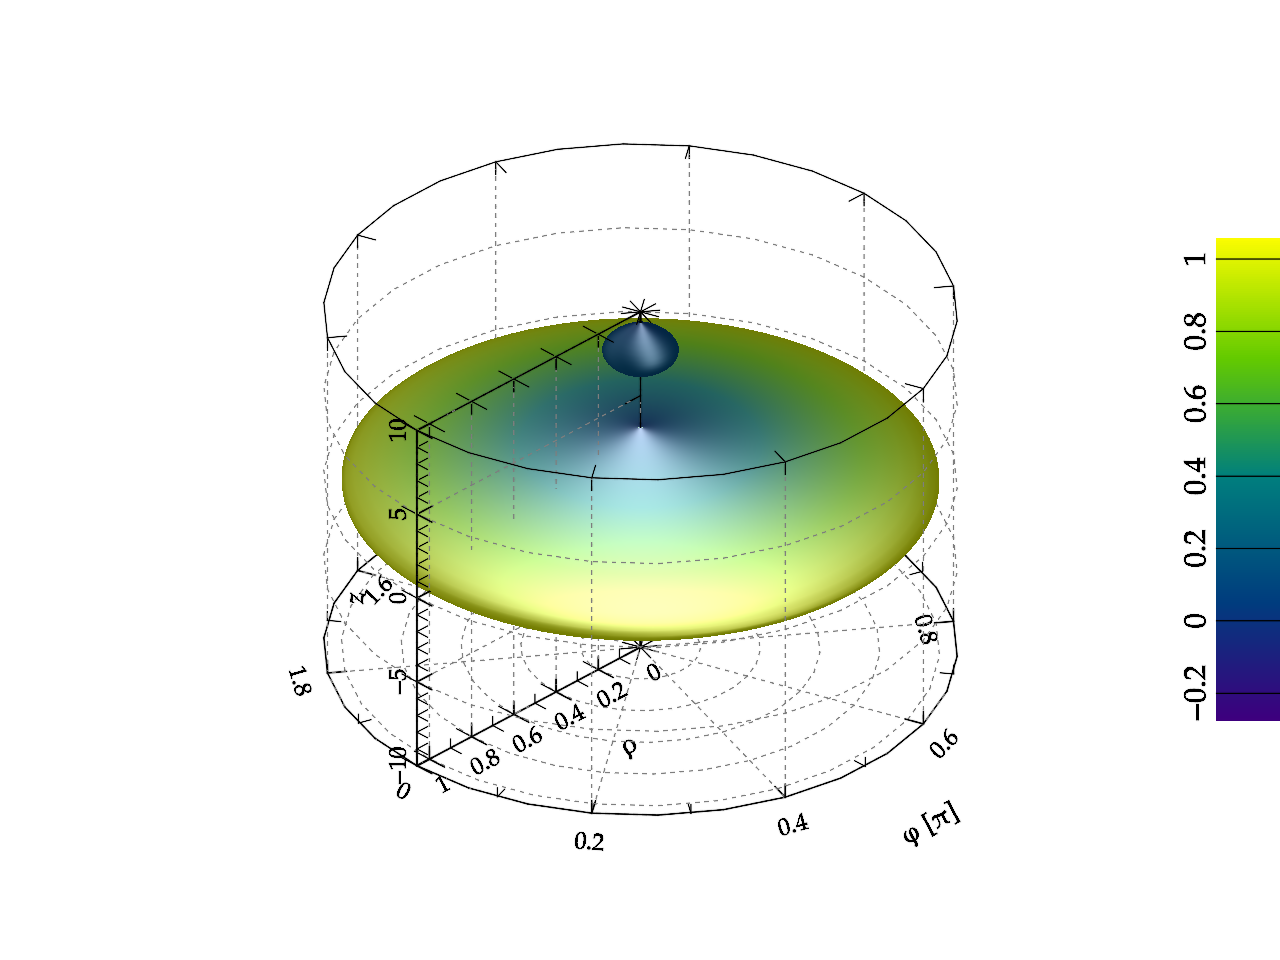
\includegraphics[width=0.45\textwidth]{_graphics/surf_0.png}}
					\subfloat[mit \texttt{coords=spherical}]{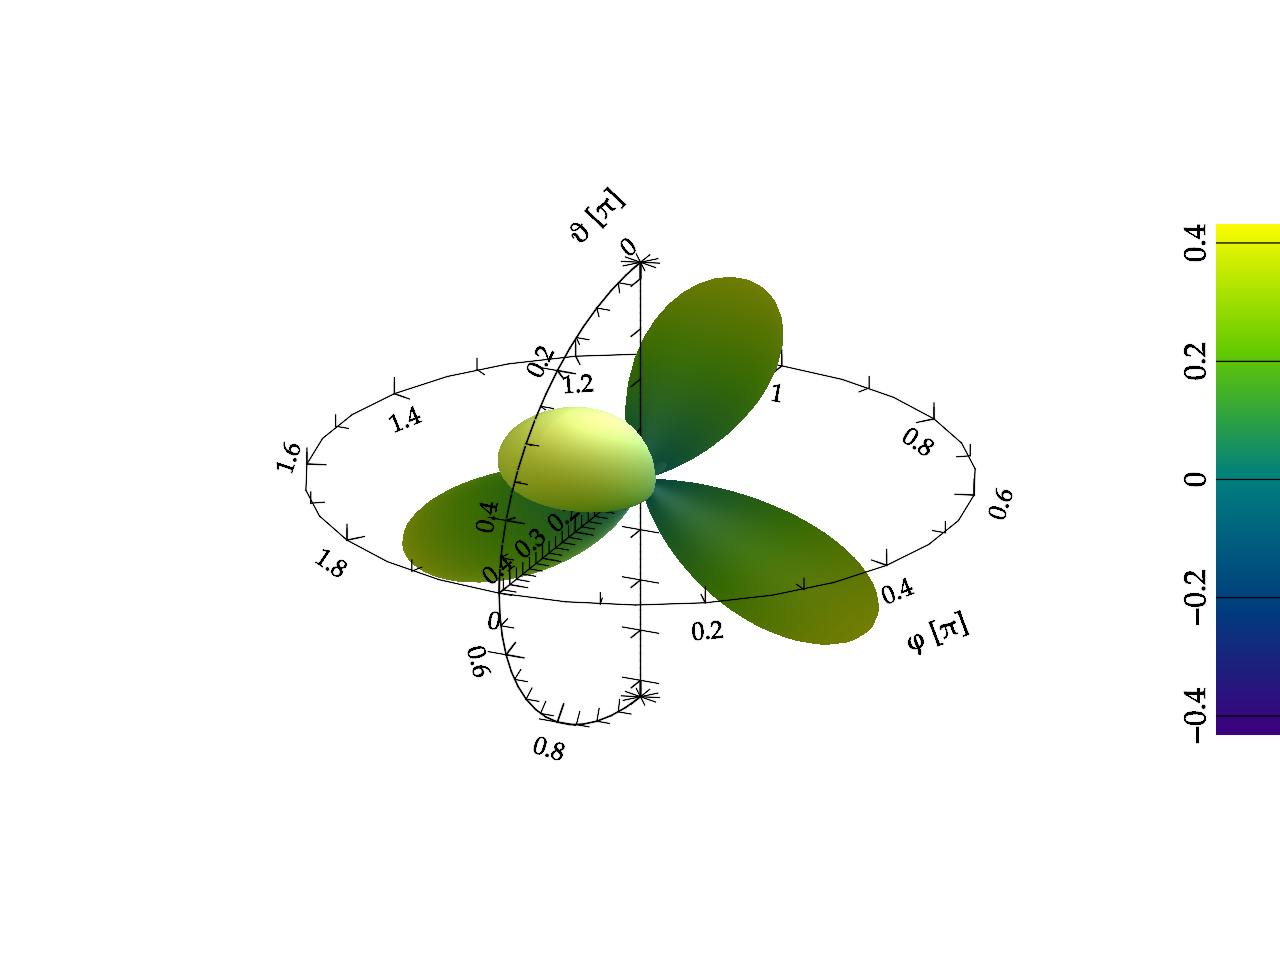
\includegraphics[width=0.45\textwidth]{_graphics/surf_1.png}}
					\caption{Ergebnisse verschiedener Koordinatensysteme}
					\label{fig:coords}
				\end{figure}
				
				Um das Koordinatensystem zu ändern, verwendet man die Option \verb+coords=KOORDINATEN+. Um beispielsweise zu polare Koordinaten zu wechseln, gibt man die folgende Zeile ein (\autoref{fig:coords}a):
				\begin{lstlisting}
plot x -set coords=polar
				\end{lstlisting}
				
				Man sieht, dass die Variable $x$ hier als $\varphi$ und der Funktionswert $y$ als radiale Koordinate $\varrho$ interpretiert werden. Die Azimuth-Achse ist in Einheiten von $\pi$ dargestellt, kann aber ggf. mittels der Option \verb+axisscale=SCALE+ geändert werden.
				
				Wenn man des Weiteren das Intervall für $x$ (ergo: $\varphi$) ändert, erhält man mit der folgende Zeile das Ergebnis von \autoref{fig:coords}b:
				\begin{lstlisting}
plot x -set coords=polar [0:10*_pi]
				\end{lstlisting}
				ggf. kann es hierbei von Vorteil sein, die Zahl der Samples mittels \verb+samples=WERT+ zu erhöhen.
				
				In Kombination mit dreidimensionalen Plotfunktionen wechselt man nun automatisch ins zylindrische System, z.B. mittels 
				\begin{lstlisting}
surf sinc(norm(y)) -set light
				\end{lstlisting}
				erhält man \autoref{fig:coords}c. Die eingebrachte Option \verb+light+ aktiviert den dreidimensionalen Lichteffekt, der das Volumen verdeutlicht.
				
				In diesem Fall wird deutlich, dass die Variable $y$ nun als $z$ und der Funktionswert $\Phi(x,y)$ nun die Funktion der radialen Variable $\varrho$ eingenommen hat.
				
				Abschließend soll hier noch das sphärische Koordinatensystem dargestellt werden. In dieses wechselt man durch z.B.
				\begin{lstlisting}
surf Y(3,2,y,x) -set coords=spherical
				\end{lstlisting}
				und erhält die nette Kugelflächenfunktion (ihr Realteil) $Y_{3\,2}(\vartheta,\varphi)$ in \autoref{fig:coords}d. In diesem Koordinatensystem hat $y$ die Funktion von $\vartheta$, $x$ ist wieder $\varphi$ und der Funktionswert $\Phi(x,y)$ wird durch die radiale Koordinate $r$ dargestellt.
				
				\helpidx{coords}
		\chapter{Tabellen: der Cache}
			Große Datensätze verwaltet \NR\ in Form von Tabellen. Die Standardtabelle für geladene Daten ist \verb+data()+, wie bereits erwähnt wurde. Allerdings ist diese \emph{Read-Only}. Als manipulierbare Tabellen in \NR\ existieren die sogenannten \emph{Caches}.
			\section{Konzept}
				Caches sind Tabellen in \NR, deren Inhalt ähnlich gewöhnlicher Variablen frei manipuliert werden kann. Ihre Größe ist beliebig und passt sich automatisch den Wünschen des Nutzers an. Standardmäßig existiert bereits der Cache \verb+cache()+, doch es können noch weitere erzeugt werden.
				
				Caches besitzen außerdem eine Autosave-Funktion. Sobald der Inhalt eines Caches verändert wird, werden diese Änderungen nach Ablauf des Autosave-Intervalls in eine externe Datei übertragen. Bei einem Neustart von \NR\ werden diese Caches und die in ihnen enthaltenen Daten automatisch wiederhergestellt und können direkt weiterverwendet werden.
			\section{Erzeugen und Entfernen von Caches}
				Um weitere Caches zu erzeugen, kann das Kommando \verb+new+ verwendet werden (dieses Kommando kann auch noch weitere Objekte generieren):\cmd{new}
				\begin{lstlisting}
new CACHE1(), CACHE2(), CACHE3(), ...
new amplitude(), phase(), results()
				\end{lstlisting}
				Die dadurch generierten Caches enthalten keine Daten und können wie \verb+cache()+ verwendet werden. Sollten ein oder mehrere Caches der Liste bereits existieren, wird \NR\ diese Caches in keinster Weise beeinflussen.
				
				\helpidx{new}
				Selbst generierte Caches können auch wieder entfernt werden, falls der Speicher nicht mehr für weitere Analysen benötigt wird:\cmd{remove}
				\begin{lstlisting}
remove CACHE1(), CACHE2(), CACHE3(), ...
remove amplitude(), phase(), results()
				\end{lstlisting}
				Der von \NR\ tatsächlich benötigte Speicher wird jedoch erst nach einem Neustart reduziert.
				
				\helpidx{remove}
				Allerdings können Caches anstatt entfernt zu werden auch umbenannt werden:\cmd{rename}
				\begin{lstlisting}
rename -CACHE1=NEUERNAME
rename -amplitude=phase
				\end{lstlisting}
				
				Um alle Caches auf einmal zu entfernen und den kompletten Speicher freizugeben, kann 
				\begin{lstlisting}
cache -clear
				\end{lstlisting}
				verwendet werden. Hierbei wird auch der tatsächlich benötigte Speicher reduziert. Für eine einfache Löschung einzelner Elemente genügt auch \cmd{delete}
				\begin{lstlisting}
delete CACHE(i1:i2,j1:j2)
				\end{lstlisting}
				
				\helpidx{cache}
			\section{Verwendung}
				Caches können verwendet werden wie die \verb+data()+-Tabelle. Ein wesentlicher Unterschied besteht jedoch in der Tatsache, dass die Inhalte von Caches auch bearbeitet werden können. Demzufolge können ihre Elemente entsprechend Variablen neue Werte zugewiesen werden:\cmd{cache()}
				\begin{lstlisting}
CACHE(:,1) = WERT1, WERT2, WERT3, ...
CACHE(4,5:) = data(:,1)
CACHE(:,1) = CACHE(2,:)
				\end{lstlisting}
				Die neuen Werte überschreiben dabei die bereits vorhandenen Werte in \verb+CACHE()+.
				
				An allen Stellen, an denen bisher \verb+data()+ verwendet wurde, können mit der identischen Syntax auch Caches eingefügt werden. Intern besteht (außer der Möglichkeit, Elemente zu ändern) kein Unterschied zwischen \verb+data()+ und den Caches:
				\begin{lstlisting}
hist cache(:,1)
stats cache()
fit cache(:,4:5) -with=A*sin(B*x+C) params=[A=1, B=1, C=0]
				\end{lstlisting}
				
				Daten, die manche Kommandos (z.B. \verb+datagrid+) erzeugen, werden teilweise automatisch in \verb+cache()+ geschrieben, teilweise erzeugen sie ihre Zielcaches auch selbst.
			\section{Sortieren, Glätten und Resamplen}
				Ggf. muss man Datenpunkte weiter modifizieren, um sie vernünftig verarbeiten zu können. \NR\ bietet hier die Möglichkeiten, die Daten zu sortieren, sie zu glätten und die Zahl der Datenpunkte zu verändern.
				
				Die Daten in einem Cache (und im Grunde auch in \verb+data()+) können auf- oder absteigend sortiert werden. Damit können z.B. bestimmte Schwellenwerte oder interessante Stellen in Messpunkten leichter gefunden werden.
				
				Mittels der Eingabe von\cmd{sort}
				\begin{lstlisting}
CACHE -sort
				\end{lstlisting}
				wird der gesamte Cache \verb+CACHE+ aufsteigend sortiert. Um ihn absteigend zu sortieren, verwendet man den Wert \verb+desc+
				\begin{lstlisting}
CACHE -sort=desc
				\end{lstlisting}
				Mittels der Option \verb+cols+ können die zu sortierenden Spalten ausgewählt werden. Außerdem können damit eine Gruppe an Spalten angegeben werden, die anhand einer Index-Spalte sortiert werden sollen (wenn beispielsweise $x$-Werte und Funktionswerte zufällig angeordnet sind, können die Funktionswerte anhand der $x$-Werte sortiert werden und die Beziehung zwischen $x$-Werten und Funktionswerten bleibt bestehen):
				\begin{lstlisting}
CACHE -sort cols=SPALTEN[SPALTENGRUPPEN]
cache -sort cols=5[2:4]
				\end{lstlisting}
				
				\helpidx{cache}
				Neben dem Sortieren der Daten können Daten im Cache von Rauschen oder anderen vergleichbaren Artefakten befreit werden. Dies erreicht man durch ein Glätten der Daten.
				
				Das Kommando\cmd{smooth}
				\begin{lstlisting}
smooth CACHE(i1:i2,j1:j2) -order=ORDNUNG
				\end{lstlisting}
				glättet den Cache \verb+CACHE+ im ausgewählten Bereich, wobei über \verb+ORDNUNG+ Punkte linear interpoliert wird. Standardmäßig wird hier zweidimensional geglättet, sofern dies aufgrund der Dimension des verwendeten Bereichs Sinn macht. Um dies auf zeilen- oder spaltenweises Glätten umzuschalten, können hier die Optionen \verb+lines+ und \verb+cols+ verwendet werden.
				
				Glätten funktioniert im Prinzip durch Einbringen eines Tiefpass-Filters. Sollten daher hochfrequente Daten interessant sein, kann Glätten diese teilweise oder auch vollständig zerstören. Als Probe bietet es sich an, die geglätteten Daten von den verrauschten Daten abzuziehen und das Ergebnis zu plotten. Wenn nur Rauschen entfernt wurde, sollte der Plot auch nur ein Rauschen zeigen.
				
				\helpidx{smooth}
				Um die Zahl der Datenpunkte anzupassen (z.B. ist die Samplerate unpassend oder man möchte zwei Datenreihen miteinander verrechnen) kann \NR\ weitere Stützstellen in die Daten interpolieren oder die Zahl der Datenpunkte ebenso auch verringern.
				
				Dies wird mittels\cmd{resample}
				\begin{lstlisting}
resample CACHE(i1:i2,j1:j2) -samples=SAMPLES
				\end{lstlisting}
				erreicht. Im gewählten Bereich wird dabei spaltenweise die Zahl der Stützstellen zu \verb+SAMPLES+ verändert. Sollte \verb+SAMPLES+ größer als der gewählte Bereich sein, geht keine Information verloren, da die neuen Datenpunkte aus den bisherigen interpoliert werden. Wird Zahl hingegen kleiner gewählt, muss Information verloren gehen..
				
				\helpidx{resample}
			\section{Statistik-Funktionalität}
				Caches (und auch die \verb+data()+-Tabelle) können zusätzlich zu \verb+stats+ und den Statistik-Funktionen (\verb+std()+, \verb+avg()+, \ldots) auch globale Statistikoperationen ausführen. Dazu werden die Caches als Kommando verwendet und mit den Statistikfunktionen als Parameter ausgeführt (in diesem Fall tauchen keine Klammern in dem Ausdruck auf):
				\begin{lstlisting}
CACHE -avg
CACHE -std
...
				\end{lstlisting}
				Dies berechnet Mittelwert/Standardabweichung/etc. der gesamten Tabelle als gemeinsamen Wert. Mit zusätzlichen Optionen kann dies noch weiter eingeschränkt werden: die Option \verb+grid+ berechnet die entsprechenden Statistikwerte, wobei der Cache als Datengitter interpretiert wird. Die Option \verb+cols+ berechnet die Werte spalten- und \verb+lines+ zeilenweise. Die Optionen \verb+lines+ und \verb+cols+ können mit \verb+grid+ kombiniert werden.
		\chapter{NumeRe-Scripte}
			\NR-Scripte bieten die Möglichkeit, komplexe Rechnungen und häufig wiederkehrende Analysen in eine Datei auszulagern, von der sie einfach und wiederholt ausgeführt werden können.
			\section{Konzept}
				Das Konzept hinter \NR-Scripten ist simpel: alle Eingaben in die \NR-Konsole werden zeilenweise in eine Textdatei geschrieben, die im Anschluss von \NR\ gelesen wird. \NR\ wird dann die Ausdrücke und Kommandos in der entsprechenden Reihenfolge abarbeiten und auswerten.
				
				Der Vorteil liegt auf der Hand: die Befehlskette kann einfach wiederholt werden und Fehler können schnell und simpel korrigiert werden. Außerdem kann in Notepad++ die Syntaxhighlighting für \NR\ geladen werden.
				\paragraph{Anmerkung}
					In einem späteren Kapitel werden auch \NR-Prozeduren besprochen. Diese repräsentieren die Programmierbarkeit von \NR. Die meisten Problemstellungen, die keine allzu komplexen Abstraktionen erfordern, lassen sich aber problemlos mithilfe von \NR-Scripten lösen.
				
				\helpidx{script}
			\section{Syntaxhighlighting}
				Um die Syntaxhighlighting verwenden zu können, wird \href{https://notepad-plus-plus.org/}{Notepad++} benötigt. Dieser Editor muss gestartet werden, dann im Menü ">Sprachen"< der Punkt ">Eigene Sprache definieren \ldots"< gewählt werden. Im sich daraufhin öffnenden Fenster wählt man ">Importieren"< und navigiert zum \NR-Stammverzeichnis. Hier sollten die zwei Dateien ">numere\_nprc\_highlighting.xml"< und ">numere\_nscr\_highlighting.xml"< zu finden sein. Man wähle eine, klicke auf ">Öffnen"< und wiederhole den Schritt für die zweite Datei.
				\begin{figure}[p]%
					\centering
					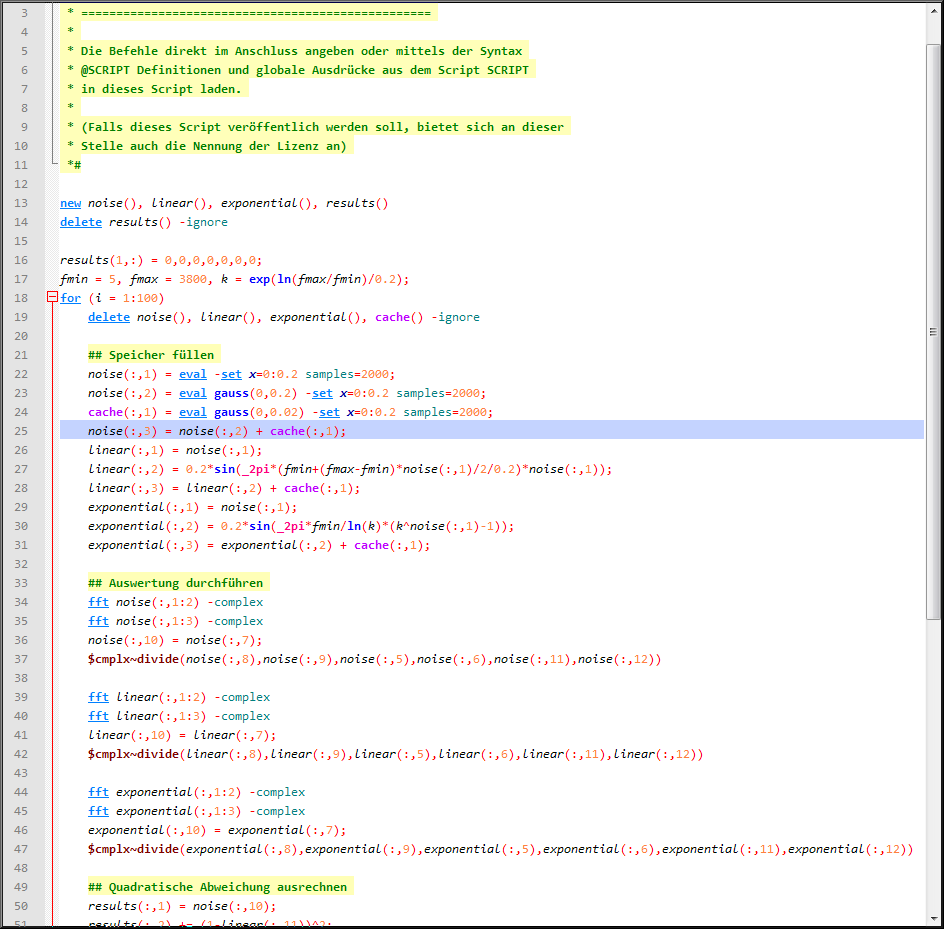
\includegraphics[width=\textwidth]{_graphics/highlighting.png}
					\caption{Ein Beispiel der \NR-Syntaxhighlighting}
					\label{fig:highlighting}
				\end{figure}
				
				Nun wird Notepad++, sobald eine *.nscr- oder *.nprc-Datei geöffnet wird, die entsprechende Syntaxhighlighting laden (\autoref{fig:highlighting}). Durch die farbliche Hervorhebung der verschiedenen Syntaxelemente sollten \NR-Scripte einfach und fehlerfrei zu schreiben sein. Außerdem bietet Notepad++ mit der Klammerhervorhebung eine direkte Möglichkeit, die verwendeten Klammern zu prüfen.
				
				Es steht jedem frei, die Farbgebung der Syntaxhighlighting zu bearbeiten und eine eigene zu wählen. Dies kann man ebenfalls unter ">Eigene Sprache definieren \ldots"< durchführen. Man wähle im Dropdown-Menü den Eintrag ">NumeRe-Script"< und verwende die ">Stil"<-Schaltflächen, die in den entsprechenden Tabs auftreten, um Farbgebung und Schrifterscheinungsbild zu beeinflussen. Um den ursprünglichen Zustand wiederherzustellen, kann die Datei erneut importiert werden.
			\section{Ein einfaches Script}
				Da ein kompliziertes Script, wie es in \autoref{fig:highlighting} zu sehen ist, sicher zu komplex für den ersten Versuch ist, soll hier ein viel einfacheres Beispiel gezeigt werden.
				
				Um ein \NR-Script schnell und einfach zu erstellen, gebe man 
				\begin{lstlisting}
new -script=erstes
				\end{lstlisting}
				in die \NR-Konsole ein. Es wird ein \NR-Script ">erstes.nscr"< in \verb+<scriptpath>+ erzeugt. Die Zeile\cmd{edit}
				\begin{lstlisting}
edit erstes.nscr
				\end{lstlisting}
				öffnet dieses \NR-Script im verknüpften Texteditor, so dass es bearbeitet werden kann. (Die Dateierweitung ist hier nötig, da \verb+edit+ sonst nicht im korrekten Verzeichnis nach dem Script sucht) Zwischen die beiden im Script erscheinenden Textblöcke (Alles zwischen \verb+#*...*#+ ist ein Kommentar und wird von \NR\ nicht interpretiert) füge man die folgenden Zeilen ein:
				\begin{lstlisting}
#* Cacheinhalt komplett loeschen *#
delete cache() -ignore

#* Zufallszahlen erzeugen *#
random -lines=1e5 cols=2 distrib=uniform mean=0.5 width=1

#* Innerhalb des Viertel-Einheitskreises? *#
cache(:,3) = (cache(:,1)^2+cache(:,2)^2) <= 1 ? true : false;

#* PI berechnen *#
4*sum(cache(:,3))/1e5
				\end{lstlisting}
				wobei \verb+##+ einen Zeilenkommentar einleitet, der von \NR\ ebenfalls ignoriert wird. Das \verb+ignore+ in der zweiten Zeile unterdrückt die Sicherheitsabfrage, ob der Cacheinhalt wirklich gelöscht werden soll. \cmd{random}\verb+random+ erzeugt Zufallszahlen und schreibt selbige in den Cache. Hier werden zweimal 100\,000 gleichverteilte Zufallszahlen im Intervall $[0;1]$ erzeugt.
				
				Die dritte Anweisung ist die tückischste. Hier wird an die dritte Spalte in \verb+cache()+ das Ergebnis einer Bedingung zugewiesen. Sinngemäß steht hier so was wie
				\begin{quotation}
					\noindent\emph{">Ist der Vektorbetrag kleiner-gleich als 1, dann schreibe ">wahr"<, sonst schreibe ">falsch"< in den Cache."<}
				\end{quotation}
				Der sogenannte \emph{Ternary}-Operator
				\begin{lstlisting}
BEDINGUNG ? DANN_WERT : SONST_WERT
				\end{lstlisting}\cmd{()? \ldots\ : \ldots}
				ist eine Abkürzung für die \verb+if...else...endif+-Verzweigung, die an späterer Stelle besprochen werden soll. Der Vorteil des \emph{Ternarys} ist, dass er tendenziell schneller ausgeführt wird, dafür jedoch keine Kommandos aufnehmen kann. Eine Auflistung aller Logikausdrücke erhält man durch
				\begin{lstlisting}
list -logic
				\end{lstlisting}
				Am Ende der Zeile findet man auch ein Semikolon \verb+;+. Dieses unterdrückt die Ausgabe der Ergebnisse auf der \NR-Konsole.
				
				Das gesamte \NR-Script ist eine ganz simple \emph{Monte-Carlo}-Simulation. Es werden zufällig Punkte auf einem Quadrat mit der Kantenlänge 1 platziert und anschließend gezählt, wie viele der Punkte auf dem (Viertel-)Einheitskreis liegen, der Teil des Quadrates ist. Unter der Annahme, dass die Wahrscheinlichkeit für jeden Punkt im Quadrat gleich hoch ist, muss das Verhältnis von den im Kreis liegenden zur Gesamtzahl der Punkte $\pi/4$ sein.
				
				Führt man das \NR-Script mittels\cmd{start}
				\begin{lstlisting}
start erstes
				\end{lstlisting}
				aus (\verb+random+ benötigt einen Moment), so bekommt man Ergebnisse ähnlich zu
				\begin{lstlisting}
3.1364
3.13668
3.1454
3.13952
...
				\end{lstlisting}
				Diese Zahlen liegen schon relativ nahe an $\pi$ dran, obwohl sie im Grunde nur durch eine clevere Ausnutzung des Zufalls generiert wurden.
				
				Erhöht man die Zahl der erzeugten Zufallszahlen (z.B. \verb+1e6+ statt \verb+1e5+), so wird die Annäherung zunehmend genau. Allerdings unterstützt der Cache nicht beliebig viele Elemente. Für noch größere Zahlen muss man also auf andere Verfahren zurückgreifen.
	\part{Fortgeschrittene Bedienung}
		\chapter{Eigene Funktionen}
			\NR\ bringt bereits eine große Zahl vordefinierter Funktionen mit (siehe \verb+list -func+). Dennoch kann es häufig hilfreich und praktisch sein, wenn man sich eigene Funktionen definieren kann, die z.B. bereits bestehende zusammenfassen. \NR\ kann bis zu 100 selbst definierte Funktionen speichern.
			\section{Definition}
				\cmd{define}Eine eigene Funktion wird mittels
				\begin{lstlisting}
define meine_funktion(ARGS) := AUSDRUCK(ARGS)
				\end{lstlisting}
				definiert. Diese Zeile erzeugt die Funktion \verb+meine_funktion()+, die den komplexeren Ausdruck der Argumente zusammenfasst. Die Bezeichnungen und die Zahl der Argumente können beliebig gewählt werden, so lange sie die Maximalzahl von 10 nicht überschreiten. Wenn das letzte Argument der Funktion ">\verb+...+"< lautet, so kann für dieses Argument von einem bis zu beliebig vielen Werten angegeben werden. Der definierte Ausdruck muss dann allerdings auch mit beliebig vielen Werten umgehen können, z.B.:
				\begin{lstlisting}
define meine_funktion(x,...) := x*sum(...)
				\end{lstlisting}
				
				Der Name der Funktion ist auch beliebig, so lange er nicht mit einer Ziffer beginnt oder einer bereits (vor-)definierten Funktion entspricht.
				
				\cmd{redefine}Mit
				\begin{lstlisting}
redefine meine_funktion(ARGS) := NEUER_AUSDRUCK(ARGS)
				\end{lstlisting}
				kann die Funktion \verb+meine_funktion()+ umdefiniert werden. Hierbei müssen die neuen Argumente natürlich nicht mit den bisherigen übereinstimmen.
				
				Selbst definierte Funktionen können mit Kommentaren versehen werden, um zu erläutern, was der Zweck der Funktion ist. Dieser Kommentar wird dann unter
				\begin{lstlisting}
list -define
				\end{lstlisting}
				zusammen mit der Definition angezeigt.
				
				Der Kommentar kann bei der Definition mittels
				\begin{lstlisting}
define meine_funktion(ARGS) := AUSDRUCK(ARGS) -set comment="KOMMENTAR"
				\end{lstlisting}
				angegeben werden. Eine nachträgliche Kommentierung kann mittels \verb+redefine+ durchgeführt werden.
				
				\helpidx{define}
				\cmd{undefine}Um selbst definierte Funktionen wieder zu entfernen, verwendet man
				\begin{lstlisting}
undefine meine_funktion()
				\end{lstlisting}
				am Programmende wird der Funktionsspeicher jedoch auch automatisch geleert. Möchte man dies verhindern, kann man entweder
				\begin{lstlisting}
define -save
				\end{lstlisting}
				eingeben und beim nächsten Start
				\begin{lstlisting}
define -load
				\end{lstlisting}
				um die Funktionen zu laden, oder man aktiviert die automatische Definitionsverwaltung durch
				\begin{lstlisting}
set -defcontrol=true
				\end{lstlisting}
				
				\helpidx{set}
			\section{Bedingte Definition}
				In \NR-Scripten kann es von Vorteil sein, wenn \NR\ nicht bei jedem Durchlauf den Fehler bringt, dass eine Funktion, die im Script definiert werden soll, bereits definiert ist. Für diesen Fall gibt es die Möglichkeit, entweder \verb+redefine+ zu verwenden, oder man gibt stattdessen\cmd{ifndefined}
				\begin{lstlisting}
ifndefined meine_funktion(ARGS) := ...
				\end{lstlisting}
				an. Nun wird die Funktion nur dann definiert, wenn sie nicht schon bereits im Funktionsspeicher vorhanden ist.
			\section{Verwendung}
				Eine selbst definierte Funktion kann wie die vordefinierten Funktionen verwendet werden, da sie intern vor der eigentlichen Auswertung in ihre Definition umgewandelt werden. Daher ergeben
				\begin{lstlisting}
meine_funktion(1,2,3)
				\end{lstlisting}
				und 
				\begin{lstlisting}
sin(1)+cos(2)+sinc(3)
				\end{lstlisting}
				für die Definition
				\begin{lstlisting}
define meine_funktion(x,y,z) := sin(x)+cos(y)+sinc(z)
				\end{lstlisting}
				dasselbe Ergebnis. Es können auch weniger Werte angegeben werden, wie die definierte Funktion Argumente besitzt. \NR\ wird die fehlenden Werte dann durch \verb+0+ ergänzen.
		\chapter{Zeichenketten}
			Neben numerischen Werten kann \NR\ auch mit Zeichenketten umgehen. Zunächst eingeführt, um die Spaltentitel der Tabellen formatieren zu können, sind die Zeichenkettenfunktionen inzwischen aber zu einem festen und sicher verwendbaren Konstrukt in \NR's Architektur geworden.
			\section{Konzept}
				Zeichenketten sind zunächst aneinandergereihte Zeichen, die \NR\ nicht als Variablen oder numerische Werte interpretiert. Um dies zu erreichen, sind Zeichenketten durch umschließende Anführungszeichen einzugeben:\cmd{"\ldots"\:}
				\begin{lstlisting}
"Dies ist eine Zeichenkette."
				\end{lstlisting}
				Der eigentliche Inhalt der Zeichenkette sind alle Zeichen zwischen den Anführungszeichen. Die Zeichenkette \verb+""+ ist folglich leer und hat die Länge 0.
				
				Zeichenketten können durch spezielle Funktionen modifiziert werden: es gibt Funktionen zur Umwandlung von Groß- in Kleinbuchstaben (oder umgekehrt), zum Suchen von Zeichenketten in Zeichenketten, zum Extrahieren einer Zeichenkette aus einer anderen, zum Ersetzen von Zeichenketten in einer anderen, usw. Der eigentliche Vorteil von Zeichenketten sind die Möglichkeit, Ausgaben zu formatieren und das Verarbeiten mehrerer Dateien zu automatisieren. (Außerdem sind sie Grundvoraussetzung für die Programmierung durch \NR-Prozeduren)
				
				\helpidx{string}
			\section{Variablentyp}
				Neben den numerischen Variablen und den Tabellen sind die Zeichenkettenvariablen (auch \emph{strings}) der dritte Variablentyp in \NR. Numerische Variablen können jedoch nicht in Zeichenketten und Zeichenkettenvariablen nicht in numerische umgewandelt werden. Ihre jeweiligen Inhalte jedoch schon (s.u.).
				
				\NR\ erkennt neue Zeichenkettenvariablen automatisch anhand der Deklaration. Diese muss -- im Gegensatz zur Deklaration numerischer Variablen, welche \emph{on-the-fly} vonstatten gehen kann -- \emph{immer} mit einem Wert in Form einer Zeichenkette erfolgen (zumindest einer leeren Zeichenkette):
				\begin{lstlisting}
numerische_variable = 3.1415926
auch_numerisch
zeichenkette = "Hallo Welt!"
auch_zeichenkette = ""
				\end{lstlisting}
				Eine Deklaration mit dem Rückgabewert einer Zeichenkettenfunktion ist natürlich ebenfalls möglich.
				
				Neben den Zeichenkettenvariablen kennt \NR\ noch das \cmd{string()}\verb+string()+-Objekt. Dies ist im Prinzip eine einspaltige Tabelle, die beliebig viele Zeichenketten aufnehmen kann. In den Argumentklammern kann die Bereichssyntax verwendet werden, um einen Satz an Zeichenketten zu extrahieren, oder ein einzelner Index für eine einzelne Zeichenkette. Bleiben hier die Argumentklammern leer, wird automatisch die zuletzt zugewiesene Zeichenkette verwendet.
				
				\helpidx{string}
				Mithilfe von Zeichenketten können auch die Tabellenköpfe von \verb+data()+ und den Caches geändert werden. Dies erreicht man durch\cmd{data(\#,:)\\cache(\#,:)}
				\begin{lstlisting}
data(#,1) = "Spaltenueberschrift 1"
cache(#,:) = "Spalte 1", "Spalte 2", "Spalte 3"
				\end{lstlisting}
				Wie man sieht, ist auch hier die Bereichssyntax möglich. Die Raute \verb+#+ referenziert die Tabellenköpfe.
				
				\helpidx{cache}
			\section{Konvertierung}
				Der Wert einer Zeichenkettenvariable kann zu einem numerischen umgewandelt werden und umgekehrt. Dabei wird der Inhalt der Zeichenkette ggf. als neue Variable, als Ausdruck oder ggf. sogar als Kommando interpretiert. Hierbei gibt es zwei Funktionen:
				\begin{lstlisting}
to_value()
to_cmd()
				\end{lstlisting}
				Die Funktion \verb+to_value()+ wandelt die übergebene Zeichenkette in einen ma\-the\-ma\-tisch-nu\-me\-ri\-schen Ausdruck um und wertet ihn entsprechend aus. \verb+to_cmd()+ wandelt die Zeichenkette hingegen in einen Kommandoausdruck um.
				
				Die Umkehrung kann auf verschiedene Arten vonstatten gehen:\cmd{\#VAR\\\#(EXPRESSION)}
				\begin{lstlisting}
#VAR
#(EXPRESSION)
valtostr(EXPR,C,N)
to_string()
string_cast()
				\end{lstlisting}
				Die Syntax \verb+#VAR+ oder \verb+#(EXPRESSION)+ wertet den darauffolgenden Ausdruck/Variable aus und wandelt den numerischen Wert direkt in eine Zeichenkette um. Zwischen \verb+#+ und dem Ausdruck können noch ein oder mehrere \verb+~+ eingefügt werden, welche die Zeichenzahl durch vorangestellte \verb+0+ auf eine entsprechende Zahl an Zeichen zzgl. des \verb+#+'s ergänzen. Dies wird durch die Funktion \verb+valtostr()+ verallgemeinert, die das Füllzeichen mittels des Zeichens \verb+C+ übergeben bekommt. Die Funktion \verb+to_string()+ wandelt alles, was keine Zeichenkette ist, direkt in eine Zeichenkette um, ohne etwas zuvor auszuwerten, und \verb+string_cast()+ wandelt selbst Zeichenkettenvariablennamen in Zeichenketten um.
		\chapter{Schleifen und Verzweigungen}
			Der Ablauf von \NR-Scripten (und den im nächsten Kapitel eingeführten \NR-Pro\-ze\-du\-ren) kann durch die Einführung von Schleifen und Verzweigungen teils drastisch vereinfacht werden (was nicht heißen soll, dass Schleifen und Verzweigungen nicht auch direkt in der \NR-Konsole verwendbar wären).
			\section{Verzweigungen}
				Eine Verzweigung ist eine Stelle im Script, an der der weitere Verlauf des Scriptes von einer gegebenen Bedingung abhängt. Solche Verzweigungen werden durch das folgende Konstrukt repräsentiert:\cmd{if ()\\\ldots\\elseif ()\\\ldots\\else\\\ldots\\endif}
				\begin{lstlisting}
if (BEDINGUNG1)
	AUSFUEHREN, FALLS WAHR
elseif (BEDINGUNG2)
	AUSFUEHREN, FALLS BEDINGUNG1 FALSCH UND BEDINGUNG2 WAHR
else
	AUSFUEHREN, FALLS ALLE BEDINGUNGEN FALSCH
endif
				\end{lstlisting}
				
				Eine Verzweigung muss mindestens aus einem \verb+if ()+ und einem abschließenden \verb+endif+ bestehen. Es können dazwischen beliebig viele \verb+elseif ()+ und höchstens ein \verb+else+ als allgemeiner \emph{Sonst-Fall} verwendet werden, wobei \verb+else+ als letzter Fall vor \verb+endif+ verwendet werden muss. Eine Verzweigung, die nur aus einem \verb+if ()+ und einem \verb+endif+ besteht, wird nur dann ausgeführt, wenn die Bedingung erfüllt ist, anderenfalls wird sie komplett übersprungen.
				
				Die Blöcke, die zwischen \verb+if ()+, \verb+endif+ und den restlichen Schlüsselwörtern stehen, können beliebig lange sein und sowohl Ausdrücke als auch Kommandos enthalten. Zusätzlich können die Blöcke auch weitere Verzweigungen und Schleifen enthalten.
				
				\helpidx{if}
			\section{Bedingte Schleifen}
				\cmd{while ()\\\ldots\\endwhile}Eine bedingte Schleife wird nur (so lange) ausgeführt, so lange die Bedingung wahr ist. Die Syntax dazu ist
				\begin{lstlisting}
while (BEDINGUNG)
	AUSFUEHREN, SO LANGE WAHR
endwhile
				\end{lstlisting}
				Auch hier können Ausdrücke und/oder Kommandos im Ausführungsblock enthalten sein, ebenso wie weitere Verzweigungen und Schleifen.
				
				\helpidx{while}
			\section{Zählschleifen}
				Eine Zählschleife macht ihre Auswertung vom Wert einer Indexvariable abhängig. Über den Bereichssyntax muss hierbei der Start- und Endwert vorgegeben werden. Sollte der Endwert \emph{kleiner} als der Startwert sein, zählt die Zählschleife automatisch rückwärts. Nach jedem Schleifendurchlauf wird der Indexwert automatisch um eins erhöht (bzw. erniedrigt, wenn die Schleife rückwärts zählt). Der Index selbst kann in der Schleife als Variable verwendet werden.
				
				Die Syntax einer Zählschleife lautet wie folgt:
				\cmd{for ()\\\ldots\\endfor}\begin{lstlisting}
for (INDEX = START:END)
	AUSFUEHREN, SO LANGE INDEX IN [START;END]
endfor
				\end{lstlisting}
				Ebenso wie zuvor können in diesem Block weitere Ausdrücke, Kommandos, Schleifen und Verzweigungen verwendet werden. Die Indexvariable wird nach Abschluss der Schleife -- falls sie nicht bereits vor der Schleife bekannt war -- automatisch gelöscht.
				
				\helpidx{for}
			\section{Ablaufkontrollen}
				Auf den Ablauf einer Schleife kann mit einem der beiden Kommandos\cmd{continue\\break}
				\begin{lstlisting}
continue
break
				\end{lstlisting}
				weiter Einfluss genommen werden. \verb+continue+ überspringt den restlichen Schleifenablauf und beginnt sofort einen neuen Schleifendurchlauf. Hingegen bricht \verb+break+ die gesamte Schleife sofort ab und springt in die nächsthöhere (also umschließende) Schleife, sofern vorhanden. Falls es keine umschließende Schleife gibt, wird \NR\ mit dem restlichen Script-/Programmablauf fortfahren. Eine sinnvolle Anwendung dieser Kommandos kann eigentlich nur aus einer \verb+if+-Ver\-zwei\-gung im inneren der betreffenden Schleife geschehen.
				
				\helpidx{if}
		\chapter{Matrix-Operationen}
			\NR\ ist in Form einer Tabellenkalkulation ausgelegt, da es in der Wissenschaft ungemein wahrscheinlicher ist, dass Messreihen verarbeitet werden müssen, als dass eine Matrix-Operation durchgeführt werden muss. Dennoch ist auch \NR\ in der Lage, mit Matrizen umzugehen und wesentliche Auswertungen durchzuführen.
			\section{Ausführen einer Matrix-Operation}
				Matrix-Operationen verbergen sich hinter dem \verb+matop+- bzw. \verb+mtrxop+-Kommando (Synonyme)\cmd{matop}. Dieses Kommando leitet einen Ausdruck ein, der mittels Matrix-Operationen verarbeitet werden soll, wobei die Matrizen durch Ausschnitte des Caches, eines Datenfiles oder durch spezielle Funktionen repräsentiert werden. Hierbei ist jedoch noch zu beachten, dass alle Auswertungen (also auch die Multiplikation zweier Matrizen) standardmäßig elementweise durchgeführt werden.
				\begin{lstlisting}
matop CACHE(i1:i2,j1:j2) * DATA(i1:i2,j1:j2) + CACHE(:,:) / ...
				\end{lstlisting}
				
				Um eine Matrix-Matrix- oder Matrix-Vektor-Multiplikation durchzuführen, muss der \cmd{... ** ...}\verb+**+-O\-pe\-ra\-tor verwendet werden. Dieser Operator hat eine höhere Priorität als alle anderen Operatoren, daher ist es ggf. wichtig, entsprechend zu klammern. Außerdem ist es wichtig, dass die Dimensionen der Matrizen gemäß den Regeln der Matrizenmultiplikation übereinstimmen.
				\begin{lstlisting}
matop CACHE() ** (DATA() * CACHE())
				\end{lstlisting}
				
				Wenn \verb+matop+ kein Zielcache, in den die Matrix gespeichert werden kann, vorgegeben wird, wird automatisch \verb+matrix()+ verwendet. In diesem Fall werden die Inhalte von \verb+matrix()+ komplett überschrieben.
				
				\helpidx{matop}
			\section{Spezielle Funktionen}
				Spezielle oder temporäre Matrizen bzw. weitergehende Matrix-Operationen können mit den folgenden Funktionen erreicht werden, wenn sie innerhalb des \verb+matop+-Kommandos verwendet werden.
				\begin{itemize}
					\item \verb+cross(MAT)+ berechnet das $n$-dimensionale Kreuzprodukt der $n\times(n-1)$-Matrix \verb+MAT+.
					\item \verb+det(MAT)+ berechnet die Determinante der quadratischen Matrix \verb+MAT+.
					\item \verb+diag(x,y,z,...)+ erzeugt eine Diagonalmatrix mit \verb+x,y,z,...+ auf der Hauptdiagonalen.
					\item \verb+diagonalize(MAT)+ diagonalisiert die quadratische Matrix \verb+MAT+. Sollten die berechneten Diagonalelemente komplex sein, wird eine $n\times2\,n$-Matrix zurückgegeben mit den Realteilen auf der unteren und den Imaginärteilen auf der oberen ersten Nebendiagonalen.
					\item \verb+eigenvals(MAT)+ berechnet die Eigenwerte der quadratischen Matrix MAT und gibt diese in Form eines Vektors zurück. Sind die Eigenwerte komplex, werden sie als zweispaltige Matrix zurückgegeben, mit dem Realteil in der ersten und dem Imaginärteil in der zweiten Spalte.
					\item \verb+eigenvects(MAT)+ berechnet die Eigenvektoren der quadratischen Matrix MAT und gibt diese in Form einer Matrix mit den Eigenvektoren als Spalten zurück. Sind die Eigenvektoren komplex, werden sie als $n \times 2\,n$-Matrix zurückgegeben, mit den Realteilen in den ungeraden und den Imaginärteilen der Vektorkomponenten in den geraden Spalten.
					\item \verb+identity(n)+ generiert eine $n\times n$-Einheitsmatrix
					\item \verb+invert(MAT)+ invertiert die symmetrische Matrix \verb+MAT+, falls eine Inverse existiert.
					\item \verb+matfc(X,Y,Z,...)+ konstruiert eine Matrix aus den Spalten \verb+X,Y,Z,...+. Fehlende Elemente werden durch 0 ergänzt.
					\item \verb+matfcf(X,Y,Z,...)+ konstruiert eine Matrix aus den Spalten \verb+X,Y,Z,...+. Fehlende Elemente werden aus den vorhandenen logisch ergänzt.
					\item \verb+matfl(X,Y,Z,...)+ konstruiert eine Matrix aus den Zeilen \verb+X,Y,Z,...+. Fehlende Elemente werden durch 0 ergänzt.
					\item \verb+matflf(X,Y,Z,...)+ konstruiert eine Matrix aus den Zeilen \verb+X,Y,Z,...+. Fehlende Elemente werden aus den vorhandenen logisch ergänzt.
					\item \verb+one(n,m)+ erzeugt eine $n\times m$-Matrix, die vollständig mit 1-en gefüllt ist. Wird nur eine Dimension vorgegeben, erzeugt \NR\ eine symmetrische Matrix.
					\item \verb+solve(MAT)+ löst das lineare Gleichungssystem, das durch die Matrix \verb+MAT+ beschrieben wird.
					\item \verb+trace(MAT)+ berechnet die Spur der quadratischen Matrix \verb+MAT+.
					\item \verb+transpose(MAT)+ transponiert die Matrix \verb+MAT+ (vertauscht Zeilen mit Spalten).
					\item \verb+zero(n,m)+ erzeugt eine $n\times m$-Matrix, die vollständig mit 0-en gefüllt ist. Wird nur eine Dimension vorgegeben, erzeugt \NR\ eine symmetrische Matrix.
				\end{itemize}
				\begin{lstlisting}
matop matfc({1,2,3},{4,5,6},{7,8,9})
/ 1  4  7 \
| 2  5  8 |
\ 3  6  9 /
matop zero(2,4)
/ 0  0  0  0 \
\ 0  0  0  0 /
				\end{lstlisting}
		\chapter{Spezielle Kommandos}
			An dieser Stelle sollen einige spezielle Kommandos Erwähnung finden, die bisher noch nicht genannt wurden, aber einen großen Teil von \NR's Funktionalität ausmachen.
			\section{Nullstellen}
				\NR\ kann mittels des Kommandos \verb+zeroes+\cmd{zeroes} Nullstellen von Funktionen und Datenreihen suchen. Im Falle von Datenreihen gibt dieses die Indices der Nullstellen (bzw. des Punktes, der sich am nächsten befindet) oder, wenn ein $x$-Datensatz übergeben wurde, den entsprechenden $x$-Wert zurück:
				\begin{lstlisting}
zeroes DATEN()
zeroes DATEN() -set x=XWERTE()
				\end{lstlisting}
				
				Wenn die Nullstellen von Funktionen bzw. der Schnittpunkt zweier Funktionen gesucht werden soll, muss allerdings ein $x$-Intervall vorgegeben werden, in dem \NR\ suchen soll:
				\begin{lstlisting}
zeroes f(x) -set x=x1:x2
				\end{lstlisting}
				
				Im entsprechenden Hilfeartikel finden sich noch weitere Optionen, die \verb+zeroes+ übergeben werden können.
				
				\helpidx{zeroes}
			\section{Extrema}
				Ähnlich wie bei \verb+zeroes+ verhält es sich bei \verb+extrema+.\cmd{extrema} \NR\ kann die Extrema von Funktionen und Datensätzen bestimmen. Bei Funktionen werden die $x$-Werte zurückgegeben, bei Datensätzen die Indices bzw. die $x$-Werte der Punkte, die das Extrema beschreiben.
				\begin{lstlisting}
extrema f(x) -set x=x1:x2
extrema DATEN()
extrema DATEN() -set x=XWERTE()
				\end{lstlisting}
				\paragraph{Anmerkung}Im Gegensatz zu Nullstellen sind Extrema von Datensätzen nicht \emph{wirklich eindeutig} bestimmbar -- zumindest, wenn die Daten mit Rauschen behaftet sind. Dies ist aber in den meisten Fällen erfüllt, daher beschränkt \NR\ sich immer auf die Bestimmung der Indices bzw. $x$-Werte der Maxima bzw. Minima eines Datensatzes anstatt sie, wie bei \verb+zeroes+ ggf. zu interpolieren. Ebenso kann \NR\ aufgrund der numerischen Berechnung Sattelpunkte gar nicht oder nur sehr schlecht identifizieren, da diese Stellen keine Vorzeichenwechsel in der Ableitung aufweisen.
				
				\helpidx{extrema}
			\section{Integration}
				\NR\ kann sowohl Funktionen als auch Daten mittels \verb+integrate+\cmd{integrate} numerisch integrieren, wobei nur für Funktionen eine 2D-Integration unterstützt wird. Ob eine 2D-Integration ausgeführt werden soll, entscheidet \NR\ anhand der übergebenen Integrationsintervalle. Wenn nur ein $x$-Intervall übergeben wird, wird eine 1D-Integration ausgeführt; wenn zusätzlich ein $y$-Intervall übergeben wird, wird zweidimensional integriert.
				
				Mittels des Parameters \verb+-set+ werden das Integrationsintervall und weitere Optionen übergeben, wie z.B. die Präzision der Integration, die Methode, ob die Funktionswerte des Integrals zurückgegeben werden sollen, etc. Details finden sich im entsprechenden Hilfeartikel.
				\begin{lstlisting}
integrate x^2 -set [1:2]
				\end{lstlisting}
				
				Um 1D-Datensätze zu integrieren, sind diese statt der Funktion zu übergeben: wenn nur eine Spalte übergeben wird, wird nur die Summe des Datensatzes berechnet, werden zwei Spalten angegeben, wird die erste als $x$- und die zweite als die entsprechenden $y$-Werte interpretiert und das entsprechende Integral bestimmt.
				\begin{lstlisting}
integrate DATEN(:,1)
integrate DATEN(:,1:3)
				\end{lstlisting}
				
				\helpidx{integrate}
			\section{Ableitung}
				Neben der Integration ist \NR\ auch zur numerischen Ableitung erster Ordnung mittels des Kommandos \verb+diff+\cmd{diff} fähig. Abhängig von den übergebenen Parametern wird dabei die Ableitung an der vorgegebenen $x$-Stelle oder entsprechend der Zahl der gewünschten Stützstellen (\verb+samples+) über ein ganzes Intervall berechnet.
				\begin{lstlisting}
diff sin(x) -set x=1
diff sin(x) -set [0:1]
				\end{lstlisting}
				
				Ebenfalls ist \NR\ in der Lage, Datensätze numerisch zu differenzieren. Wenn hierbei eine Spalte übergeben wird, wird der Abstand zwischen den Stützstellen als 1 angenommen, wenn zwei Spalten angegeben werden, wird die erste als $x$- und die zweite als $y$-Werte interpretiert.
				\begin{lstlisting}
diff DATEN(:,1)
diff DATEN(:,1:2)
				\end{lstlisting}
				Hierbei werden nur die $y$-Werte der Ableitung berechnet. Mittels der Option \verb+xvals+ werden stattdessen die neuen $x$-Werte (die mit den vorgegeben nicht übereinstimmen) bestimmt und zurückgegeben.
				
				\helpidx{diff}
			\section{Taylorentwicklung}
				\NR\ kann mittels \verb+taylor+\cmd{taylor} Funktionen in Abhängigkeit von einer Variablen mittels des Taylor-Verfahrens durch ein Polynom der Ordnung $n \geq 0$ approximieren. Dieses Polynom muss allerdings (außer an der Entwicklungsstelle) nirgends mit der approximierten Funktion übereinstimmen (dies ist eine Eigenschaft der Taylorentwicklung und tatsächlich keine numerische Problematik).
	
				Die Approximation geschieht rein numerisch. Dadurch kommt es zu unvermeidlichen Rundungsfehlern, die für die niedrigen Ordnungen der Entwicklung begrenzt sind. Bis etwa zur Ordnung $n = 10$ (anzugeben durch die Option \verb+n=ORDNUNG+; Standard ist 6) kann \NR\ gute Koeffizienten bestimmen, oberhalb davon kommt es jedoch zu starken Abweichungen im Vergleich zu einer analytischen Berechnung.
				\begin{lstlisting}
taylor cos(x)*exp(-x/2) -set x=2
				\end{lstlisting}
				
				Das entwickelte Polynom wird automatisch als eine Funktion im Funktionenspeicher definiert. Im Allgemeinen wird als Funktionsname \verb+Taylor(x)+ gewählt, wenn allerdings die Option \verb+unique+ übergeben wurde, ist der Funktionsname deutlich komplexer.
				\paragraph{Anmerkung}Bereits existente Funktionen, die mit demselben Namen im Funktionsspeicher vorhanden sind, werden bei dieser Definition überschrieben. Die Option \verb+unique+ generiert jedoch relativ zuverlässig eindeutige Funktionsnamen, da Ausdruck und Ordnung enthalten sind.
				
				\helpidx{taylor}
			\section{Funktionswerte in 1D und 2D} %eval datagrid
				Mittels der Kommandos \verb+eval+ und \verb+datagrid+\cmd{eval\\datagrid} kann \NR\ Funktionswerte von ein- oder zweidimensionalen Funktionen in einem vorgegebenen Intervall und zu einer vorgegebenen Anzahl an Stützstellen auswerten und entsprechend zurückgeben.
				
				Das Kommando \verb+eval+ gibt die Funktionswerte eindimensionaler Funktionen im vorgegebenen Intervall zurück. Dieses Ergebnis kann direkt in einen Cache gespeichert werden. Die Stützstellen werden durch \verb+samples+ vorgegeben (Standard ist 100) und standardmäßig linear verteilt. Durch die Option \verb+logscale+ kann dies auf logarithmische Skalierung geändert werden.
				\begin{lstlisting}
eval FUNCTION(x) -set [x0:x1] OPTIONEN
eval sin(x) -set [0:_2pi] samples=200
				\end{lstlisting}
				
				\helpidx{eval}
				An manchen Stellen erwartet \NR\ sogenannte \emph{Datengitter}. Dies ist ein tabellarischer Datensatz, wobei die $x$-Werte durch die erste, die $y$-Werte durch die zweite und die $z$-Werte durch die darauffolgenden Spalten repräsentiert werden, wobei die Zahl der Zeilen mit der ersten Spalte und die Zahl der Spalten mit der zweiten Spalte übereinstimmen muss.
				
				Diese Datengitter kann \NR\ durch \verb+datagrid+ selbständig erzeugen. Dabei können die Werte für $x$ und $y$ auf verschiedene Weisen gegeben werden: entweder als Intervall in der gemeinsamen Form \verb+[x0:x1,y0:y1]+ oder einzeln durch \verb+x=x0:x1+ oder als Spalte/Zeile eines Datensatzes wie \verb+y=data(:,3)+.
				
				Für $z$ stehen ebenfalls mehrere Möglichkeiten zur Verfügung: entweder als Funktion von $x$ und $y$ ($f(x,y) = \cos(x)\exp(-y)$), als Matrix eines Datensatzes (\verb+cache(3:,7:100)+) oder als einzelne Spalte/Zeile eines Datensatzes (\verb+data(4,2:)+). Im letzteren Fall versucht \NR, die dadurch definierten $(x,y,z)$-Punkte durch Triangulation zu verbinden, und ein Gitter durch lineare Interpolation zu erzeugen.
				\begin{lstlisting}
datagrid z-WERTE -x=x-WERTE y=y-WERTE
datagrid data(:,3) -x=data(:,1) y=data(:,2)
				\end{lstlisting}
				
				Der Parameter \verb+samples=STÜTZSTELLEN+ ist optional und beschreibt nur, wie viele Stützstellen berechnet werden sollen, falls eine Komponente des Datengitters berechnet werden muss. Standardmäßig werden (wie bei den 2D-Plots) $100 \times 100$ Stützstellen berechnet.
				
				Falls die $x$- und $y$-Achse der Datenpunkte vertauscht sind ($x =$ Zeilen, $y =$ Spalten), kann \verb+datagrid+ noch der Parameter \verb+transpose+ übergeben werden. Dadurch werden Zeilen und Spalten beim Erzeugen des Datengitters vertauscht.
	
				Das erzeugte Datengitter wird dabei automatisch an eine freie Stelle im Cache \verb+grid()+ (wird automatisch erzeugt, falls erforderlich) rechts von bereits bestehenden Daten kopiert und kann von dort aus geplottet werden.
				
				\helpidx{datagrid}
			\section{Fouriertransformation}
				Zu den häufig verwendeten Auswertealgorithmen in der modernen Wissenschaft gehören auch Fouriertransformationen, die zum Beispiel auch frequenzabhängige Informationen aus einem vollkommen verrauschten Signal extrahieren können.
				
				\NR\ ist hierzu mit einem Algorithmus zur schnellen Fouriertransformation (\emph{fast fourier transform}) ausgestattet, der durch das Kommando \verb+fft+\cmd{fft} ausgerufen wird und die übergebenen Datensätze zur Analyse in ihre enthaltenen Frequenzen zerlegen kann:
				\begin{lstlisting}
fft DATEN()
				\end{lstlisting}
				Das übergebene Datenobjekt muss mindestens zwei Spalten besitzen: Achsenwerte in der ersten Spalte (Zeit oder Frequenz) und die zugehörige Amplitude in der zweiten Spalte. Werden drei Spalten angegeben, so werden diese als Achsenwerte, Amplitude und Phase (in dieser Reihenfolge) oder -- falls die zusätzliche Option \verb+-complex+ übergeben wird -- als Achsenwerte, Real- und Imaginärteil der Amplitude interpretiert.
				
				\verb+fft+ wird die transformierten Daten als neue Spalten im übergebenen Datenobjekt (bzw. in \verb+cache()+, falls das Datenobjekt \verb+data()+ ist) anlegen. Hierbei wird Frequenz, Amplitude (auch \emph{Magnitude}) und Phase zurückgegeben. Mit der Option \verb+-complex+ werden Real- und Imaginärteile statt Amplitude und Phase zurückgegeben.
				
				Um Daten invers zu transformieren, kann die Option \verb+-inverse+ übergeben werden.
				
				\helpidx{fft}
			\section{Differentialgleichungen}
				Die wenigsten Differentialgleichungen lassen sich analytisch oder durch zufriedenstellende Näherungen lösen. Dies ist das Fachgebiet der Numerik, die die Differentialgleichungen mittels numerischen Algorithmen integriert und dadurch die entsprechenden Trajektorien berechnen kann.
				
				\NR\ bietet einen solchen Integrationsalgorithmus mittels des Kommandos \verb+odesolve+\cmd{odesolve}. Dieser Algorithmus kann Differentialgleichungen erster Ordnung numerisch integrieren. Da man aber auch Differentialgleichungen $n$-ter Ordnung in $n$ Differentialgleichungen erster Ordnung zerlegen kann, stellt dies kein allzu großes Hindernis dar.
				
				Die Differentialgleichung kann dabei aus ein oder mehreren Teilgleichungen bestehen und damit auch ein ganzes System bilden. Die Gleichungen müssen dem folgenden Schema genügen:
				\begin{lstlisting}
dy1/dx = f1(x,y1,y2,...)
dy2/dx = f2(x,y1,y2,...)
...,				
				\end{lstlisting}
				wobei nur die Funktionen \verb+f1()+ bis \verb+fn()+ in dieser Reihenfolge durch Kommata getrennt angegeben werden müssen. \verb+x+ ist hierbei die Integrationsvariable und \verb+y1+ bis \verb+yn+ sind vordefinierte Funktionsvariablen, in denen \NR\ die Ergebnisse des letzten Integrationsschritts ablegt. Alle anderen Variablen werden als Parameter betrachtet.
	
				Differentialgleichungen $n$-ter Ordnung $DGL(x,y,y',y'',\ldots,y^{(n)})$ können stets in ein System von $n$ Differentialgleichungen erster Ordnung überführt werden, indem $n-1$ zusätzliche Funktionen eingeführt werden: $y' = dy1/dx = y2, y'' = dy2/dx = y3, \ldots$ Ein solches System folgt dann dem Schema:
				\begin{lstlisting}
dy1/dx = y2
dy2/dx = y3
...
dyn/dx = DGL(x,y1,y2,...,y(n-1))
				\end{lstlisting}
	
				Die Ergebnisse der Integration werden standardmäßig in den Cache \verb+ode()+ als Tabelle geschrieben. Die erste Spalte enthält dabei die $x$-Werte und die folgenden Spalten die dazu integrierten Funktionswerte.
				
				Um Startwerte vorzugeben (\NR\ wird anderen falls stets 0 verwenden), kann die Option \verb+fx0=STARTWERTE+ verwendet werden. Außerdem kann die Integrationsmethode, die zu verwendenden Toleranzen, die Zahl der berechneten Funktionswerte und andere Dinge modifiziert werden. Details hierzu finden sich in der integrierten Dokumentation.
				\begin{lstlisting}
odesolve DGL(x,y1,y2,...) -set [x0:x1] OPTIONEN
odesolve y2,-sin(y1) -set [0:20] fx0=[0,1]
				\end{lstlisting}
				\paragraph{Anmerkung}\NR\ wird die Zahl der Funktionsvariablen entsprechend der Zahl der Gleichungen bereitstellen: bei einer Gleichung ist nur \verb+y1+ verfügbar, bei zwei \verb+y1+ und \verb+y2+, etc. Werden mehr Variablen benötigt (um z.B. ein vektorielles Problem zu lösen), können 0-Gleichungen als entsprechende Gleichung eingeführt werden, die Variable wird dann jedoch als Konstante betrachtet.
				
				\helpidx{odesolve}
		\chapter{NumeRe-Prozeduren}
			Neben den \NR-Scripten können Befehlsroutinen auch in \NR-Prozeduren ausgelagert werden. Allerdings bieten \NR-Prozeduren deutlich umfassendere Möglichkeiten, Aufgabenstellungen zu abstrahieren. Dazu gehört auch die Möglichkeit, \NR-Prozeduren rekursiv aufzurufen und ihre Rückgabewerte weiter zu verarbeiten.
			\section{Konzept}
				\NR-Prozeduren sind im Prinzip gestaltet wie eine Mischung aus einer selbst definierten Funktion und einem \NR-Script. Zusätzlich dazu kann eine \NR-Prozedur sich auch selbst rekursiv aufrufen (\verb+define+ würde einen Fehler zurückgeben) und deutlich komplexere Befehle und Ausdrücke abarbeiten (Prozeduren sind nicht auf Ausdrücke begrenzt, die sich in einer Zeile ausdrücken lassen müssen).
				
				Mittels \NR-Prozeduren ist es des Weiteren möglich, eigene Unterprogramme in \NR\ zu schreiben oder weitere Funktionalität in Form eines neuen Kommandos hinzuzufügen (dies ist als \emph{Plugin} bekannt).
				
				Der Stellenwert einer \NR-Prozedur innerhalb von \NR\ ist als in etwa das Äquivalent einer Funktion in einer gewöhnlichen Programmiersprache.
				
				\helpidx{procedure}
			\section{Struktur}
				\NR-Prozeduren gliedern sich in ihrer Struktur in drei Teile: Prozedurkopf, Prozedurrumpf und Prozedurfuß. Der Kopf enthält den Namen, die Argumentliste und zusätzliche ">Flags"<, der Prozedurrumpf enthält die kompletten Befehlsroutinen:\cmd{procedure\\\ldots\\endprocedure}
				\begin{lstlisting}
procedure $PROZEDURNAME(ARGLIST) :: FLAGS   ## Prozedurkopf
	PROZEDURRUMPF                           ## Befehle und Ausdruecke
endprocedure                                ## Prozedurfuss
				\end{lstlisting}
				Um eine \NR-Prozedur aufzurufen, gibt man \verb+$PROZEDURNAME(VARS)+ in \NR-Scrip\-ten, anderen \NR-Prozeduren oder der \NR-Konsole an. Die \verb+VARS+ sollten dabei mit der Zahl der Argumente in \verb+ARGLIST+ übereinstimmen. Falls in \verb+ARGLIST+ Defaultwerte für die Argumente angegeben wurden, können diese in \verb+VARS+ auch weggelassen werden. Es werden dann die Defaultwerte für die entsprechenden Argumente verwendet.
				
				Die hier erwähnten ">Flags"< haben auf die gesamte \NR-Prozedur Einfluss und unterbinden oder erlauben bestimmte Verhaltensweise von \NR\ in dieser Prozedur. Im Grunde setzen diese Flags jedoch das Wissen der folgenden Abschnitte und Kapitel voraus:\cmd{explicit\\private\\inline}
				\begin{lstlisting}
explicit
private
inline
				\end{lstlisting}
				Der Flag \verb+explicit+ verhindert die Ausführung von Plugins in dieser Prozedur, \verb+private+-geflagte Prozeduren können nur von Prozeduren desselben Namensraumes aufgerufen werden und Prozeduren mit dem \verb+inline+-Flag erlauben schnellere Schleifenausführungen, wenn die Schleifen nur \NR-Pro\-ze\-du\-ren dieses Typs enthalten. Dafür sind \verb+inline+-Pro\-ze\-du\-ren vergleichsweise eingeschränkt.
				
				Flags können in jeder beliebigen Kombination/Reihenfolge angegeben werden, da sie sich nicht gegenseitig beeinflussen.
				
				Jede \NR-Prozedur muss sich in einer eigenen *.nprc-Datei befinden, die den Namen der Prozedur trägt. Was im ersten Moment jedoch aufwändig und fehleranfällig klingt, kann von voll und ganz von \NR\ erledigt werden. Durch
				\begin{lstlisting}
new -proc=$PROZEDURNAME
				\end{lstlisting}
				wird die \NR-Prozedur \verb+$PROZEDURNAME+ in \verb+<procpath>/PROZEDURNAME.nprc+ angelegt. Durch die darauffolgende Eingabe von
				\begin{lstlisting}
edit $PROZEDURNAME
				\end{lstlisting}
				kann \verb+$PROZEDURNAME+ im verknüpften Texteditor bearbeitet werden.
				
				Der Prozedurrumpf einer \NR-Prozedur kann im Großen und Ganzen analog zu einem \NR-Script gestaltet sein. Die wesentlichen Besonderheiten werden in den folgende Abschnitten besprochen.
			\section{Lokale und globale Variablen}
				\NR-Prozeduren unterscheiden zwischen lokalen und globalen Variablen. Globale Variablen sind Variablen, die von jeder Prozedur, jedem Script und der \NR-Konsole selbst aufgerufen und verwendet werden können. Demgegenüber sind lokale Variablen, die \emph{nur} in \emph{dieser} Prozedur und auch dann \emph{nur} in \emph{dieser} Rekursion der Prozedur verwendet werden können.
				
				Lokale Variablen werden mittels\cmd{var\\str}
				\begin{lstlisting}
var VARIABLEN
str ZEICHENKETTENVARIABLEN
				\end{lstlisting}
				deklariert. Diese beiden Kommandos dürfen je Prozedur nur einmal auftreten und deklarieren jeweils einen Satz an lokalen numerischen Variablen oder Zeichenkettenvariablen. Diese Variablen werden am Ende der Prozedur automatisch wieder gelöscht. (Lokale Variablen können genauso wie globale heißen. In einer \NR-Prozedur haben die lokalen Variablen dann die höhere Priorität.)
			\section{Rückgabewerte}
				Standardmäßig geben \NR-Prozeduren den Wert \verb+true+ zurück, wenn die Auswertung die Zeile \verb+endprocedure+ erreicht. \NR-Prozeduren können aber auch andere Werte zurückgeben, wenn\cmd{return}
				\begin{lstlisting}
return WERT
				\end{lstlisting}
				an der entsprechenden Stelle in der Prozedur auftritt. \NR\ wird die Prozedur auf jeden Fall verlassen, sobald \NR\ an einer Stelle auf dieses Kommando trifft (Es kann auch mehrmals in einer Prozedur verwendet werden). \verb+WERT+ kann dabei entweder ein numerischer Wert oder eine Zeichenkette sein. Davon abgesehen kann auch explizit \verb+true+ oder \verb+false+ als \verb+WERT+ verwendet werden.
				
				Dabei muss \verb+WERT+ nicht auf einen einzigen Wert beschränkt werden. Es können auch mehrere numerische Werte oder mehrere Zeichenketten zugleich zurückgegeben werden. Sogar die Kombination aus beiden Variablentypen ist möglich, aber zugleich auch fehleranfälliger als Werte eines einzelnen Variablentyps, da die ggf. aufrufende Prozedur auch mit dem Satz an Werten zurecht kommen muss.
				
				Werden Prozeduren mit mehreren Rückgabewerten für \verb+while+-Schleifen- oder \verb+if+-Bedingungen verwendet, so wird dort nur der erste Wert für die Logikoperationen ausgewertet.
				
				Der spezielle Wert \verb+void+ dient dazu, \NR\ mitzuteilen, dass diese Prozedur tatsächlich \emph{keinen} Rückgabewert hat.
			\section{Namensräume}
				Ähnlich wie C++ ist \NR\ mit Namensräumen ausgestattet, die es erlauben, Prozeduren gleichen Namens aber unterschiedlichen Verhaltens in unterschiedlichen Namensräumen zu besitzen. Aufgerufen werden Prozeduren aus einem anderen als dem Standardnamensraum \verb+main+ durch 
				\begin{lstlisting}
$NAMENSRAUM~PROZEDURNAME(VARS)
				\end{lstlisting}
				Die entsprechende Prozedur \verb+$PROZEDURNAME+ liegt dabei in der Datei 
				\begin{lstlisting}
<procpath>/NAMENSRAUM/PROZEDURNAME.nscr
				\end{lstlisting}
				Das Kommando \verb+new+ kann auch automatisch Prozeduren in untergeordneten Namensräumen erzeugen, wenn dies entsprechend angegeben wird:
				\begin{lstlisting}
new -proc=$NAMENSRAUM~PROZEDURNAME
edit $NAMENSRAUM~PROZEDURNAME
				\end{lstlisting}
				
				Werden in einer Prozedur häufiger \NR-Prozeduren aus einem bestimmten Namensraum aufgerufen, kann dieser Namensraum auch als temporärer Standardnamensraum vorgegeben werden, indem\cmd{namespace}
				\begin{lstlisting}
namespace NAMENSRAUM
				\end{lstlisting}
				in die Prozedur eingebunden wird. (Prozeduren aus anderen Namensräumen können jedoch immer noch aufgerufen werden, indem der Namensraum wie oben gezeigt explizit angegeben wird.)
			\section{Fehlerbehandlung}
				\NR-Prozeduren verfügen über ein simples Verfahren, mit Fehlern umzugehen. Tritt ein Fehler auf, der auf keine sinnvolle Art behandelt werden kann (z.B. in Form einer falschen Eingabe), dann kann mittels des Kommandos\cmd{throw}
				\begin{lstlisting}
throw
				\end{lstlisting}
				ein unmittelbares Abbrechen der Prozedurauswertung erzwungen werden. Dieses Kommando wird bis ganz oben durchgereicht, bis es schließlich auf die Standard-\NR-Konsole trifft und dort eine entsprechende Fehlermeldung produziert.
				
				Etwas informativer wird die Fehlermeldung durch Übergeben einer eigenen Meldung. Dies geschieht in Form einer Zeichenkette
				\begin{lstlisting}
throw "Das ist die Fehlermeldung."
				\end{lstlisting}
				die in der \NR-Konsole schließlich angezeigt wird.
			\section{Debugging}
				In den wenigsten Fällen wird eine \NR-Prozedur beim ersten Versuch bereits lauffähig und fehlerfrei sein. Hierzu sind kleinere Tipp- oder Logikfehler viel zu wahrscheinlich. Beim Ausführen einer solchen fehlerhaften \NR-Prozedur wird \NR\ ggf. an einer Stelle abbrechen, wenn es sich um einen Syntaxfehler handelt, aber nicht unbedingt, wenn ein Rechenfehler aufgetreten ist.
				
				\NR\ besitzt zum Aufspüren und Entfernen solcher Fehler einen sogenannten \emph{Debugger}. Dieser kann mittels \verb+set -mode=debug+ aktiviert werden und listet bei Syntaxfehlern automatisch den fehlerhaften Ausdruck, die ungefähre Zeile des Ausdrucks, das fehlerhafte Modul (Datei), eine Stacktrace und alle lokalen Variablen der aktuellen Prozedur inklusive ihrer Werte. Mittels der Stacktrace kann rekonstruiert werden, in welcher Prozedur der Fehler aufgetreten ist und welche Argumente an diese übergeben wurden.
				
				Zusätzlich zum automatischen Listen bei Syntaxfehlern kann der \NR-Debugger vergleichbare Informationen an einem \emph{Breakpoint} liefern. Dieser Breakpoint wird mittels \verb+|>+ am Anfang einer Zeile gesetzt. \NR\ unterbricht, bevor die \emph{aktuelle Zeile} ausgewertet wird, und listet Stacktrace und Variablenwerte. Mittels der \verb+ENTER+-Taste kann die Auswertung fortgesetzt werden. (Außerhalb des Debug-Modus werden Breakpoints selbstverständlich ignoriert.)
				\begin{verbatim}
					=============================================================
					NUMERE: DEBUGGER   [BREAKPOINT]
					=============================================================
					MODULINFORMATIONEN: -----------------------------------------
					Aktueller Ausdruck:      to_string("Hallo Welt!") -print
					Aktuelles Modul:         C:/CPP/NumeRe/procedures/test_2.nprc
					Zeilennummer:            60
					
					STACKTRACE: -------------------------------------------------
					-> $thisfile~print("Hallo Welt!")
					   $thisfile~hello()
					   $test_2()
					
					LOKALE NUMERISCHE VARIABLEN: --------------------------------
					neue_var   =   -inf
					v1         =   0
					v2         =   5
					
					LOKALE ZEICHENKETTEN: ---------------------------------------
					str1   =   ""
					str2   =   "string"
					
					Zum Fortfahren ENTER drücken ...
					==============================================================
				\end{verbatim}
				
				\helpidx{debugger}
		\chapter{Animierte Graphen}
			Manchmal kann es hilfreich sein, wenn man den zeitlichen Verlauf einer Größe mithilfe eines animierten Graphen verdeutlichen kann. \NR\ verfügt über eine fest implementierte Möglichkeit, eine solche Animation zu erzeugen. Eine Animation kann aber natürlich auch mittels einer Schleife erzeugt werden, indem die Frames einzeln gespeichert und später zu einer Animation zusammengesetzt werden.
			
			Um eine Animation direkt durch \NR\ erzeugen zu lassen, muss mindestens an einer Stelle die Variable \verb+t+ in einem zu plottenden Ausdruck verwendet werden. Diese Variable ist in diesem Fall der Zeitparameter, der für die Animation variiert wird. Zusätzlich muss die Option \verb+animate+ bei einem Plotvorgang übergeben werden:\cmd{animate}
			\begin{lstlisting}
PLOTCMD AUSDRUCK(t,VARS) -set animate OPTIONEN
			\end{lstlisting}
			Dies wird eine Animation als *.gif-Datei erzeugen, die aus mehreren, inkludierten Einzelbildern besteht. \href{http://www.irfanview.net}{IrfanView} oder Firefox sind in der Lage, die Animation anzuzeigen.
			
			\helpidx{plotoptions}
			\paragraph{Anmerkung}
				\NR\ kann nativ keine Animationen aus Datensätzen erzeugen. Dies ist u.A. der Tatsache geschuldet, dass der Zeitparameter auch nicht-ganzzahlig Werte annehmen kann, Tabellenobjekte allerdings nur ganzzahlige Indices akzeptieren. Um eine Animation aus Datensätzen zu generieren, muss folglich auf die Einzelbilderzeugung mittels einer Schleife zurückgegriffen werden.\bigskip\\
			Standardmäßig erzeugt \NR\ 50 Frames je Animation mit einer jeweiligen Dauer von $1/25$~s und verwendet als Zeitparameter \verb+t+ das Intervall $[0;1]$. Dies kann natürlich geändert werden, allerdings kann es bei zu vielen Frames zu Speicherschwierigkeiten kommen:
			\begin{lstlisting}
PLOTCMD AUSDRUCK(t,VARS) -set t=0:2 animate=100 OPTIONEN
			\end{lstlisting}
			Nun wird die Animation mit 100 Frames erzeugt, wobei der Zeitparameter das Intervall $[0;2]$ verwendet.
			\paragraph{Anmerkung}
				Manche Plotarten können möglicherweise zu viel Speicherplatz erfordern, so dass eine Animation nicht möglich ist. Es kann hierbei helfen, die \verb+samples+ der Abbildung zu reduzieren.
		\chapter{Zusammengesetzte Graphen}
			Es mag vorkommen, dass ein gewünschtes Plotlayout nur erreichbar ist, wenn man zwei Plotstile miteinander kombinieren könnte. Dies ist in \NR\ auch möglich, wenn man\cmd{compose\\\ldots\\endcompose}
			\begin{lstlisting}
compose
	PLOTSTIL1
	PLOTSTIL2
	...
endcompose
			\end{lstlisting}
			verwendet. Der \verb+compose+-Modus nimmt allerdings nur Plotkommandos auf, das heißt, dass die für die jeweiligen Plotstile nötigen Berechnungen bereits zuvor abgeschlossen sein müssen.
			
			Manche Plotoptionen gelten für einen kompletten zusammengesetzten Plot (wie z.B. Plotintervall, Achsenbeschriftung, Gitter, etc.), andere können je nach Plot aus- oder eingeschaltet werden (z.B. Transparenz, Lichteffekt, zusätzliche Konturlinien, Fehlerbalken, etc.). Die Plotfarben und Linienstile können auch für jeden Plot einzeln gewählt werden, jedoch ist zu beachten, dass \NR\ einen internen Zähler für alle Linien hat und dieser für jeden Plot erhöht wird. Demzufolge müssen die Styleinformationen ggf. entsprechend angepasst werden.
			
			Mithilfe des \verb+compose+-Modus können Plots zwei verschiedener Größen gemeinsam dargestellt werden, z.B. ein Vektorfeld zusammen mit seinem Potential. Es spielt hierbei keine Rolle, in welcher Reihenfolge \verb+vect+ und \verb+dens+ angegeben werden, da \NR\ die Plots intern in eine sinnvolle Reihenfolge bringt:
			\begin{lstlisting}
compose
	dens 1/norm(x,y)
	vect x/norm(x,y)^3,y/norm(x,y)^3
endcompose
			\end{lstlisting}
			
			\helpidx{compose}
			Der \verb+compose+-Modus erlaubt es des Weiteren, die Beschränkung auf eine einzelne Funktion bei den 3D-Plotstilen (außer \verb+plot3d+) zu umgehen, indem die Funktionen innerhalb des \verb+compose+-Modus in sukzessiven 3D-Plots angegeben wird.
		\chapter{Plugins}
			\NR\ wird zwar beständig weiterentwickelt, doch es wird immer Funktionalitäten geben, die nicht implementiert werden, oder Funktionen, die nicht dem tatsächlichen Wunsch des \NR-Benutzers entsprechen. Hier kommen die \NR-Plugins in Spiel, die bestehende Funktionalitäten umschreiben oder neue hinzufügen können.
			\section{Funktionsweise}
				Plugins werden vollständig in die Kommandoarchitektur integriert, so dass von außen gar nicht bemerkt wird, dass im Augenblick ein Plugin ausgeführt wird. Sie werden durch eigene oder bereits bestehende Kommandos (deren Funktionen sie ersetzen) aufgerufen und verwenden die übliche \NR-Syntax.
				
				Da außerdem die Möglichkeit besteht, dass Plugins einen eigenen Artikel zur \NR-Hilfe hinzufügen, ist die Beschreibung eines Plugins gleich enthalten und kann auf die übliche Art und Weise aufgerufen werden.
			\section{Installation}
				Plugins werden in Form von \NR-Scripten veröffentlicht, die\cmd{<install>\\\ldots\\<endinstall>}
				\begin{lstlisting}
<install>
	DEKLARATIONEN UND PROZEDUREN
<endinstall>
				\end{lstlisting}
				enthalten. Um ein solches Plugin zu installieren, muss lediglich\cmd{install}
				\begin{lstlisting}
install SCRIPTNAME
				\end{lstlisting}
				in die \NR-Konsole eingegeben werden (sollte das Script nicht in \verb+<scriptpath>+ vorliegen, muss der Pfad mit angegeben werden). \NR\ wird nun die Installationsroutine ausführen, die entsprechenden Prozeduren erzeugen und die ebenfalls nötigen Verknüpfungen generieren. 
				
				\helpidx{install}
				Nach Abschluss des Scripts ist das Plugin installiert. Es sollte nun unter
				\begin{lstlisting}
list -plugins
				\end{lstlisting}
				gelistet werden und kann folglich mit dem dort angegebenen Kommando ausgeführt werden. Die angegebene Beschreibung sollte eine knappe Information über die Funktionsweise des Plugins enthalten.
				
				Um ein Plugin wieder zu deinstallieren, gibt man einfach\cmd{uninstall}
				\begin{lstlisting}
uninstall PLUGINNAME
				\end{lstlisting}
				in die \NR-Konsole ein. Der \verb+PLUGINNAME+ ist unter
				\begin{lstlisting}
list -plugins
				\end{lstlisting}
				in eckigen Klammern angegeben. Ggf. ist es nötig, dass der \verb+PLUGINNAME+ in Anführungszeichen angegeben wird.
				\paragraph{Anmerkung}
					Es ist nicht nötig, ein Plugin zunächst zu deinstallieren, um eine neue Version desselben zu installieren. Die Installation kann direkt über die bestehende ausgeführt werden. \NR\ wird die entsprechenden Verknüpfungen selbstständig ändern.
			\section{Eigene Plugins}
				Die Entwicklung eines eigenen Plugins mag zunächst kompliziert klingen, aber tatsächlich ist es das eigentlich nicht. \NR\ gibt bereits eine Hilfstellung, indem das Template (Vorlage) verwendet wird. Mittels
				\begin{lstlisting}
new -plugin=PLUGINNAME
				\end{lstlisting}
				wird ein Plugin des Namens PLUGINNAME in Form eines \NR-Scripts unter
				\begin{lstlisting}
<scriptpath>/plgn_PLUGINNAME.nscr
				\end{lstlisting}
				mit der Hauptprozedur
				\begin{lstlisting}
$plugins~PLUGINNAME~main(<CMDSTRING>)
				\end{lstlisting}
				erzeugt, das bereits alle Elemente für eine vollständige Installation (inklusive der Hilfedatenbankeinträge) mit entsprechenden Platzhaltern umfasst.
				
				Plugins bestehen im Wesentlichen aus ein oder mehreren Prozeduren, welche die Pluginfunktionalität repräsentieren. Bei der Deklaration eines Plugins muss eine Hauptprozedur angegeben werden, die \NR\ aufruft, sobald das Pluginkommando eingegeben wird. Dieser Prozedur übergibt \NR\ den entsprechenden Kommandoausdruck in einer oder mehreren der folgenden Gestalten, wobei \NR\ dies bei der Deklaration mitgeteilt werden muss:\cmd{<CMDSTRING>\\<EXPRESSION>\\<PARAMSTRING>}
				\begin{lstlisting}
<CMDSTRING>
<EXPRESSION>
<PARAMSTRING>
				\end{lstlisting}
				\begin{itemize}
					\item \verb+<CMDSTRING>+ übergibt die gesamte Kommandozeile (inklusive des Plugin-Kommandos)
					\item \verb+<EXPRESSION>+ übergibt den Ausdruck, der zwischen dem Kommando und den optionalen Parametern gefunden wird
					\item \verb+<PARAMSTRING>+ übergibt den Parametersatz, der entweder ab \verb+-set+ (bei einer vorhandenen \verb+<EXPRESSION>+) oder ab dem ersten \verb+-+ nach dem Kommando beginnt
				\end{itemize}
				
				Die Prozeduren, die die Pluginfunktionalität umfassen, kopiert man in ein Script, umschließt sie mit\cmd{<info>\\\ldots\\<endinfo>}
				\begin{lstlisting}
<install>
	<info>
		-author="AUTORNAME"
		-version="VERSION"
		-type=TYPE_PLUGIN
		-flags=ENABLE_DEFAULTS
		-name="PLUGINNAME"
		-pluginmain=$PLUGINHAUPTPROZEDUR(<CMDSTRING>)
		-plugincommand="PLUGINKOMMANDO"
		-plugindesc="BESCHREIBUNG"
	<endinfo>
	PROZEDUREN
<endinstall>
				\end{lstlisting}
				und installiert das Plugin mit dem Kommando \verb+install+ (Die Werte zu \verb+type+ und \verb+flags+ sind tatsächlich in Großbuchstaben anzugeben).
				
				Wenn nun das \verb+PLUGINKOMMANDO+ in die \NR-Kommandozeile eingegeben wird, ruft \NR\ die Prozedur \verb+$PLUGINHAUPTPROZEDUR()+ auf und übergibt dieser dabei auch gleichzeitig den \verb+<CMDSTRING>+. Es können auch andere oder weitere Kommandoausdruckabschnitte übergeben werden, wenn diese als eigene Argumente der Prozedur angegeben werden.
				
				Soll das Plugin einen Wert zurückgeben, mit dem man weiterarbeiten können soll, dann muss als \verb+type+ der Typ
				\begin{lstlisting}
-type=TYPE_PLUGIN_WITH_RETURN_VALUE
				\end{lstlisting}
				angegeben werden.
				
				Der \verb+version+-Flag kann als 
				\begin{lstlisting}
-version=<AUTO>
				\end{lstlisting}
				angegeben werden. Bei jeder Installation des Plugins wird die Versionsnummer nun automatisch erhöht. Dies ist zum Beispiel während der Entwicklung hilfreich, wenn man anhand der Zahl der Änderungen die Versionsnummer festlegen will.
				
				Um die Ausgabe auf der \NR-Konsole zu unterdrücken, kann
				\begin{lstlisting}
-flags=DISABLE_SCREEN_OUTPUT
				\end{lstlisting}
				statt \verb+ENABLE_DEFAULTS+ angegeben werden. Weitere Flags sind
				\begin{lstlisting}
ENABLE_FULL_LOGGING
ENABLE_FORCE_OVERRIDE
				\end{lstlisting}
				die entweder die komplette Installation zeilenweise in \verb+<>/install.log+ protokollieren oder bereits vorhandene Plugins eines anderen Autors mit gleichem Pluginkommando überschreiben.
				
				\helpidx{plugins}
				Vor \verb+<endinstall>+ besteht noch die Möglichkeit, dass ein eifriger Programmierer die Information für den \NR-Hilfeartikel in Form einer XML-Syntax eingebindet:\cmd{<helpindex>\\\ldots\\</helpindex>\\<helpfile>\\\ldots\\</helpfile>}
				\begin{lstlisting}
<install>
	...
	PROZEDUREN
	<helpindex>
		INDEXINFORMATIONEN
	</helpindex>
	<helpfile>
		HILFEARTIKEL
	</helpfile>
<endinstall>
				\end{lstlisting}
				Die \verb+INDEXINFORMATIONEN+ enthalten die Schlüsselwörter, unter denen \NR\ den betreffenden Artikel zeigen soll, sowie die Informationen zur Darstellung der Artikelübersicht, wenn man \verb+help idx+ eingibt.
				
				Im \verb+HILFEARTIKEL+ finden sich dann die tatsächlichen Erläuterungen und Beschreibungen zum geschriebenen Plugin.
				
				\helpidx{documentation}
				%

\end{document}